% **************************************************************************** %
\chapter{Herleitungen Modelle}
\label{app:models:develop}
% **************************************************************************** %

Dieser  Abschnitt  beinhaltet die  Herleitungen  zu  den in  den  Simulationen
benutzten  Modellen, welche  aus  Gr\"unden der  \"Ubersichtlichkeit nicht  im
Hauptteil zu finden sind.

% ---------------------------------------------------------------------------- %
\section{Modellierung einer PV-Zelle}
\label{app:models:develop:cell}
% ---------------------------------------------------------------------------- %

Zur  Herleitung  der  Zellenparameter  werden vier  Quellen  herangezogen,  um
ein  einigermassen  gut  abgest\"utztes Ergebnis  zu  erhalten. Die  gesuchten
Parameter sollen  f\"ur am Markt  erh\"altliche Module g\"ultig  sein, weshalb
Datenbl\"atter von Solar\emph{modulen} und nicht Zellen verwendet werden.

Zuerst  werden  Zellenstrom  und Zellenspannung  bestimmt,  anschliessend  die
Fl\"ache einer Zelle,  um damit auf die im Modell  verwendete Kapazit\"at, den
Shunt-Widerstand und den Seriewiderstand schliessen zu k\"onnen.


% ---------------------------------------------------------------------------- %
\subsection{Zellenstrom und Zellenspannung}
\label{app:subsec:cell:UI}
% ---------------------------------------------------------------------------- %

Tabelle   \ref{tab:moduleData:IU}    auf   Seite   \pageref{tab:moduleData:IU}
enth\"alt die  Daten zu  Kurzschlussstr\"omen und Leerlaufspannungen  von vier
Modulen. Die  Spannung  $U_{\mathrm{OC,  Zelle}}$ pro  Zelle  (letzte  Spalte)
errechnet sich gem\"ass:

\begin{equation}
    \label{eq:voltagePerCell}
    U_{\mathrm{OC, Zelle}} = \frac{U_{\mathrm{OC, Strang}}}{\text{Anzahl Zellen pro Strang}}
\end{equation}

\begin{table}
    \centering
    \small
    \caption{%
        Daten   f\"ur   Solarmodule.  \textbf{pk}:   polykristallines   Panel,
        \textbf{mk}:     monokristallines     Panel.     \emph{Anmerkung}: Die
        Konfiguration  der Module  (wieviele  Zellen in  Serie  und wie  viele
        Str\"ange  parallel)  ist  mit   Ausnahme  des  Solarex  MSX-60  nicht
        angegeben. Es  ist  aber  bekannt,  in  welcher  Gr\"ossenordnung  die
        Spannung  pro  Zelle  ungef\"ahr  liegen sollte,  womit  man  aus  den
        angegebenen  Leerlaufspannungen  und  der Gesamtzahl  Zellen  auf  die
        Konfiguration eines Modules schliessen kann.%
    }
    \label{tab:moduleData:IU}
    \begin{tabular}{lp{20mm}lllll}
        \toprule
          \rotatebox{70}{\pbox{25mm}{Quelle}}
        & \rotatebox{70}{\pbox{25mm}{Modell}}
        & \rotatebox{70}{\pbox{25mm}{Kurzschluss-\\strom $I_{\mathrm{SC}}$}}
        & \rotatebox{70}{\pbox{25mm}{Leerlauf-\\spannung $V_{\mathrm{OC}}$}}
        & \rotatebox{70}{\pbox{25mm}{Anzahl Zellen \\(total)}}
        & \rotatebox{70}{\pbox{25mm}{Anzahl Zellen \\(Strang)}}
        & \rotatebox{70}{\pbox{25mm}{Leerlaufspan-\\nung pro Zelle}} \\
        \midrule

          \cite{ref:solar:bonkoungou}
        & Solarex MSX-60
        & \SI{3.8}{\ampere}
        & \SI{21.1}{\volt}
        & \num{36}
        & \num{36}
        & \SI{586}{\milli\volt}
        \\

          \cite{ref:solar:px85}
        & Sunset PX85 (\textbf{pk})
        & \SI{5.5}{\ampere}
        & \SI{21.5}{\volt}
        & \num{76}
        & \num{38}
        & \SI{566}{\milli\volt}
        \\

          \cite{ref:solar:as150}
        & Sunset Solargenerator AS150 (\textbf{mk})
        & \SI{8.7}{\ampere}
        & \SI{22.3}{\volt}
        & \num{36}
        & \num{36}
        & \SI{620}{\milli\volt}
        \\

          \cite{ref:solar:sunmodulePro}
        & Sunmodule Pro-Series XL SW320 (\textbf{mk})
        & \SI{9.41}{\ampere}
        & \SI{45.9}{\volt}
        & \num{72}
        & \num{72}
        & \SI{638}{\milli\volt}
        \\

        \bottomrule
    \end{tabular}
\end{table}

Wir verwenden f\"ur  die Simulation einer Zelle den  gerundeten Mittelwert der
Zellenspannungen aus der letzten Spalte von Tabelle \ref{tab:moduleData:IU}:

\begin{equation}
    \label{eq:cell:UOC}
    \underline{\underline{U_{\mathrm{OC, Zelle, Simu}} = \SI{600}{\milli\volt}}}
\end{equation}

Polykristalline  Zellen  liefern  bedeutend  kleinere  Kurzschlusstr\"ome  als
monokristalline  Zellen.  Jedoch  werden bei  monokristallinen Zellen  weniger
Str\"ange parallel  geschaltet, womit  der Gesamtstrom  des Moduls  immer noch
unter \SI{10}{\ampere}  bleibt. Unabh\"angig vom  genauen Aufbau  eines Moduls
gehen wir  daher davon aus,  dass es  nicht mehr als  \SI{10}{\ampere} liefern
wird.


% ---------------------------------------------------------------------------- %
\subsection{Bestimmung der Zellenfl\"ache}
\label{app:subsec:cell:surface}
% ---------------------------------------------------------------------------- %

Das    PX-85-Modul   aus    \cite{ref:solar:px85}    verwendet   76    Zellen,
angeordnet  in   einer  $4  \times  19$   -  Konfiguration. Seine  Abmessungen
betragen   $\SI{1477}{\milli\meter}    \times   \SI{660}{\milli\meter}$,   was
sich   herunterrechnen  l\"asst   auf  eine   ungef\"ahre  Modulgr\"osse   von
$\SI{165}{\milli\meter}   \times   \SI{75}{\milli\meter}$. Dabei  werden   die
Abmessungen   des   Rahmens   und   die  Abst\"ande   zwischen   den   Modulen
vernachl\"assigt.

Die Fl\"ache  des AS-150-Moduls wird analog  aus Quelle~\cite{ref:solar:as150}
zu  $\SI{155}{\milli\meter}  \times   \SI{164}{\milli\meter}$  bestimmt.   Das
XL-320-Modul   aus   \cite{ref:solar:sunmodulePro}    hat   die   Zellgr\"osse
direkt    angegeben,    sie     betr\"agt    $\SI{156}{\milli\meter}    \times
\SI{156}{\milli\meter}$. Es ist naheliegend dass aufgrund von Standardisierung
das AS-150-Modul die gleiche Zelldimension hat wie das XL-320-Modul, n\"amlich
den verbreiteten 6-Zoll-Formfaktor.

Da  eine gr\"ossere  Zelle eine  gr\"ossere Kapazit\"at  und somit  gr\"ossere
Probleme   im  Falle   der  Kurzschlussvariante   bedeutet,  wird   mit  einer
Zellgr\"osse   von   $\SI{156}{\milli\meter}  \times   \SI{156}{\milli\meter}$
gerechnet, womit sich die Fl\"ache der Zelle bestimmt zu:

\begin{equation}
    \label{eq:cell:surface}
    \underline{\underline{A_{\mathrm{Zelle}} = \SI{156}{\milli\meter} \times \SI{156}{\milli\meter} = \SI{243.36}{\centi\meter\squared}}}
\end{equation}

Dies     entspricht     ungef\"ahr     der     600-fachen     Fl\"ache     des
\SI{0.43}{\centi\meter\squared}-Modules aus  Quelle \cite{ref:solar:scofield}.


% ---------------------------------------------------------------------------- %
\section{Modellierung eines PV-Moduls}
\label{app:models:develop:module}
% ---------------------------------------------------------------------------- %

Es wird  ein Modell f\"ur eine  einzelne Zelle entwickelt, auf  dem das Modell
eines  Moduls  aufbauen  kann.

Als   Grundlage   dient   das  Eindiodenmodell   einer   PV-Zelle,   erweitert
um   eine  parallele   Kapazit\"at  $C$   (basierend  auf   Informationen  aus
\cite{ref:solar:scofield}   und   \cite{ref:solar:friesen}),  dargestellt   in
\fref{fig:circuit:solarCell}.

\begin{figure}[h!tb]
    \centering
    % Parametrized version, can be put at coordinates x and y
%
%\newcommand{\CTSolarCell}[2]{%
%    % Source to top terminal
%    (0+#1,0+#2) to[current source,i=$I_{\mathrm{Zelle}}$] (0+#1,4+#2) -- (5+#1,4+#2) to[R,l^=$R_{\mathrm{S}}$] (10+#1,4+#2) node[circ] {}
%
%    % Open terminal at bottom
%    (10+#1,0+#2) node[circ] {} -- (0+#1,0+#2)
%
%    % Voltage arrow over open terminals
%    %(10+#1,3.7+#2) -- (10+#1,0.3+#2) node[currarrow,rotate=-90] {}
%    %(10+#1,2+#2) node[anchor=west] {$V_{\mathrm{offen}}$}
%
%    % Parallel elements
%    (1.5+#1,4+#2) to[empty diode,*-*,l_=$D$] (1.5+#1,0+#2)
%    (3+#1,4+#2) to[C,*-*,l_=$C$] (3+#1,0+#2)
%    (4.5+#1,4+#2) to[R,*-*,l_=$R_{\mathrm{P}}$] (4.5+#1,0+#2)%
%}


\begin{circuitikz}
    \draw
    % Source to top terminal
    (0,0) to[current source,i=$I_{\mathrm{Zelle}}$] (0,4) -- (5,4) to[R,l^=$R_{\mathrm{S}}$] (10,4) node[ocirc] {}

    % Open terminal at bottom
    (10,0) node[ocirc] {} -- (0,0)

    % Voltage arrow over open terminals
    (10,3.7) -- (10,0.3) node[currarrow,rotate=-90] {}
    (10,2) node[anchor=west] {$V_{\mathrm{offen}}$}

    % Parallel elements
    (1.5,4) to[empty diode,*-*,l_=$D$] (1.5,0)
    (3,4) to[C,*-*,l_=$C$] (3,0)
    (4.5,4) to[R,*-*,l_=$R_{\mathrm{P}}$] (4.5,0)
    ;
\end{circuitikz}

    \caption{%
        Schaltschema    zur    Modellierung    einer    Solarzelle    gem\"ass
        Eindiodenmodell mit zus\"atzlicher Kapazit\"at%
    }
    \label{fig:circuit:solarCell}
\end{figure}

In \cite{ref:solar:scofield} wurden $C$,  $R_{S}$ und $R_{P}$ einer Solarzelle
der Gr\"osse \SI{0.43}{\centi\meter\squared} \"uber einen Frequenzbereicht von
\SI{1}{\kilo\hertz} bis \SI{1}{\mega\hertz} gemessen. Die Resultate waren:

\begin{alignat}{3}
    \label{eq:scofield:C}
    C_{\mathrm{Messung}}    &= \SI{8}{\nano\farad} \; & \text{bis} \; & \SI{20}{\nano\farad} \;  & = & \; \SI{14 \pm 6}{\nano\farad} \\
    \label{eq:scofield:Rs}
    R_{\mathrm{S, Messung}} &= \SI{0.2}{\ohm}      \; & \text{bis} \; & \SI{20}{\ohm}        \;  & = & \; \SI{10.1 \pm 9.9}{\ohm}     \\
    \label{eq:scofield:Rp}
    R_{\mathrm{P, Messung}} &= \SI{0.5}{\kilo\ohm} \; & \text{bis} \; & \SI{500}{\kilo\ohm}  \;  & = & \; \SI{250.25 \pm 249.75}{\kilo\ohm}
\end{alignat}

Um   die   obigen  Werte   f\"ur   unsere   Zwecke  verwenden   zu   k\"onnen,
m\"ussen  sie  auf  eine  Zelle  der  Fl\"ache  \SI{240}{\centi\meter\squared}
(zur  Herleitung  dieses  Werts  siehe  Anhang  \ref{app:sec:cell:surface}  ab
Seite  \pageref{app:sec:cell:surface}) um  ungef\"ahr  einen Faktor  \num{600}
hochskaliert werden.

$R_{\mathrm{P}}$   und  $R_{\mathrm{S}}$   skalieren  umgekehrt   proportional
zur   Zellfl\"ache,    wogegen   $C$   bei   gr\"osser    werdender   Fl\"ache
ansteigt~\cite{ref:solar:scofield}. Das  schlimmstm\"ogliche   Szenario  f\"ur
unseren   Fall  tritt   ein,  wenn   der  Ausgangsstrom   der  Zelle   maximal
wird\todo{korrekt?}:

\begin{symbols}
    \firmlist
    \item[$C$]
        Beim Kurzschliessen der  Zelle treten Stromspitzen auf,  wenn sich der
        Kondensator  $C$  entl\"adt. Je  gr\"osser  dessen  Kapazit\"at,  umso
        h\"oher diese Stromspitzen.  Wir  nehmen also \SI{20}{\nano\farad} aus
        Gleichung \ref{eq:scofield:C} als Ausgangswert.
    \item[$R_{\mathrm{S}}$]
        Der aus der Solarzelle fliessende Strom wird gr\"osser, je kleiner der
        Seriewiderstand vor dem Ausgang ist. Es wird daher der niedrigere Wert
        von \SI{0.2}{\ohm} aus Gleichung \ref{eq:scofield:Rs} gew\"ahlt.
    \item[$R_{\mathrm{P}}$]
        Je    gr\"osser   der    Parallelwiderstand   im    Verh\"altnis   zum
        Seriewiderstand   ist,   um   so    mehr   Strom   fliesst   aus   dem
        Ausgang  der  Zelle.    Es  wird  deshalb  der   Wert  H\"ochste  Wert
        von   \SI{500}{\kilo\ohm}  aus   Gleichung  \ref{eq:scofield:Rp}   als
        Ausgangswert verwendet.
\end{symbols}

Die skalierten Werte sind somit:
\begin{alignat}{2}
    C               &= C_{\mathrm{Messung}}    &\cdot 600 &= \SI{12}{\micro\farad} \\
    R_{\mathrm{S,}} &= R_{\mathrm{S, Messung}} &\div  600 &= \SI{333}{\micro\ohm}    \\
    R_{\mathrm{P,}} &= R_{\mathrm{P, Messung}} &\div  600 &= \SI{833}{\ohm}
\end{alignat}

Wie  in  Anhang  \ref{app:sec:cell:UI}  (ab  Seite  \pageref{app:sec:cell:UI})
erw\"ahnt, gehen wir davon aus, dass ein Modul nicht mehr als \SI{10}{\ampere}
abgibt. Abh\"angig davon, ob wir mehrere Str\"ange mit polykristallinen Zellen
parallel schalten  oder ein  Modul haben, welches  lediglich aus  einem Strang
monokristalliner  Zellen  besteht, wird  der  Strom  einer Zelle  entsprechend
angepasst:

\begin{align}
    I_{\mathrm{SC, polykristallin}} & = \SI{5}{\ampere} \quad \text{(2 parallele Str\"ange)} \\
    I_{\mathrm{SC, monokristallin}} & = \SI{10}{\ampere}
\end{align}

Die vom Modell zu erzielende Leerlaufspannung $V_{\mathrm{offen}}$ einer Zelle
ist ebenfalls in Anhang \label{app:sec:cell:UI} hergeleitet:

\begin{equation}
    \label{eq:voffen}
    V_{\mathrm{offen}} = \SI{600}{\milli\volt}
\end{equation}


Es bleiben noch die Parameter der Diode zu bestimmen. Ausganslage f\"ur das
Diodenmodell ist die Diodengleichung:\todo{source?}

\begin{equation}
    \label{eq:diode}
    I_{\mathrm{D}} = I_{\mathrm{S}} \cdot \left( \exp\left(\frac{q \cdot V}{n \cdot k \cdot T}\right) - 1 \right)
\end{equation}

\begin{conditions}
    I_{\mathrm{D}} & Diodenstrom \\
    I_{\mathrm{S}} & Reverse saturation current \\
    q              & Elementarladung eines Elektrons (\SI{1.602e-19}{\coulomb}) \\
    V              & Diodenspannung \\
    n              & Idealit\"atsfaktor \\
    k              & Boltzmannkonstante (\SI{1.38e-23}{\joule\per\kelvin}) \\
    T              & Diodentemperatur \\
\end{conditions}

Der   Reverse   Saturation  Current   ist   der   Strom,  der   beim   Anlegen
einer  negativen   Spannung  \"uber  die   Diode  fliesst,  bevor   die  Diode
durchbricht~\cite{ref:solar:diodeCharacteristics}.    Er  liegt   bei  kleinen
Dioden \"ublicherweise Bereich von Nano-Amp\`ere bis Femto-Amp\`ere\todo{F\"ur
k\"aufliche Dioden, nicht  Solarzellen}, bei einer Solarzelle  wird er h\"oher
liegen, da diese gr\"osser ist.

Wie  man an  Gleichung \ref{eq:diode}  erkennen kann,  steigt der  Diodenstrom
f\"ur eine gegebene Spannung, wenn der Reverse Saturation Current ansteigt.

Der Idealit\"atsfaktor ist ein Indikator  f\"ur den Spannungsabfall \"uber der
Diode in  Abh\"angigkeit des durchfliessenden Stromes  und liegt normalerweise
zwischen  1  (ideale  Diode)   und  2. Je  gr\"osser  der  Idealit\"atsfaktor,
umso  h\"oher  der Spannungsabfall  \"uber  der  Diode f\"ur  einen  gegebenen
Strom  (bzw.  umso kleiner  der  Strom  bei einer  fixen  Spannung). Abbildung
\ref{fig:diodeVI:IS} zeigt das Strom-Spannungsverhalten  einer Diode sowie den
Einfluss von $I_{\mathrm{S}}$ und $n$ schematisch.

\begin{figure}[h!tb]
    %% Creator: Matplotlib, PGF backend
%%
%% To include the figure in your LaTeX document, write
%%   \input{<filename>.pgf}
%%
%% Make sure the required packages are loaded in your preamble
%%   \usepackage{pgf}
%%
%% Figures using additional raster images can only be included by \input if
%% they are in the same directory as the main LaTeX file. For loading figures
%% from other directories you can use the `import` package
%%   \usepackage{import}
%% and then include the figures with
%%   \import{<path to file>}{<filename>.pgf}
%%
%% Matplotlib used the following preamble
%%   \usepackage{fontspec}
%%   \setmainfont{Bitstream Vera Serif}
%%   \setsansfont{Bitstream Vera Sans}
%%   \setmonofont{Bitstream Vera Sans Mono}
%%
\begingroup%
\makeatletter%
\begin{pgfpicture}%
\pgfpathrectangle{\pgfpointorigin}{\pgfqpoint{4.500000in}{4.000000in}}%
\pgfusepath{use as bounding box, clip}%
\begin{pgfscope}%
\pgfsetbuttcap%
\pgfsetmiterjoin%
\pgfsetlinewidth{0.000000pt}%
\definecolor{currentstroke}{rgb}{0.000000,0.000000,0.000000}%
\pgfsetstrokecolor{currentstroke}%
\pgfsetstrokeopacity{0.000000}%
\pgfsetdash{}{0pt}%
\pgfpathmoveto{\pgfqpoint{0.000000in}{0.000000in}}%
\pgfpathlineto{\pgfqpoint{4.500000in}{0.000000in}}%
\pgfpathlineto{\pgfqpoint{4.500000in}{4.000000in}}%
\pgfpathlineto{\pgfqpoint{0.000000in}{4.000000in}}%
\pgfpathclose%
\pgfusepath{}%
\end{pgfscope}%
\begin{pgfscope}%
\pgfsetbuttcap%
\pgfsetmiterjoin%
\pgfsetlinewidth{0.000000pt}%
\definecolor{currentstroke}{rgb}{0.000000,0.000000,0.000000}%
\pgfsetstrokecolor{currentstroke}%
\pgfsetstrokeopacity{0.000000}%
\pgfsetdash{}{0pt}%
\pgfpathmoveto{\pgfqpoint{0.450000in}{0.400000in}}%
\pgfpathlineto{\pgfqpoint{4.050000in}{0.400000in}}%
\pgfpathlineto{\pgfqpoint{4.050000in}{3.600000in}}%
\pgfpathlineto{\pgfqpoint{0.450000in}{3.600000in}}%
\pgfpathclose%
\pgfusepath{}%
\end{pgfscope}%
\begin{pgfscope}%
\pgfpathrectangle{\pgfqpoint{0.450000in}{0.400000in}}{\pgfqpoint{3.600000in}{3.200000in}} %
\pgfusepath{clip}%
\pgfsetbuttcap%
\pgfsetroundjoin%
\definecolor{currentfill}{rgb}{1.000000,0.000000,1.000000}%
\pgfsetfillcolor{currentfill}%
\pgfsetfillopacity{0.500000}%
\pgfsetlinewidth{0.000000pt}%
\definecolor{currentstroke}{rgb}{1.000000,0.000000,1.000000}%
\pgfsetstrokecolor{currentstroke}%
\pgfsetstrokeopacity{0.500000}%
\pgfsetdash{}{0pt}%
\pgfpathmoveto{\pgfqpoint{1.850000in}{2.000000in}}%
\pgfpathlineto{\pgfqpoint{1.850000in}{1.599790in}}%
\pgfpathlineto{\pgfqpoint{1.850822in}{1.599812in}}%
\pgfpathlineto{\pgfqpoint{1.851643in}{1.599835in}}%
\pgfpathlineto{\pgfqpoint{1.852465in}{1.599857in}}%
\pgfpathlineto{\pgfqpoint{1.853287in}{1.599880in}}%
\pgfpathlineto{\pgfqpoint{1.854108in}{1.599904in}}%
\pgfpathlineto{\pgfqpoint{1.854930in}{1.599927in}}%
\pgfpathlineto{\pgfqpoint{1.855752in}{1.599951in}}%
\pgfpathlineto{\pgfqpoint{1.856573in}{1.599975in}}%
\pgfpathlineto{\pgfqpoint{1.857395in}{1.600000in}}%
\pgfpathlineto{\pgfqpoint{1.858216in}{1.600024in}}%
\pgfpathlineto{\pgfqpoint{1.859038in}{1.600049in}}%
\pgfpathlineto{\pgfqpoint{1.859860in}{1.600075in}}%
\pgfpathlineto{\pgfqpoint{1.860681in}{1.600100in}}%
\pgfpathlineto{\pgfqpoint{1.861503in}{1.600126in}}%
\pgfpathlineto{\pgfqpoint{1.862325in}{1.600153in}}%
\pgfpathlineto{\pgfqpoint{1.863146in}{1.600179in}}%
\pgfpathlineto{\pgfqpoint{1.863968in}{1.600206in}}%
\pgfpathlineto{\pgfqpoint{1.864790in}{1.600233in}}%
\pgfpathlineto{\pgfqpoint{1.865611in}{1.600261in}}%
\pgfpathlineto{\pgfqpoint{1.866433in}{1.600289in}}%
\pgfpathlineto{\pgfqpoint{1.867255in}{1.600317in}}%
\pgfpathlineto{\pgfqpoint{1.868076in}{1.600346in}}%
\pgfpathlineto{\pgfqpoint{1.868898in}{1.600375in}}%
\pgfpathlineto{\pgfqpoint{1.869719in}{1.600404in}}%
\pgfpathlineto{\pgfqpoint{1.870541in}{1.600434in}}%
\pgfpathlineto{\pgfqpoint{1.871363in}{1.600464in}}%
\pgfpathlineto{\pgfqpoint{1.872184in}{1.600495in}}%
\pgfpathlineto{\pgfqpoint{1.873006in}{1.600525in}}%
\pgfpathlineto{\pgfqpoint{1.873828in}{1.600557in}}%
\pgfpathlineto{\pgfqpoint{1.874649in}{1.600588in}}%
\pgfpathlineto{\pgfqpoint{1.875471in}{1.600620in}}%
\pgfpathlineto{\pgfqpoint{1.876293in}{1.600653in}}%
\pgfpathlineto{\pgfqpoint{1.877114in}{1.600685in}}%
\pgfpathlineto{\pgfqpoint{1.877936in}{1.600718in}}%
\pgfpathlineto{\pgfqpoint{1.878758in}{1.600752in}}%
\pgfpathlineto{\pgfqpoint{1.879579in}{1.600786in}}%
\pgfpathlineto{\pgfqpoint{1.880401in}{1.600820in}}%
\pgfpathlineto{\pgfqpoint{1.881222in}{1.600855in}}%
\pgfpathlineto{\pgfqpoint{1.882044in}{1.600891in}}%
\pgfpathlineto{\pgfqpoint{1.882866in}{1.600926in}}%
\pgfpathlineto{\pgfqpoint{1.883687in}{1.600962in}}%
\pgfpathlineto{\pgfqpoint{1.884509in}{1.600999in}}%
\pgfpathlineto{\pgfqpoint{1.885331in}{1.601036in}}%
\pgfpathlineto{\pgfqpoint{1.886152in}{1.601074in}}%
\pgfpathlineto{\pgfqpoint{1.886974in}{1.601111in}}%
\pgfpathlineto{\pgfqpoint{1.887796in}{1.601150in}}%
\pgfpathlineto{\pgfqpoint{1.888617in}{1.601189in}}%
\pgfpathlineto{\pgfqpoint{1.889439in}{1.601228in}}%
\pgfpathlineto{\pgfqpoint{1.890261in}{1.601268in}}%
\pgfpathlineto{\pgfqpoint{1.891082in}{1.601308in}}%
\pgfpathlineto{\pgfqpoint{1.891904in}{1.601349in}}%
\pgfpathlineto{\pgfqpoint{1.892725in}{1.601391in}}%
\pgfpathlineto{\pgfqpoint{1.893547in}{1.601432in}}%
\pgfpathlineto{\pgfqpoint{1.894369in}{1.601475in}}%
\pgfpathlineto{\pgfqpoint{1.895190in}{1.601518in}}%
\pgfpathlineto{\pgfqpoint{1.896012in}{1.601561in}}%
\pgfpathlineto{\pgfqpoint{1.896834in}{1.601605in}}%
\pgfpathlineto{\pgfqpoint{1.897655in}{1.601649in}}%
\pgfpathlineto{\pgfqpoint{1.898477in}{1.601694in}}%
\pgfpathlineto{\pgfqpoint{1.899299in}{1.601740in}}%
\pgfpathlineto{\pgfqpoint{1.900120in}{1.601786in}}%
\pgfpathlineto{\pgfqpoint{1.900942in}{1.601833in}}%
\pgfpathlineto{\pgfqpoint{1.901764in}{1.601880in}}%
\pgfpathlineto{\pgfqpoint{1.902585in}{1.601928in}}%
\pgfpathlineto{\pgfqpoint{1.903407in}{1.601976in}}%
\pgfpathlineto{\pgfqpoint{1.904228in}{1.602025in}}%
\pgfpathlineto{\pgfqpoint{1.905050in}{1.602075in}}%
\pgfpathlineto{\pgfqpoint{1.905872in}{1.602125in}}%
\pgfpathlineto{\pgfqpoint{1.906693in}{1.602176in}}%
\pgfpathlineto{\pgfqpoint{1.907515in}{1.602228in}}%
\pgfpathlineto{\pgfqpoint{1.908337in}{1.602280in}}%
\pgfpathlineto{\pgfqpoint{1.909158in}{1.602333in}}%
\pgfpathlineto{\pgfqpoint{1.909980in}{1.602386in}}%
\pgfpathlineto{\pgfqpoint{1.910802in}{1.602440in}}%
\pgfpathlineto{\pgfqpoint{1.911623in}{1.602495in}}%
\pgfpathlineto{\pgfqpoint{1.912445in}{1.602550in}}%
\pgfpathlineto{\pgfqpoint{1.913267in}{1.602606in}}%
\pgfpathlineto{\pgfqpoint{1.914088in}{1.602663in}}%
\pgfpathlineto{\pgfqpoint{1.914910in}{1.602720in}}%
\pgfpathlineto{\pgfqpoint{1.915731in}{1.602779in}}%
\pgfpathlineto{\pgfqpoint{1.916553in}{1.602837in}}%
\pgfpathlineto{\pgfqpoint{1.917375in}{1.602897in}}%
\pgfpathlineto{\pgfqpoint{1.918196in}{1.602957in}}%
\pgfpathlineto{\pgfqpoint{1.919018in}{1.603018in}}%
\pgfpathlineto{\pgfqpoint{1.919840in}{1.603080in}}%
\pgfpathlineto{\pgfqpoint{1.920661in}{1.603143in}}%
\pgfpathlineto{\pgfqpoint{1.921483in}{1.603206in}}%
\pgfpathlineto{\pgfqpoint{1.922305in}{1.603270in}}%
\pgfpathlineto{\pgfqpoint{1.923126in}{1.603335in}}%
\pgfpathlineto{\pgfqpoint{1.923948in}{1.603401in}}%
\pgfpathlineto{\pgfqpoint{1.924770in}{1.603467in}}%
\pgfpathlineto{\pgfqpoint{1.925591in}{1.603534in}}%
\pgfpathlineto{\pgfqpoint{1.926413in}{1.603603in}}%
\pgfpathlineto{\pgfqpoint{1.927234in}{1.603671in}}%
\pgfpathlineto{\pgfqpoint{1.928056in}{1.603741in}}%
\pgfpathlineto{\pgfqpoint{1.928878in}{1.603812in}}%
\pgfpathlineto{\pgfqpoint{1.929699in}{1.603883in}}%
\pgfpathlineto{\pgfqpoint{1.930521in}{1.603956in}}%
\pgfpathlineto{\pgfqpoint{1.931343in}{1.604029in}}%
\pgfpathlineto{\pgfqpoint{1.932164in}{1.604103in}}%
\pgfpathlineto{\pgfqpoint{1.932986in}{1.604178in}}%
\pgfpathlineto{\pgfqpoint{1.933808in}{1.604254in}}%
\pgfpathlineto{\pgfqpoint{1.934629in}{1.604331in}}%
\pgfpathlineto{\pgfqpoint{1.935451in}{1.604409in}}%
\pgfpathlineto{\pgfqpoint{1.936273in}{1.604488in}}%
\pgfpathlineto{\pgfqpoint{1.937094in}{1.604567in}}%
\pgfpathlineto{\pgfqpoint{1.937916in}{1.604648in}}%
\pgfpathlineto{\pgfqpoint{1.938737in}{1.604730in}}%
\pgfpathlineto{\pgfqpoint{1.939559in}{1.604812in}}%
\pgfpathlineto{\pgfqpoint{1.940381in}{1.604896in}}%
\pgfpathlineto{\pgfqpoint{1.941202in}{1.604981in}}%
\pgfpathlineto{\pgfqpoint{1.942024in}{1.605066in}}%
\pgfpathlineto{\pgfqpoint{1.942846in}{1.605153in}}%
\pgfpathlineto{\pgfqpoint{1.943667in}{1.605241in}}%
\pgfpathlineto{\pgfqpoint{1.944489in}{1.605330in}}%
\pgfpathlineto{\pgfqpoint{1.945311in}{1.605420in}}%
\pgfpathlineto{\pgfqpoint{1.946132in}{1.605511in}}%
\pgfpathlineto{\pgfqpoint{1.946954in}{1.605603in}}%
\pgfpathlineto{\pgfqpoint{1.947776in}{1.605696in}}%
\pgfpathlineto{\pgfqpoint{1.948597in}{1.605791in}}%
\pgfpathlineto{\pgfqpoint{1.949419in}{1.605886in}}%
\pgfpathlineto{\pgfqpoint{1.950240in}{1.605983in}}%
\pgfpathlineto{\pgfqpoint{1.951062in}{1.606081in}}%
\pgfpathlineto{\pgfqpoint{1.951884in}{1.606180in}}%
\pgfpathlineto{\pgfqpoint{1.952705in}{1.606280in}}%
\pgfpathlineto{\pgfqpoint{1.953527in}{1.606382in}}%
\pgfpathlineto{\pgfqpoint{1.954349in}{1.606484in}}%
\pgfpathlineto{\pgfqpoint{1.955170in}{1.606588in}}%
\pgfpathlineto{\pgfqpoint{1.955992in}{1.606694in}}%
\pgfpathlineto{\pgfqpoint{1.956814in}{1.606800in}}%
\pgfpathlineto{\pgfqpoint{1.957635in}{1.606908in}}%
\pgfpathlineto{\pgfqpoint{1.958457in}{1.607017in}}%
\pgfpathlineto{\pgfqpoint{1.959279in}{1.607127in}}%
\pgfpathlineto{\pgfqpoint{1.960100in}{1.607239in}}%
\pgfpathlineto{\pgfqpoint{1.960922in}{1.607352in}}%
\pgfpathlineto{\pgfqpoint{1.961743in}{1.607467in}}%
\pgfpathlineto{\pgfqpoint{1.962565in}{1.607583in}}%
\pgfpathlineto{\pgfqpoint{1.963387in}{1.607700in}}%
\pgfpathlineto{\pgfqpoint{1.964208in}{1.607818in}}%
\pgfpathlineto{\pgfqpoint{1.965030in}{1.607939in}}%
\pgfpathlineto{\pgfqpoint{1.965852in}{1.608060in}}%
\pgfpathlineto{\pgfqpoint{1.966673in}{1.608183in}}%
\pgfpathlineto{\pgfqpoint{1.967495in}{1.608308in}}%
\pgfpathlineto{\pgfqpoint{1.968317in}{1.608434in}}%
\pgfpathlineto{\pgfqpoint{1.969138in}{1.608561in}}%
\pgfpathlineto{\pgfqpoint{1.969960in}{1.608690in}}%
\pgfpathlineto{\pgfqpoint{1.970782in}{1.608821in}}%
\pgfpathlineto{\pgfqpoint{1.971603in}{1.608953in}}%
\pgfpathlineto{\pgfqpoint{1.972425in}{1.609087in}}%
\pgfpathlineto{\pgfqpoint{1.973246in}{1.609222in}}%
\pgfpathlineto{\pgfqpoint{1.974068in}{1.609359in}}%
\pgfpathlineto{\pgfqpoint{1.974890in}{1.609498in}}%
\pgfpathlineto{\pgfqpoint{1.975711in}{1.609638in}}%
\pgfpathlineto{\pgfqpoint{1.976533in}{1.609780in}}%
\pgfpathlineto{\pgfqpoint{1.977355in}{1.609923in}}%
\pgfpathlineto{\pgfqpoint{1.978176in}{1.610069in}}%
\pgfpathlineto{\pgfqpoint{1.978998in}{1.610216in}}%
\pgfpathlineto{\pgfqpoint{1.979820in}{1.610365in}}%
\pgfpathlineto{\pgfqpoint{1.980641in}{1.610516in}}%
\pgfpathlineto{\pgfqpoint{1.981463in}{1.610668in}}%
\pgfpathlineto{\pgfqpoint{1.982285in}{1.610822in}}%
\pgfpathlineto{\pgfqpoint{1.983106in}{1.610979in}}%
\pgfpathlineto{\pgfqpoint{1.983928in}{1.611137in}}%
\pgfpathlineto{\pgfqpoint{1.984749in}{1.611296in}}%
\pgfpathlineto{\pgfqpoint{1.985571in}{1.611458in}}%
\pgfpathlineto{\pgfqpoint{1.986393in}{1.611622in}}%
\pgfpathlineto{\pgfqpoint{1.987214in}{1.611788in}}%
\pgfpathlineto{\pgfqpoint{1.988036in}{1.611955in}}%
\pgfpathlineto{\pgfqpoint{1.988858in}{1.612125in}}%
\pgfpathlineto{\pgfqpoint{1.989679in}{1.612297in}}%
\pgfpathlineto{\pgfqpoint{1.990501in}{1.612471in}}%
\pgfpathlineto{\pgfqpoint{1.991323in}{1.612646in}}%
\pgfpathlineto{\pgfqpoint{1.992144in}{1.612824in}}%
\pgfpathlineto{\pgfqpoint{1.992966in}{1.613004in}}%
\pgfpathlineto{\pgfqpoint{1.993788in}{1.613186in}}%
\pgfpathlineto{\pgfqpoint{1.994609in}{1.613371in}}%
\pgfpathlineto{\pgfqpoint{1.995431in}{1.613557in}}%
\pgfpathlineto{\pgfqpoint{1.996253in}{1.613746in}}%
\pgfpathlineto{\pgfqpoint{1.997074in}{1.613937in}}%
\pgfpathlineto{\pgfqpoint{1.997896in}{1.614130in}}%
\pgfpathlineto{\pgfqpoint{1.998717in}{1.614326in}}%
\pgfpathlineto{\pgfqpoint{1.999539in}{1.614524in}}%
\pgfpathlineto{\pgfqpoint{2.000361in}{1.614724in}}%
\pgfpathlineto{\pgfqpoint{2.001182in}{1.614926in}}%
\pgfpathlineto{\pgfqpoint{2.002004in}{1.615131in}}%
\pgfpathlineto{\pgfqpoint{2.002826in}{1.615339in}}%
\pgfpathlineto{\pgfqpoint{2.003647in}{1.615548in}}%
\pgfpathlineto{\pgfqpoint{2.004469in}{1.615761in}}%
\pgfpathlineto{\pgfqpoint{2.005291in}{1.615975in}}%
\pgfpathlineto{\pgfqpoint{2.006112in}{1.616193in}}%
\pgfpathlineto{\pgfqpoint{2.006934in}{1.616413in}}%
\pgfpathlineto{\pgfqpoint{2.007756in}{1.616635in}}%
\pgfpathlineto{\pgfqpoint{2.008577in}{1.616860in}}%
\pgfpathlineto{\pgfqpoint{2.009399in}{1.617088in}}%
\pgfpathlineto{\pgfqpoint{2.010220in}{1.617318in}}%
\pgfpathlineto{\pgfqpoint{2.011042in}{1.617551in}}%
\pgfpathlineto{\pgfqpoint{2.011864in}{1.617787in}}%
\pgfpathlineto{\pgfqpoint{2.012685in}{1.618026in}}%
\pgfpathlineto{\pgfqpoint{2.013507in}{1.618267in}}%
\pgfpathlineto{\pgfqpoint{2.014329in}{1.618511in}}%
\pgfpathlineto{\pgfqpoint{2.015150in}{1.618758in}}%
\pgfpathlineto{\pgfqpoint{2.015972in}{1.619008in}}%
\pgfpathlineto{\pgfqpoint{2.016794in}{1.619261in}}%
\pgfpathlineto{\pgfqpoint{2.017615in}{1.619517in}}%
\pgfpathlineto{\pgfqpoint{2.018437in}{1.619776in}}%
\pgfpathlineto{\pgfqpoint{2.019259in}{1.620038in}}%
\pgfpathlineto{\pgfqpoint{2.020080in}{1.620303in}}%
\pgfpathlineto{\pgfqpoint{2.020902in}{1.620571in}}%
\pgfpathlineto{\pgfqpoint{2.021723in}{1.620842in}}%
\pgfpathlineto{\pgfqpoint{2.022545in}{1.621116in}}%
\pgfpathlineto{\pgfqpoint{2.023367in}{1.621393in}}%
\pgfpathlineto{\pgfqpoint{2.024188in}{1.621674in}}%
\pgfpathlineto{\pgfqpoint{2.025010in}{1.621958in}}%
\pgfpathlineto{\pgfqpoint{2.025832in}{1.622245in}}%
\pgfpathlineto{\pgfqpoint{2.026653in}{1.622535in}}%
\pgfpathlineto{\pgfqpoint{2.027475in}{1.622829in}}%
\pgfpathlineto{\pgfqpoint{2.028297in}{1.623126in}}%
\pgfpathlineto{\pgfqpoint{2.029118in}{1.623427in}}%
\pgfpathlineto{\pgfqpoint{2.029940in}{1.623731in}}%
\pgfpathlineto{\pgfqpoint{2.030762in}{1.624039in}}%
\pgfpathlineto{\pgfqpoint{2.031583in}{1.624350in}}%
\pgfpathlineto{\pgfqpoint{2.032405in}{1.624665in}}%
\pgfpathlineto{\pgfqpoint{2.033226in}{1.624983in}}%
\pgfpathlineto{\pgfqpoint{2.034048in}{1.625305in}}%
\pgfpathlineto{\pgfqpoint{2.034870in}{1.625631in}}%
\pgfpathlineto{\pgfqpoint{2.035691in}{1.625960in}}%
\pgfpathlineto{\pgfqpoint{2.036513in}{1.626293in}}%
\pgfpathlineto{\pgfqpoint{2.037335in}{1.626630in}}%
\pgfpathlineto{\pgfqpoint{2.038156in}{1.626971in}}%
\pgfpathlineto{\pgfqpoint{2.038978in}{1.627316in}}%
\pgfpathlineto{\pgfqpoint{2.039800in}{1.627664in}}%
\pgfpathlineto{\pgfqpoint{2.040621in}{1.628017in}}%
\pgfpathlineto{\pgfqpoint{2.041443in}{1.628374in}}%
\pgfpathlineto{\pgfqpoint{2.042265in}{1.628734in}}%
\pgfpathlineto{\pgfqpoint{2.043086in}{1.629099in}}%
\pgfpathlineto{\pgfqpoint{2.043908in}{1.629468in}}%
\pgfpathlineto{\pgfqpoint{2.044729in}{1.629841in}}%
\pgfpathlineto{\pgfqpoint{2.045551in}{1.630218in}}%
\pgfpathlineto{\pgfqpoint{2.046373in}{1.630600in}}%
\pgfpathlineto{\pgfqpoint{2.047194in}{1.630986in}}%
\pgfpathlineto{\pgfqpoint{2.048016in}{1.631376in}}%
\pgfpathlineto{\pgfqpoint{2.048838in}{1.631771in}}%
\pgfpathlineto{\pgfqpoint{2.049659in}{1.632170in}}%
\pgfpathlineto{\pgfqpoint{2.050481in}{1.632573in}}%
\pgfpathlineto{\pgfqpoint{2.051303in}{1.632981in}}%
\pgfpathlineto{\pgfqpoint{2.052124in}{1.633394in}}%
\pgfpathlineto{\pgfqpoint{2.052946in}{1.633811in}}%
\pgfpathlineto{\pgfqpoint{2.053768in}{1.634233in}}%
\pgfpathlineto{\pgfqpoint{2.054589in}{1.634659in}}%
\pgfpathlineto{\pgfqpoint{2.055411in}{1.635091in}}%
\pgfpathlineto{\pgfqpoint{2.056232in}{1.635527in}}%
\pgfpathlineto{\pgfqpoint{2.057054in}{1.635968in}}%
\pgfpathlineto{\pgfqpoint{2.057876in}{1.636414in}}%
\pgfpathlineto{\pgfqpoint{2.058697in}{1.636864in}}%
\pgfpathlineto{\pgfqpoint{2.059519in}{1.637320in}}%
\pgfpathlineto{\pgfqpoint{2.060341in}{1.637781in}}%
\pgfpathlineto{\pgfqpoint{2.061162in}{1.638247in}}%
\pgfpathlineto{\pgfqpoint{2.061984in}{1.638718in}}%
\pgfpathlineto{\pgfqpoint{2.062806in}{1.639194in}}%
\pgfpathlineto{\pgfqpoint{2.063627in}{1.639676in}}%
\pgfpathlineto{\pgfqpoint{2.064449in}{1.640162in}}%
\pgfpathlineto{\pgfqpoint{2.065271in}{1.640654in}}%
\pgfpathlineto{\pgfqpoint{2.066092in}{1.641152in}}%
\pgfpathlineto{\pgfqpoint{2.066914in}{1.641655in}}%
\pgfpathlineto{\pgfqpoint{2.067735in}{1.642163in}}%
\pgfpathlineto{\pgfqpoint{2.068557in}{1.642677in}}%
\pgfpathlineto{\pgfqpoint{2.069379in}{1.643196in}}%
\pgfpathlineto{\pgfqpoint{2.070200in}{1.643721in}}%
\pgfpathlineto{\pgfqpoint{2.071022in}{1.644252in}}%
\pgfpathlineto{\pgfqpoint{2.071844in}{1.644789in}}%
\pgfpathlineto{\pgfqpoint{2.072665in}{1.645331in}}%
\pgfpathlineto{\pgfqpoint{2.073487in}{1.645879in}}%
\pgfpathlineto{\pgfqpoint{2.074309in}{1.646433in}}%
\pgfpathlineto{\pgfqpoint{2.075130in}{1.646993in}}%
\pgfpathlineto{\pgfqpoint{2.075952in}{1.647559in}}%
\pgfpathlineto{\pgfqpoint{2.076774in}{1.648131in}}%
\pgfpathlineto{\pgfqpoint{2.077595in}{1.648709in}}%
\pgfpathlineto{\pgfqpoint{2.078417in}{1.649293in}}%
\pgfpathlineto{\pgfqpoint{2.079238in}{1.649884in}}%
\pgfpathlineto{\pgfqpoint{2.080060in}{1.650481in}}%
\pgfpathlineto{\pgfqpoint{2.080882in}{1.651084in}}%
\pgfpathlineto{\pgfqpoint{2.081703in}{1.651693in}}%
\pgfpathlineto{\pgfqpoint{2.082525in}{1.652309in}}%
\pgfpathlineto{\pgfqpoint{2.083347in}{1.652931in}}%
\pgfpathlineto{\pgfqpoint{2.084168in}{1.653560in}}%
\pgfpathlineto{\pgfqpoint{2.084990in}{1.654196in}}%
\pgfpathlineto{\pgfqpoint{2.085812in}{1.654838in}}%
\pgfpathlineto{\pgfqpoint{2.086633in}{1.655487in}}%
\pgfpathlineto{\pgfqpoint{2.087455in}{1.656143in}}%
\pgfpathlineto{\pgfqpoint{2.088277in}{1.656805in}}%
\pgfpathlineto{\pgfqpoint{2.089098in}{1.657474in}}%
\pgfpathlineto{\pgfqpoint{2.089920in}{1.658151in}}%
\pgfpathlineto{\pgfqpoint{2.090741in}{1.658834in}}%
\pgfpathlineto{\pgfqpoint{2.091563in}{1.659524in}}%
\pgfpathlineto{\pgfqpoint{2.092385in}{1.660222in}}%
\pgfpathlineto{\pgfqpoint{2.093206in}{1.660926in}}%
\pgfpathlineto{\pgfqpoint{2.094028in}{1.661638in}}%
\pgfpathlineto{\pgfqpoint{2.094850in}{1.662357in}}%
\pgfpathlineto{\pgfqpoint{2.095671in}{1.663083in}}%
\pgfpathlineto{\pgfqpoint{2.096493in}{1.663817in}}%
\pgfpathlineto{\pgfqpoint{2.097315in}{1.664558in}}%
\pgfpathlineto{\pgfqpoint{2.098136in}{1.665307in}}%
\pgfpathlineto{\pgfqpoint{2.098958in}{1.666063in}}%
\pgfpathlineto{\pgfqpoint{2.099780in}{1.666827in}}%
\pgfpathlineto{\pgfqpoint{2.100601in}{1.667598in}}%
\pgfpathlineto{\pgfqpoint{2.101423in}{1.668377in}}%
\pgfpathlineto{\pgfqpoint{2.102244in}{1.669164in}}%
\pgfpathlineto{\pgfqpoint{2.103066in}{1.669959in}}%
\pgfpathlineto{\pgfqpoint{2.103888in}{1.670762in}}%
\pgfpathlineto{\pgfqpoint{2.104709in}{1.671572in}}%
\pgfpathlineto{\pgfqpoint{2.105531in}{1.672391in}}%
\pgfpathlineto{\pgfqpoint{2.106353in}{1.673218in}}%
\pgfpathlineto{\pgfqpoint{2.107174in}{1.674053in}}%
\pgfpathlineto{\pgfqpoint{2.107996in}{1.674896in}}%
\pgfpathlineto{\pgfqpoint{2.108818in}{1.675747in}}%
\pgfpathlineto{\pgfqpoint{2.109639in}{1.676606in}}%
\pgfpathlineto{\pgfqpoint{2.110461in}{1.677474in}}%
\pgfpathlineto{\pgfqpoint{2.111283in}{1.678350in}}%
\pgfpathlineto{\pgfqpoint{2.112104in}{1.679235in}}%
\pgfpathlineto{\pgfqpoint{2.112926in}{1.680128in}}%
\pgfpathlineto{\pgfqpoint{2.113747in}{1.681029in}}%
\pgfpathlineto{\pgfqpoint{2.114569in}{1.681940in}}%
\pgfpathlineto{\pgfqpoint{2.115391in}{1.682859in}}%
\pgfpathlineto{\pgfqpoint{2.116212in}{1.683786in}}%
\pgfpathlineto{\pgfqpoint{2.117034in}{1.684723in}}%
\pgfpathlineto{\pgfqpoint{2.117856in}{1.685668in}}%
\pgfpathlineto{\pgfqpoint{2.118677in}{1.686622in}}%
\pgfpathlineto{\pgfqpoint{2.119499in}{1.687585in}}%
\pgfpathlineto{\pgfqpoint{2.120321in}{1.688557in}}%
\pgfpathlineto{\pgfqpoint{2.121142in}{1.689538in}}%
\pgfpathlineto{\pgfqpoint{2.121964in}{1.690528in}}%
\pgfpathlineto{\pgfqpoint{2.122786in}{1.691527in}}%
\pgfpathlineto{\pgfqpoint{2.123607in}{1.692536in}}%
\pgfpathlineto{\pgfqpoint{2.124429in}{1.693553in}}%
\pgfpathlineto{\pgfqpoint{2.125251in}{1.694580in}}%
\pgfpathlineto{\pgfqpoint{2.126072in}{1.695616in}}%
\pgfpathlineto{\pgfqpoint{2.126894in}{1.696662in}}%
\pgfpathlineto{\pgfqpoint{2.127715in}{1.697717in}}%
\pgfpathlineto{\pgfqpoint{2.128537in}{1.698781in}}%
\pgfpathlineto{\pgfqpoint{2.129359in}{1.699855in}}%
\pgfpathlineto{\pgfqpoint{2.130180in}{1.700939in}}%
\pgfpathlineto{\pgfqpoint{2.131002in}{1.702032in}}%
\pgfpathlineto{\pgfqpoint{2.131824in}{1.703135in}}%
\pgfpathlineto{\pgfqpoint{2.132645in}{1.704247in}}%
\pgfpathlineto{\pgfqpoint{2.133467in}{1.705369in}}%
\pgfpathlineto{\pgfqpoint{2.134289in}{1.706501in}}%
\pgfpathlineto{\pgfqpoint{2.135110in}{1.707643in}}%
\pgfpathlineto{\pgfqpoint{2.135932in}{1.708795in}}%
\pgfpathlineto{\pgfqpoint{2.136754in}{1.709956in}}%
\pgfpathlineto{\pgfqpoint{2.137575in}{1.711128in}}%
\pgfpathlineto{\pgfqpoint{2.138397in}{1.712309in}}%
\pgfpathlineto{\pgfqpoint{2.139218in}{1.713500in}}%
\pgfpathlineto{\pgfqpoint{2.140040in}{1.714702in}}%
\pgfpathlineto{\pgfqpoint{2.140862in}{1.715913in}}%
\pgfpathlineto{\pgfqpoint{2.141683in}{1.717135in}}%
\pgfpathlineto{\pgfqpoint{2.142505in}{1.718367in}}%
\pgfpathlineto{\pgfqpoint{2.143327in}{1.719609in}}%
\pgfpathlineto{\pgfqpoint{2.144148in}{1.720861in}}%
\pgfpathlineto{\pgfqpoint{2.144970in}{1.722123in}}%
\pgfpathlineto{\pgfqpoint{2.145792in}{1.723396in}}%
\pgfpathlineto{\pgfqpoint{2.146613in}{1.724679in}}%
\pgfpathlineto{\pgfqpoint{2.147435in}{1.725972in}}%
\pgfpathlineto{\pgfqpoint{2.148257in}{1.727276in}}%
\pgfpathlineto{\pgfqpoint{2.149078in}{1.728589in}}%
\pgfpathlineto{\pgfqpoint{2.149900in}{1.729914in}}%
\pgfpathlineto{\pgfqpoint{2.150721in}{1.731249in}}%
\pgfpathlineto{\pgfqpoint{2.151543in}{1.732594in}}%
\pgfpathlineto{\pgfqpoint{2.152365in}{1.733950in}}%
\pgfpathlineto{\pgfqpoint{2.153186in}{1.735316in}}%
\pgfpathlineto{\pgfqpoint{2.154008in}{1.736692in}}%
\pgfpathlineto{\pgfqpoint{2.154830in}{1.738079in}}%
\pgfpathlineto{\pgfqpoint{2.155651in}{1.739477in}}%
\pgfpathlineto{\pgfqpoint{2.156473in}{1.740885in}}%
\pgfpathlineto{\pgfqpoint{2.157295in}{1.742304in}}%
\pgfpathlineto{\pgfqpoint{2.158116in}{1.743733in}}%
\pgfpathlineto{\pgfqpoint{2.158938in}{1.745173in}}%
\pgfpathlineto{\pgfqpoint{2.159760in}{1.746624in}}%
\pgfpathlineto{\pgfqpoint{2.160581in}{1.748085in}}%
\pgfpathlineto{\pgfqpoint{2.161403in}{1.749556in}}%
\pgfpathlineto{\pgfqpoint{2.162224in}{1.751038in}}%
\pgfpathlineto{\pgfqpoint{2.163046in}{1.752531in}}%
\pgfpathlineto{\pgfqpoint{2.163868in}{1.754034in}}%
\pgfpathlineto{\pgfqpoint{2.164689in}{1.755548in}}%
\pgfpathlineto{\pgfqpoint{2.165511in}{1.757073in}}%
\pgfpathlineto{\pgfqpoint{2.166333in}{1.758608in}}%
\pgfpathlineto{\pgfqpoint{2.167154in}{1.760153in}}%
\pgfpathlineto{\pgfqpoint{2.167976in}{1.761710in}}%
\pgfpathlineto{\pgfqpoint{2.168798in}{1.763276in}}%
\pgfpathlineto{\pgfqpoint{2.169619in}{1.764854in}}%
\pgfpathlineto{\pgfqpoint{2.170441in}{1.766441in}}%
\pgfpathlineto{\pgfqpoint{2.171263in}{1.768040in}}%
\pgfpathlineto{\pgfqpoint{2.172084in}{1.769648in}}%
\pgfpathlineto{\pgfqpoint{2.172906in}{1.771267in}}%
\pgfpathlineto{\pgfqpoint{2.173727in}{1.772897in}}%
\pgfpathlineto{\pgfqpoint{2.174549in}{1.774537in}}%
\pgfpathlineto{\pgfqpoint{2.175371in}{1.776188in}}%
\pgfpathlineto{\pgfqpoint{2.176192in}{1.777848in}}%
\pgfpathlineto{\pgfqpoint{2.177014in}{1.779519in}}%
\pgfpathlineto{\pgfqpoint{2.177836in}{1.781201in}}%
\pgfpathlineto{\pgfqpoint{2.178657in}{1.782893in}}%
\pgfpathlineto{\pgfqpoint{2.179479in}{1.784594in}}%
\pgfpathlineto{\pgfqpoint{2.180301in}{1.786307in}}%
\pgfpathlineto{\pgfqpoint{2.181122in}{1.788029in}}%
\pgfpathlineto{\pgfqpoint{2.181944in}{1.789761in}}%
\pgfpathlineto{\pgfqpoint{2.182766in}{1.791504in}}%
\pgfpathlineto{\pgfqpoint{2.183587in}{1.793256in}}%
\pgfpathlineto{\pgfqpoint{2.184409in}{1.795019in}}%
\pgfpathlineto{\pgfqpoint{2.185230in}{1.796791in}}%
\pgfpathlineto{\pgfqpoint{2.186052in}{1.798573in}}%
\pgfpathlineto{\pgfqpoint{2.186874in}{1.800365in}}%
\pgfpathlineto{\pgfqpoint{2.187695in}{1.802167in}}%
\pgfpathlineto{\pgfqpoint{2.188517in}{1.803979in}}%
\pgfpathlineto{\pgfqpoint{2.189339in}{1.805800in}}%
\pgfpathlineto{\pgfqpoint{2.190160in}{1.807631in}}%
\pgfpathlineto{\pgfqpoint{2.190982in}{1.809471in}}%
\pgfpathlineto{\pgfqpoint{2.191804in}{1.811321in}}%
\pgfpathlineto{\pgfqpoint{2.192625in}{1.813180in}}%
\pgfpathlineto{\pgfqpoint{2.193447in}{1.815048in}}%
\pgfpathlineto{\pgfqpoint{2.194269in}{1.816926in}}%
\pgfpathlineto{\pgfqpoint{2.195090in}{1.818813in}}%
\pgfpathlineto{\pgfqpoint{2.195912in}{1.820709in}}%
\pgfpathlineto{\pgfqpoint{2.196733in}{1.822614in}}%
\pgfpathlineto{\pgfqpoint{2.197555in}{1.824528in}}%
\pgfpathlineto{\pgfqpoint{2.198377in}{1.826450in}}%
\pgfpathlineto{\pgfqpoint{2.199198in}{1.828382in}}%
\pgfpathlineto{\pgfqpoint{2.200020in}{1.830322in}}%
\pgfpathlineto{\pgfqpoint{2.200842in}{1.832271in}}%
\pgfpathlineto{\pgfqpoint{2.201663in}{1.834228in}}%
\pgfpathlineto{\pgfqpoint{2.202485in}{1.836194in}}%
\pgfpathlineto{\pgfqpoint{2.203307in}{1.838168in}}%
\pgfpathlineto{\pgfqpoint{2.204128in}{1.840150in}}%
\pgfpathlineto{\pgfqpoint{2.204950in}{1.842140in}}%
\pgfpathlineto{\pgfqpoint{2.205772in}{1.844138in}}%
\pgfpathlineto{\pgfqpoint{2.206593in}{1.846145in}}%
\pgfpathlineto{\pgfqpoint{2.207415in}{1.848159in}}%
\pgfpathlineto{\pgfqpoint{2.208236in}{1.850180in}}%
\pgfpathlineto{\pgfqpoint{2.209058in}{1.852209in}}%
\pgfpathlineto{\pgfqpoint{2.209880in}{1.854246in}}%
\pgfpathlineto{\pgfqpoint{2.210701in}{1.856290in}}%
\pgfpathlineto{\pgfqpoint{2.211523in}{1.858341in}}%
\pgfpathlineto{\pgfqpoint{2.212345in}{1.860400in}}%
\pgfpathlineto{\pgfqpoint{2.213166in}{1.862465in}}%
\pgfpathlineto{\pgfqpoint{2.213988in}{1.864537in}}%
\pgfpathlineto{\pgfqpoint{2.214810in}{1.866616in}}%
\pgfpathlineto{\pgfqpoint{2.215631in}{1.868702in}}%
\pgfpathlineto{\pgfqpoint{2.216453in}{1.870794in}}%
\pgfpathlineto{\pgfqpoint{2.217275in}{1.872893in}}%
\pgfpathlineto{\pgfqpoint{2.218096in}{1.874997in}}%
\pgfpathlineto{\pgfqpoint{2.218918in}{1.877108in}}%
\pgfpathlineto{\pgfqpoint{2.219739in}{1.879225in}}%
\pgfpathlineto{\pgfqpoint{2.220561in}{1.881347in}}%
\pgfpathlineto{\pgfqpoint{2.221383in}{1.883476in}}%
\pgfpathlineto{\pgfqpoint{2.222204in}{1.885609in}}%
\pgfpathlineto{\pgfqpoint{2.223026in}{1.887749in}}%
\pgfpathlineto{\pgfqpoint{2.223848in}{1.889893in}}%
\pgfpathlineto{\pgfqpoint{2.224669in}{1.892043in}}%
\pgfpathlineto{\pgfqpoint{2.225491in}{1.894197in}}%
\pgfpathlineto{\pgfqpoint{2.226313in}{1.896357in}}%
\pgfpathlineto{\pgfqpoint{2.227134in}{1.898521in}}%
\pgfpathlineto{\pgfqpoint{2.227956in}{1.900690in}}%
\pgfpathlineto{\pgfqpoint{2.228778in}{1.902863in}}%
\pgfpathlineto{\pgfqpoint{2.229599in}{1.905040in}}%
\pgfpathlineto{\pgfqpoint{2.230421in}{1.907221in}}%
\pgfpathlineto{\pgfqpoint{2.231242in}{1.909407in}}%
\pgfpathlineto{\pgfqpoint{2.232064in}{1.911596in}}%
\pgfpathlineto{\pgfqpoint{2.232886in}{1.913788in}}%
\pgfpathlineto{\pgfqpoint{2.233707in}{1.915984in}}%
\pgfpathlineto{\pgfqpoint{2.234529in}{1.918184in}}%
\pgfpathlineto{\pgfqpoint{2.235351in}{1.920386in}}%
\pgfpathlineto{\pgfqpoint{2.236172in}{1.922592in}}%
\pgfpathlineto{\pgfqpoint{2.236994in}{1.924800in}}%
\pgfpathlineto{\pgfqpoint{2.237816in}{1.927011in}}%
\pgfpathlineto{\pgfqpoint{2.238637in}{1.929225in}}%
\pgfpathlineto{\pgfqpoint{2.239459in}{1.931440in}}%
\pgfpathlineto{\pgfqpoint{2.240281in}{1.933658in}}%
\pgfpathlineto{\pgfqpoint{2.241102in}{1.935878in}}%
\pgfpathlineto{\pgfqpoint{2.241924in}{1.938100in}}%
\pgfpathlineto{\pgfqpoint{2.242745in}{1.940323in}}%
\pgfpathlineto{\pgfqpoint{2.243567in}{1.942548in}}%
\pgfpathlineto{\pgfqpoint{2.244389in}{1.944775in}}%
\pgfpathlineto{\pgfqpoint{2.245210in}{1.947002in}}%
\pgfpathlineto{\pgfqpoint{2.246032in}{1.949230in}}%
\pgfpathlineto{\pgfqpoint{2.246854in}{1.951459in}}%
\pgfpathlineto{\pgfqpoint{2.247675in}{1.953689in}}%
\pgfpathlineto{\pgfqpoint{2.248497in}{1.955920in}}%
\pgfpathlineto{\pgfqpoint{2.249319in}{1.958150in}}%
\pgfpathlineto{\pgfqpoint{2.250140in}{1.960381in}}%
\pgfpathlineto{\pgfqpoint{2.250962in}{1.962612in}}%
\pgfpathlineto{\pgfqpoint{2.251784in}{1.964842in}}%
\pgfpathlineto{\pgfqpoint{2.252605in}{1.967072in}}%
\pgfpathlineto{\pgfqpoint{2.253427in}{1.969302in}}%
\pgfpathlineto{\pgfqpoint{2.254248in}{1.971531in}}%
\pgfpathlineto{\pgfqpoint{2.255070in}{1.973759in}}%
\pgfpathlineto{\pgfqpoint{2.255892in}{1.975986in}}%
\pgfpathlineto{\pgfqpoint{2.256713in}{1.978212in}}%
\pgfpathlineto{\pgfqpoint{2.257535in}{1.980436in}}%
\pgfpathlineto{\pgfqpoint{2.258357in}{1.982659in}}%
\pgfpathlineto{\pgfqpoint{2.259178in}{1.984880in}}%
\pgfpathlineto{\pgfqpoint{2.260000in}{1.987099in}}%
\pgfpathlineto{\pgfqpoint{2.260000in}{2.000000in}}%
\pgfpathlineto{\pgfqpoint{2.260000in}{2.000000in}}%
\pgfpathlineto{\pgfqpoint{2.259178in}{2.000000in}}%
\pgfpathlineto{\pgfqpoint{2.258357in}{2.000000in}}%
\pgfpathlineto{\pgfqpoint{2.257535in}{2.000000in}}%
\pgfpathlineto{\pgfqpoint{2.256713in}{2.000000in}}%
\pgfpathlineto{\pgfqpoint{2.255892in}{2.000000in}}%
\pgfpathlineto{\pgfqpoint{2.255070in}{2.000000in}}%
\pgfpathlineto{\pgfqpoint{2.254248in}{2.000000in}}%
\pgfpathlineto{\pgfqpoint{2.253427in}{2.000000in}}%
\pgfpathlineto{\pgfqpoint{2.252605in}{2.000000in}}%
\pgfpathlineto{\pgfqpoint{2.251784in}{2.000000in}}%
\pgfpathlineto{\pgfqpoint{2.250962in}{2.000000in}}%
\pgfpathlineto{\pgfqpoint{2.250140in}{2.000000in}}%
\pgfpathlineto{\pgfqpoint{2.249319in}{2.000000in}}%
\pgfpathlineto{\pgfqpoint{2.248497in}{2.000000in}}%
\pgfpathlineto{\pgfqpoint{2.247675in}{2.000000in}}%
\pgfpathlineto{\pgfqpoint{2.246854in}{2.000000in}}%
\pgfpathlineto{\pgfqpoint{2.246032in}{2.000000in}}%
\pgfpathlineto{\pgfqpoint{2.245210in}{2.000000in}}%
\pgfpathlineto{\pgfqpoint{2.244389in}{2.000000in}}%
\pgfpathlineto{\pgfqpoint{2.243567in}{2.000000in}}%
\pgfpathlineto{\pgfqpoint{2.242745in}{2.000000in}}%
\pgfpathlineto{\pgfqpoint{2.241924in}{2.000000in}}%
\pgfpathlineto{\pgfqpoint{2.241102in}{2.000000in}}%
\pgfpathlineto{\pgfqpoint{2.240281in}{2.000000in}}%
\pgfpathlineto{\pgfqpoint{2.239459in}{2.000000in}}%
\pgfpathlineto{\pgfqpoint{2.238637in}{2.000000in}}%
\pgfpathlineto{\pgfqpoint{2.237816in}{2.000000in}}%
\pgfpathlineto{\pgfqpoint{2.236994in}{2.000000in}}%
\pgfpathlineto{\pgfqpoint{2.236172in}{2.000000in}}%
\pgfpathlineto{\pgfqpoint{2.235351in}{2.000000in}}%
\pgfpathlineto{\pgfqpoint{2.234529in}{2.000000in}}%
\pgfpathlineto{\pgfqpoint{2.233707in}{2.000000in}}%
\pgfpathlineto{\pgfqpoint{2.232886in}{2.000000in}}%
\pgfpathlineto{\pgfqpoint{2.232064in}{2.000000in}}%
\pgfpathlineto{\pgfqpoint{2.231242in}{2.000000in}}%
\pgfpathlineto{\pgfqpoint{2.230421in}{2.000000in}}%
\pgfpathlineto{\pgfqpoint{2.229599in}{2.000000in}}%
\pgfpathlineto{\pgfqpoint{2.228778in}{2.000000in}}%
\pgfpathlineto{\pgfqpoint{2.227956in}{2.000000in}}%
\pgfpathlineto{\pgfqpoint{2.227134in}{2.000000in}}%
\pgfpathlineto{\pgfqpoint{2.226313in}{2.000000in}}%
\pgfpathlineto{\pgfqpoint{2.225491in}{2.000000in}}%
\pgfpathlineto{\pgfqpoint{2.224669in}{2.000000in}}%
\pgfpathlineto{\pgfqpoint{2.223848in}{2.000000in}}%
\pgfpathlineto{\pgfqpoint{2.223026in}{2.000000in}}%
\pgfpathlineto{\pgfqpoint{2.222204in}{2.000000in}}%
\pgfpathlineto{\pgfqpoint{2.221383in}{2.000000in}}%
\pgfpathlineto{\pgfqpoint{2.220561in}{2.000000in}}%
\pgfpathlineto{\pgfqpoint{2.219739in}{2.000000in}}%
\pgfpathlineto{\pgfqpoint{2.218918in}{2.000000in}}%
\pgfpathlineto{\pgfqpoint{2.218096in}{2.000000in}}%
\pgfpathlineto{\pgfqpoint{2.217275in}{2.000000in}}%
\pgfpathlineto{\pgfqpoint{2.216453in}{2.000000in}}%
\pgfpathlineto{\pgfqpoint{2.215631in}{2.000000in}}%
\pgfpathlineto{\pgfqpoint{2.214810in}{2.000000in}}%
\pgfpathlineto{\pgfqpoint{2.213988in}{2.000000in}}%
\pgfpathlineto{\pgfqpoint{2.213166in}{2.000000in}}%
\pgfpathlineto{\pgfqpoint{2.212345in}{2.000000in}}%
\pgfpathlineto{\pgfqpoint{2.211523in}{2.000000in}}%
\pgfpathlineto{\pgfqpoint{2.210701in}{2.000000in}}%
\pgfpathlineto{\pgfqpoint{2.209880in}{2.000000in}}%
\pgfpathlineto{\pgfqpoint{2.209058in}{2.000000in}}%
\pgfpathlineto{\pgfqpoint{2.208236in}{2.000000in}}%
\pgfpathlineto{\pgfqpoint{2.207415in}{2.000000in}}%
\pgfpathlineto{\pgfqpoint{2.206593in}{2.000000in}}%
\pgfpathlineto{\pgfqpoint{2.205772in}{2.000000in}}%
\pgfpathlineto{\pgfqpoint{2.204950in}{2.000000in}}%
\pgfpathlineto{\pgfqpoint{2.204128in}{2.000000in}}%
\pgfpathlineto{\pgfqpoint{2.203307in}{2.000000in}}%
\pgfpathlineto{\pgfqpoint{2.202485in}{2.000000in}}%
\pgfpathlineto{\pgfqpoint{2.201663in}{2.000000in}}%
\pgfpathlineto{\pgfqpoint{2.200842in}{2.000000in}}%
\pgfpathlineto{\pgfqpoint{2.200020in}{2.000000in}}%
\pgfpathlineto{\pgfqpoint{2.199198in}{2.000000in}}%
\pgfpathlineto{\pgfqpoint{2.198377in}{2.000000in}}%
\pgfpathlineto{\pgfqpoint{2.197555in}{2.000000in}}%
\pgfpathlineto{\pgfqpoint{2.196733in}{2.000000in}}%
\pgfpathlineto{\pgfqpoint{2.195912in}{2.000000in}}%
\pgfpathlineto{\pgfqpoint{2.195090in}{2.000000in}}%
\pgfpathlineto{\pgfqpoint{2.194269in}{2.000000in}}%
\pgfpathlineto{\pgfqpoint{2.193447in}{2.000000in}}%
\pgfpathlineto{\pgfqpoint{2.192625in}{2.000000in}}%
\pgfpathlineto{\pgfqpoint{2.191804in}{2.000000in}}%
\pgfpathlineto{\pgfqpoint{2.190982in}{2.000000in}}%
\pgfpathlineto{\pgfqpoint{2.190160in}{2.000000in}}%
\pgfpathlineto{\pgfqpoint{2.189339in}{2.000000in}}%
\pgfpathlineto{\pgfqpoint{2.188517in}{2.000000in}}%
\pgfpathlineto{\pgfqpoint{2.187695in}{2.000000in}}%
\pgfpathlineto{\pgfqpoint{2.186874in}{2.000000in}}%
\pgfpathlineto{\pgfqpoint{2.186052in}{2.000000in}}%
\pgfpathlineto{\pgfqpoint{2.185230in}{2.000000in}}%
\pgfpathlineto{\pgfqpoint{2.184409in}{2.000000in}}%
\pgfpathlineto{\pgfqpoint{2.183587in}{2.000000in}}%
\pgfpathlineto{\pgfqpoint{2.182766in}{2.000000in}}%
\pgfpathlineto{\pgfqpoint{2.181944in}{2.000000in}}%
\pgfpathlineto{\pgfqpoint{2.181122in}{2.000000in}}%
\pgfpathlineto{\pgfqpoint{2.180301in}{2.000000in}}%
\pgfpathlineto{\pgfqpoint{2.179479in}{2.000000in}}%
\pgfpathlineto{\pgfqpoint{2.178657in}{2.000000in}}%
\pgfpathlineto{\pgfqpoint{2.177836in}{2.000000in}}%
\pgfpathlineto{\pgfqpoint{2.177014in}{2.000000in}}%
\pgfpathlineto{\pgfqpoint{2.176192in}{2.000000in}}%
\pgfpathlineto{\pgfqpoint{2.175371in}{2.000000in}}%
\pgfpathlineto{\pgfqpoint{2.174549in}{2.000000in}}%
\pgfpathlineto{\pgfqpoint{2.173727in}{2.000000in}}%
\pgfpathlineto{\pgfqpoint{2.172906in}{2.000000in}}%
\pgfpathlineto{\pgfqpoint{2.172084in}{2.000000in}}%
\pgfpathlineto{\pgfqpoint{2.171263in}{2.000000in}}%
\pgfpathlineto{\pgfqpoint{2.170441in}{2.000000in}}%
\pgfpathlineto{\pgfqpoint{2.169619in}{2.000000in}}%
\pgfpathlineto{\pgfqpoint{2.168798in}{2.000000in}}%
\pgfpathlineto{\pgfqpoint{2.167976in}{2.000000in}}%
\pgfpathlineto{\pgfqpoint{2.167154in}{2.000000in}}%
\pgfpathlineto{\pgfqpoint{2.166333in}{2.000000in}}%
\pgfpathlineto{\pgfqpoint{2.165511in}{2.000000in}}%
\pgfpathlineto{\pgfqpoint{2.164689in}{2.000000in}}%
\pgfpathlineto{\pgfqpoint{2.163868in}{2.000000in}}%
\pgfpathlineto{\pgfqpoint{2.163046in}{2.000000in}}%
\pgfpathlineto{\pgfqpoint{2.162224in}{2.000000in}}%
\pgfpathlineto{\pgfqpoint{2.161403in}{2.000000in}}%
\pgfpathlineto{\pgfqpoint{2.160581in}{2.000000in}}%
\pgfpathlineto{\pgfqpoint{2.159760in}{2.000000in}}%
\pgfpathlineto{\pgfqpoint{2.158938in}{2.000000in}}%
\pgfpathlineto{\pgfqpoint{2.158116in}{2.000000in}}%
\pgfpathlineto{\pgfqpoint{2.157295in}{2.000000in}}%
\pgfpathlineto{\pgfqpoint{2.156473in}{2.000000in}}%
\pgfpathlineto{\pgfqpoint{2.155651in}{2.000000in}}%
\pgfpathlineto{\pgfqpoint{2.154830in}{2.000000in}}%
\pgfpathlineto{\pgfqpoint{2.154008in}{2.000000in}}%
\pgfpathlineto{\pgfqpoint{2.153186in}{2.000000in}}%
\pgfpathlineto{\pgfqpoint{2.152365in}{2.000000in}}%
\pgfpathlineto{\pgfqpoint{2.151543in}{2.000000in}}%
\pgfpathlineto{\pgfqpoint{2.150721in}{2.000000in}}%
\pgfpathlineto{\pgfqpoint{2.149900in}{2.000000in}}%
\pgfpathlineto{\pgfqpoint{2.149078in}{2.000000in}}%
\pgfpathlineto{\pgfqpoint{2.148257in}{2.000000in}}%
\pgfpathlineto{\pgfqpoint{2.147435in}{2.000000in}}%
\pgfpathlineto{\pgfqpoint{2.146613in}{2.000000in}}%
\pgfpathlineto{\pgfqpoint{2.145792in}{2.000000in}}%
\pgfpathlineto{\pgfqpoint{2.144970in}{2.000000in}}%
\pgfpathlineto{\pgfqpoint{2.144148in}{2.000000in}}%
\pgfpathlineto{\pgfqpoint{2.143327in}{2.000000in}}%
\pgfpathlineto{\pgfqpoint{2.142505in}{2.000000in}}%
\pgfpathlineto{\pgfqpoint{2.141683in}{2.000000in}}%
\pgfpathlineto{\pgfqpoint{2.140862in}{2.000000in}}%
\pgfpathlineto{\pgfqpoint{2.140040in}{2.000000in}}%
\pgfpathlineto{\pgfqpoint{2.139218in}{2.000000in}}%
\pgfpathlineto{\pgfqpoint{2.138397in}{2.000000in}}%
\pgfpathlineto{\pgfqpoint{2.137575in}{2.000000in}}%
\pgfpathlineto{\pgfqpoint{2.136754in}{2.000000in}}%
\pgfpathlineto{\pgfqpoint{2.135932in}{2.000000in}}%
\pgfpathlineto{\pgfqpoint{2.135110in}{2.000000in}}%
\pgfpathlineto{\pgfqpoint{2.134289in}{2.000000in}}%
\pgfpathlineto{\pgfqpoint{2.133467in}{2.000000in}}%
\pgfpathlineto{\pgfqpoint{2.132645in}{2.000000in}}%
\pgfpathlineto{\pgfqpoint{2.131824in}{2.000000in}}%
\pgfpathlineto{\pgfqpoint{2.131002in}{2.000000in}}%
\pgfpathlineto{\pgfqpoint{2.130180in}{2.000000in}}%
\pgfpathlineto{\pgfqpoint{2.129359in}{2.000000in}}%
\pgfpathlineto{\pgfqpoint{2.128537in}{2.000000in}}%
\pgfpathlineto{\pgfqpoint{2.127715in}{2.000000in}}%
\pgfpathlineto{\pgfqpoint{2.126894in}{2.000000in}}%
\pgfpathlineto{\pgfqpoint{2.126072in}{2.000000in}}%
\pgfpathlineto{\pgfqpoint{2.125251in}{2.000000in}}%
\pgfpathlineto{\pgfqpoint{2.124429in}{2.000000in}}%
\pgfpathlineto{\pgfqpoint{2.123607in}{2.000000in}}%
\pgfpathlineto{\pgfqpoint{2.122786in}{2.000000in}}%
\pgfpathlineto{\pgfqpoint{2.121964in}{2.000000in}}%
\pgfpathlineto{\pgfqpoint{2.121142in}{2.000000in}}%
\pgfpathlineto{\pgfqpoint{2.120321in}{2.000000in}}%
\pgfpathlineto{\pgfqpoint{2.119499in}{2.000000in}}%
\pgfpathlineto{\pgfqpoint{2.118677in}{2.000000in}}%
\pgfpathlineto{\pgfqpoint{2.117856in}{2.000000in}}%
\pgfpathlineto{\pgfqpoint{2.117034in}{2.000000in}}%
\pgfpathlineto{\pgfqpoint{2.116212in}{2.000000in}}%
\pgfpathlineto{\pgfqpoint{2.115391in}{2.000000in}}%
\pgfpathlineto{\pgfqpoint{2.114569in}{2.000000in}}%
\pgfpathlineto{\pgfqpoint{2.113747in}{2.000000in}}%
\pgfpathlineto{\pgfqpoint{2.112926in}{2.000000in}}%
\pgfpathlineto{\pgfqpoint{2.112104in}{2.000000in}}%
\pgfpathlineto{\pgfqpoint{2.111283in}{2.000000in}}%
\pgfpathlineto{\pgfqpoint{2.110461in}{2.000000in}}%
\pgfpathlineto{\pgfqpoint{2.109639in}{2.000000in}}%
\pgfpathlineto{\pgfqpoint{2.108818in}{2.000000in}}%
\pgfpathlineto{\pgfqpoint{2.107996in}{2.000000in}}%
\pgfpathlineto{\pgfqpoint{2.107174in}{2.000000in}}%
\pgfpathlineto{\pgfqpoint{2.106353in}{2.000000in}}%
\pgfpathlineto{\pgfqpoint{2.105531in}{2.000000in}}%
\pgfpathlineto{\pgfqpoint{2.104709in}{2.000000in}}%
\pgfpathlineto{\pgfqpoint{2.103888in}{2.000000in}}%
\pgfpathlineto{\pgfqpoint{2.103066in}{2.000000in}}%
\pgfpathlineto{\pgfqpoint{2.102244in}{2.000000in}}%
\pgfpathlineto{\pgfqpoint{2.101423in}{2.000000in}}%
\pgfpathlineto{\pgfqpoint{2.100601in}{2.000000in}}%
\pgfpathlineto{\pgfqpoint{2.099780in}{2.000000in}}%
\pgfpathlineto{\pgfqpoint{2.098958in}{2.000000in}}%
\pgfpathlineto{\pgfqpoint{2.098136in}{2.000000in}}%
\pgfpathlineto{\pgfqpoint{2.097315in}{2.000000in}}%
\pgfpathlineto{\pgfqpoint{2.096493in}{2.000000in}}%
\pgfpathlineto{\pgfqpoint{2.095671in}{2.000000in}}%
\pgfpathlineto{\pgfqpoint{2.094850in}{2.000000in}}%
\pgfpathlineto{\pgfqpoint{2.094028in}{2.000000in}}%
\pgfpathlineto{\pgfqpoint{2.093206in}{2.000000in}}%
\pgfpathlineto{\pgfqpoint{2.092385in}{2.000000in}}%
\pgfpathlineto{\pgfqpoint{2.091563in}{2.000000in}}%
\pgfpathlineto{\pgfqpoint{2.090741in}{2.000000in}}%
\pgfpathlineto{\pgfqpoint{2.089920in}{2.000000in}}%
\pgfpathlineto{\pgfqpoint{2.089098in}{2.000000in}}%
\pgfpathlineto{\pgfqpoint{2.088277in}{2.000000in}}%
\pgfpathlineto{\pgfqpoint{2.087455in}{2.000000in}}%
\pgfpathlineto{\pgfqpoint{2.086633in}{2.000000in}}%
\pgfpathlineto{\pgfqpoint{2.085812in}{2.000000in}}%
\pgfpathlineto{\pgfqpoint{2.084990in}{2.000000in}}%
\pgfpathlineto{\pgfqpoint{2.084168in}{2.000000in}}%
\pgfpathlineto{\pgfqpoint{2.083347in}{2.000000in}}%
\pgfpathlineto{\pgfqpoint{2.082525in}{2.000000in}}%
\pgfpathlineto{\pgfqpoint{2.081703in}{2.000000in}}%
\pgfpathlineto{\pgfqpoint{2.080882in}{2.000000in}}%
\pgfpathlineto{\pgfqpoint{2.080060in}{2.000000in}}%
\pgfpathlineto{\pgfqpoint{2.079238in}{2.000000in}}%
\pgfpathlineto{\pgfqpoint{2.078417in}{2.000000in}}%
\pgfpathlineto{\pgfqpoint{2.077595in}{2.000000in}}%
\pgfpathlineto{\pgfqpoint{2.076774in}{2.000000in}}%
\pgfpathlineto{\pgfqpoint{2.075952in}{2.000000in}}%
\pgfpathlineto{\pgfqpoint{2.075130in}{2.000000in}}%
\pgfpathlineto{\pgfqpoint{2.074309in}{2.000000in}}%
\pgfpathlineto{\pgfqpoint{2.073487in}{2.000000in}}%
\pgfpathlineto{\pgfqpoint{2.072665in}{2.000000in}}%
\pgfpathlineto{\pgfqpoint{2.071844in}{2.000000in}}%
\pgfpathlineto{\pgfqpoint{2.071022in}{2.000000in}}%
\pgfpathlineto{\pgfqpoint{2.070200in}{2.000000in}}%
\pgfpathlineto{\pgfqpoint{2.069379in}{2.000000in}}%
\pgfpathlineto{\pgfqpoint{2.068557in}{2.000000in}}%
\pgfpathlineto{\pgfqpoint{2.067735in}{2.000000in}}%
\pgfpathlineto{\pgfqpoint{2.066914in}{2.000000in}}%
\pgfpathlineto{\pgfqpoint{2.066092in}{2.000000in}}%
\pgfpathlineto{\pgfqpoint{2.065271in}{2.000000in}}%
\pgfpathlineto{\pgfqpoint{2.064449in}{2.000000in}}%
\pgfpathlineto{\pgfqpoint{2.063627in}{2.000000in}}%
\pgfpathlineto{\pgfqpoint{2.062806in}{2.000000in}}%
\pgfpathlineto{\pgfqpoint{2.061984in}{2.000000in}}%
\pgfpathlineto{\pgfqpoint{2.061162in}{2.000000in}}%
\pgfpathlineto{\pgfqpoint{2.060341in}{2.000000in}}%
\pgfpathlineto{\pgfqpoint{2.059519in}{2.000000in}}%
\pgfpathlineto{\pgfqpoint{2.058697in}{2.000000in}}%
\pgfpathlineto{\pgfqpoint{2.057876in}{2.000000in}}%
\pgfpathlineto{\pgfqpoint{2.057054in}{2.000000in}}%
\pgfpathlineto{\pgfqpoint{2.056232in}{2.000000in}}%
\pgfpathlineto{\pgfqpoint{2.055411in}{2.000000in}}%
\pgfpathlineto{\pgfqpoint{2.054589in}{2.000000in}}%
\pgfpathlineto{\pgfqpoint{2.053768in}{2.000000in}}%
\pgfpathlineto{\pgfqpoint{2.052946in}{2.000000in}}%
\pgfpathlineto{\pgfqpoint{2.052124in}{2.000000in}}%
\pgfpathlineto{\pgfqpoint{2.051303in}{2.000000in}}%
\pgfpathlineto{\pgfqpoint{2.050481in}{2.000000in}}%
\pgfpathlineto{\pgfqpoint{2.049659in}{2.000000in}}%
\pgfpathlineto{\pgfqpoint{2.048838in}{2.000000in}}%
\pgfpathlineto{\pgfqpoint{2.048016in}{2.000000in}}%
\pgfpathlineto{\pgfqpoint{2.047194in}{2.000000in}}%
\pgfpathlineto{\pgfqpoint{2.046373in}{2.000000in}}%
\pgfpathlineto{\pgfqpoint{2.045551in}{2.000000in}}%
\pgfpathlineto{\pgfqpoint{2.044729in}{2.000000in}}%
\pgfpathlineto{\pgfqpoint{2.043908in}{2.000000in}}%
\pgfpathlineto{\pgfqpoint{2.043086in}{2.000000in}}%
\pgfpathlineto{\pgfqpoint{2.042265in}{2.000000in}}%
\pgfpathlineto{\pgfqpoint{2.041443in}{2.000000in}}%
\pgfpathlineto{\pgfqpoint{2.040621in}{2.000000in}}%
\pgfpathlineto{\pgfqpoint{2.039800in}{2.000000in}}%
\pgfpathlineto{\pgfqpoint{2.038978in}{2.000000in}}%
\pgfpathlineto{\pgfqpoint{2.038156in}{2.000000in}}%
\pgfpathlineto{\pgfqpoint{2.037335in}{2.000000in}}%
\pgfpathlineto{\pgfqpoint{2.036513in}{2.000000in}}%
\pgfpathlineto{\pgfqpoint{2.035691in}{2.000000in}}%
\pgfpathlineto{\pgfqpoint{2.034870in}{2.000000in}}%
\pgfpathlineto{\pgfqpoint{2.034048in}{2.000000in}}%
\pgfpathlineto{\pgfqpoint{2.033226in}{2.000000in}}%
\pgfpathlineto{\pgfqpoint{2.032405in}{2.000000in}}%
\pgfpathlineto{\pgfqpoint{2.031583in}{2.000000in}}%
\pgfpathlineto{\pgfqpoint{2.030762in}{2.000000in}}%
\pgfpathlineto{\pgfqpoint{2.029940in}{2.000000in}}%
\pgfpathlineto{\pgfqpoint{2.029118in}{2.000000in}}%
\pgfpathlineto{\pgfqpoint{2.028297in}{2.000000in}}%
\pgfpathlineto{\pgfqpoint{2.027475in}{2.000000in}}%
\pgfpathlineto{\pgfqpoint{2.026653in}{2.000000in}}%
\pgfpathlineto{\pgfqpoint{2.025832in}{2.000000in}}%
\pgfpathlineto{\pgfqpoint{2.025010in}{2.000000in}}%
\pgfpathlineto{\pgfqpoint{2.024188in}{2.000000in}}%
\pgfpathlineto{\pgfqpoint{2.023367in}{2.000000in}}%
\pgfpathlineto{\pgfqpoint{2.022545in}{2.000000in}}%
\pgfpathlineto{\pgfqpoint{2.021723in}{2.000000in}}%
\pgfpathlineto{\pgfqpoint{2.020902in}{2.000000in}}%
\pgfpathlineto{\pgfqpoint{2.020080in}{2.000000in}}%
\pgfpathlineto{\pgfqpoint{2.019259in}{2.000000in}}%
\pgfpathlineto{\pgfqpoint{2.018437in}{2.000000in}}%
\pgfpathlineto{\pgfqpoint{2.017615in}{2.000000in}}%
\pgfpathlineto{\pgfqpoint{2.016794in}{2.000000in}}%
\pgfpathlineto{\pgfqpoint{2.015972in}{2.000000in}}%
\pgfpathlineto{\pgfqpoint{2.015150in}{2.000000in}}%
\pgfpathlineto{\pgfqpoint{2.014329in}{2.000000in}}%
\pgfpathlineto{\pgfqpoint{2.013507in}{2.000000in}}%
\pgfpathlineto{\pgfqpoint{2.012685in}{2.000000in}}%
\pgfpathlineto{\pgfqpoint{2.011864in}{2.000000in}}%
\pgfpathlineto{\pgfqpoint{2.011042in}{2.000000in}}%
\pgfpathlineto{\pgfqpoint{2.010220in}{2.000000in}}%
\pgfpathlineto{\pgfqpoint{2.009399in}{2.000000in}}%
\pgfpathlineto{\pgfqpoint{2.008577in}{2.000000in}}%
\pgfpathlineto{\pgfqpoint{2.007756in}{2.000000in}}%
\pgfpathlineto{\pgfqpoint{2.006934in}{2.000000in}}%
\pgfpathlineto{\pgfqpoint{2.006112in}{2.000000in}}%
\pgfpathlineto{\pgfqpoint{2.005291in}{2.000000in}}%
\pgfpathlineto{\pgfqpoint{2.004469in}{2.000000in}}%
\pgfpathlineto{\pgfqpoint{2.003647in}{2.000000in}}%
\pgfpathlineto{\pgfqpoint{2.002826in}{2.000000in}}%
\pgfpathlineto{\pgfqpoint{2.002004in}{2.000000in}}%
\pgfpathlineto{\pgfqpoint{2.001182in}{2.000000in}}%
\pgfpathlineto{\pgfqpoint{2.000361in}{2.000000in}}%
\pgfpathlineto{\pgfqpoint{1.999539in}{2.000000in}}%
\pgfpathlineto{\pgfqpoint{1.998717in}{2.000000in}}%
\pgfpathlineto{\pgfqpoint{1.997896in}{2.000000in}}%
\pgfpathlineto{\pgfqpoint{1.997074in}{2.000000in}}%
\pgfpathlineto{\pgfqpoint{1.996253in}{2.000000in}}%
\pgfpathlineto{\pgfqpoint{1.995431in}{2.000000in}}%
\pgfpathlineto{\pgfqpoint{1.994609in}{2.000000in}}%
\pgfpathlineto{\pgfqpoint{1.993788in}{2.000000in}}%
\pgfpathlineto{\pgfqpoint{1.992966in}{2.000000in}}%
\pgfpathlineto{\pgfqpoint{1.992144in}{2.000000in}}%
\pgfpathlineto{\pgfqpoint{1.991323in}{2.000000in}}%
\pgfpathlineto{\pgfqpoint{1.990501in}{2.000000in}}%
\pgfpathlineto{\pgfqpoint{1.989679in}{2.000000in}}%
\pgfpathlineto{\pgfqpoint{1.988858in}{2.000000in}}%
\pgfpathlineto{\pgfqpoint{1.988036in}{2.000000in}}%
\pgfpathlineto{\pgfqpoint{1.987214in}{2.000000in}}%
\pgfpathlineto{\pgfqpoint{1.986393in}{2.000000in}}%
\pgfpathlineto{\pgfqpoint{1.985571in}{2.000000in}}%
\pgfpathlineto{\pgfqpoint{1.984749in}{2.000000in}}%
\pgfpathlineto{\pgfqpoint{1.983928in}{2.000000in}}%
\pgfpathlineto{\pgfqpoint{1.983106in}{2.000000in}}%
\pgfpathlineto{\pgfqpoint{1.982285in}{2.000000in}}%
\pgfpathlineto{\pgfqpoint{1.981463in}{2.000000in}}%
\pgfpathlineto{\pgfqpoint{1.980641in}{2.000000in}}%
\pgfpathlineto{\pgfqpoint{1.979820in}{2.000000in}}%
\pgfpathlineto{\pgfqpoint{1.978998in}{2.000000in}}%
\pgfpathlineto{\pgfqpoint{1.978176in}{2.000000in}}%
\pgfpathlineto{\pgfqpoint{1.977355in}{2.000000in}}%
\pgfpathlineto{\pgfqpoint{1.976533in}{2.000000in}}%
\pgfpathlineto{\pgfqpoint{1.975711in}{2.000000in}}%
\pgfpathlineto{\pgfqpoint{1.974890in}{2.000000in}}%
\pgfpathlineto{\pgfqpoint{1.974068in}{2.000000in}}%
\pgfpathlineto{\pgfqpoint{1.973246in}{2.000000in}}%
\pgfpathlineto{\pgfqpoint{1.972425in}{2.000000in}}%
\pgfpathlineto{\pgfqpoint{1.971603in}{2.000000in}}%
\pgfpathlineto{\pgfqpoint{1.970782in}{2.000000in}}%
\pgfpathlineto{\pgfqpoint{1.969960in}{2.000000in}}%
\pgfpathlineto{\pgfqpoint{1.969138in}{2.000000in}}%
\pgfpathlineto{\pgfqpoint{1.968317in}{2.000000in}}%
\pgfpathlineto{\pgfqpoint{1.967495in}{2.000000in}}%
\pgfpathlineto{\pgfqpoint{1.966673in}{2.000000in}}%
\pgfpathlineto{\pgfqpoint{1.965852in}{2.000000in}}%
\pgfpathlineto{\pgfqpoint{1.965030in}{2.000000in}}%
\pgfpathlineto{\pgfqpoint{1.964208in}{2.000000in}}%
\pgfpathlineto{\pgfqpoint{1.963387in}{2.000000in}}%
\pgfpathlineto{\pgfqpoint{1.962565in}{2.000000in}}%
\pgfpathlineto{\pgfqpoint{1.961743in}{2.000000in}}%
\pgfpathlineto{\pgfqpoint{1.960922in}{2.000000in}}%
\pgfpathlineto{\pgfqpoint{1.960100in}{2.000000in}}%
\pgfpathlineto{\pgfqpoint{1.959279in}{2.000000in}}%
\pgfpathlineto{\pgfqpoint{1.958457in}{2.000000in}}%
\pgfpathlineto{\pgfqpoint{1.957635in}{2.000000in}}%
\pgfpathlineto{\pgfqpoint{1.956814in}{2.000000in}}%
\pgfpathlineto{\pgfqpoint{1.955992in}{2.000000in}}%
\pgfpathlineto{\pgfqpoint{1.955170in}{2.000000in}}%
\pgfpathlineto{\pgfqpoint{1.954349in}{2.000000in}}%
\pgfpathlineto{\pgfqpoint{1.953527in}{2.000000in}}%
\pgfpathlineto{\pgfqpoint{1.952705in}{2.000000in}}%
\pgfpathlineto{\pgfqpoint{1.951884in}{2.000000in}}%
\pgfpathlineto{\pgfqpoint{1.951062in}{2.000000in}}%
\pgfpathlineto{\pgfqpoint{1.950240in}{2.000000in}}%
\pgfpathlineto{\pgfqpoint{1.949419in}{2.000000in}}%
\pgfpathlineto{\pgfqpoint{1.948597in}{2.000000in}}%
\pgfpathlineto{\pgfqpoint{1.947776in}{2.000000in}}%
\pgfpathlineto{\pgfqpoint{1.946954in}{2.000000in}}%
\pgfpathlineto{\pgfqpoint{1.946132in}{2.000000in}}%
\pgfpathlineto{\pgfqpoint{1.945311in}{2.000000in}}%
\pgfpathlineto{\pgfqpoint{1.944489in}{2.000000in}}%
\pgfpathlineto{\pgfqpoint{1.943667in}{2.000000in}}%
\pgfpathlineto{\pgfqpoint{1.942846in}{2.000000in}}%
\pgfpathlineto{\pgfqpoint{1.942024in}{2.000000in}}%
\pgfpathlineto{\pgfqpoint{1.941202in}{2.000000in}}%
\pgfpathlineto{\pgfqpoint{1.940381in}{2.000000in}}%
\pgfpathlineto{\pgfqpoint{1.939559in}{2.000000in}}%
\pgfpathlineto{\pgfqpoint{1.938737in}{2.000000in}}%
\pgfpathlineto{\pgfqpoint{1.937916in}{2.000000in}}%
\pgfpathlineto{\pgfqpoint{1.937094in}{2.000000in}}%
\pgfpathlineto{\pgfqpoint{1.936273in}{2.000000in}}%
\pgfpathlineto{\pgfqpoint{1.935451in}{2.000000in}}%
\pgfpathlineto{\pgfqpoint{1.934629in}{2.000000in}}%
\pgfpathlineto{\pgfqpoint{1.933808in}{2.000000in}}%
\pgfpathlineto{\pgfqpoint{1.932986in}{2.000000in}}%
\pgfpathlineto{\pgfqpoint{1.932164in}{2.000000in}}%
\pgfpathlineto{\pgfqpoint{1.931343in}{2.000000in}}%
\pgfpathlineto{\pgfqpoint{1.930521in}{2.000000in}}%
\pgfpathlineto{\pgfqpoint{1.929699in}{2.000000in}}%
\pgfpathlineto{\pgfqpoint{1.928878in}{2.000000in}}%
\pgfpathlineto{\pgfqpoint{1.928056in}{2.000000in}}%
\pgfpathlineto{\pgfqpoint{1.927234in}{2.000000in}}%
\pgfpathlineto{\pgfqpoint{1.926413in}{2.000000in}}%
\pgfpathlineto{\pgfqpoint{1.925591in}{2.000000in}}%
\pgfpathlineto{\pgfqpoint{1.924770in}{2.000000in}}%
\pgfpathlineto{\pgfqpoint{1.923948in}{2.000000in}}%
\pgfpathlineto{\pgfqpoint{1.923126in}{2.000000in}}%
\pgfpathlineto{\pgfqpoint{1.922305in}{2.000000in}}%
\pgfpathlineto{\pgfqpoint{1.921483in}{2.000000in}}%
\pgfpathlineto{\pgfqpoint{1.920661in}{2.000000in}}%
\pgfpathlineto{\pgfqpoint{1.919840in}{2.000000in}}%
\pgfpathlineto{\pgfqpoint{1.919018in}{2.000000in}}%
\pgfpathlineto{\pgfqpoint{1.918196in}{2.000000in}}%
\pgfpathlineto{\pgfqpoint{1.917375in}{2.000000in}}%
\pgfpathlineto{\pgfqpoint{1.916553in}{2.000000in}}%
\pgfpathlineto{\pgfqpoint{1.915731in}{2.000000in}}%
\pgfpathlineto{\pgfqpoint{1.914910in}{2.000000in}}%
\pgfpathlineto{\pgfqpoint{1.914088in}{2.000000in}}%
\pgfpathlineto{\pgfqpoint{1.913267in}{2.000000in}}%
\pgfpathlineto{\pgfqpoint{1.912445in}{2.000000in}}%
\pgfpathlineto{\pgfqpoint{1.911623in}{2.000000in}}%
\pgfpathlineto{\pgfqpoint{1.910802in}{2.000000in}}%
\pgfpathlineto{\pgfqpoint{1.909980in}{2.000000in}}%
\pgfpathlineto{\pgfqpoint{1.909158in}{2.000000in}}%
\pgfpathlineto{\pgfqpoint{1.908337in}{2.000000in}}%
\pgfpathlineto{\pgfqpoint{1.907515in}{2.000000in}}%
\pgfpathlineto{\pgfqpoint{1.906693in}{2.000000in}}%
\pgfpathlineto{\pgfqpoint{1.905872in}{2.000000in}}%
\pgfpathlineto{\pgfqpoint{1.905050in}{2.000000in}}%
\pgfpathlineto{\pgfqpoint{1.904228in}{2.000000in}}%
\pgfpathlineto{\pgfqpoint{1.903407in}{2.000000in}}%
\pgfpathlineto{\pgfqpoint{1.902585in}{2.000000in}}%
\pgfpathlineto{\pgfqpoint{1.901764in}{2.000000in}}%
\pgfpathlineto{\pgfqpoint{1.900942in}{2.000000in}}%
\pgfpathlineto{\pgfqpoint{1.900120in}{2.000000in}}%
\pgfpathlineto{\pgfqpoint{1.899299in}{2.000000in}}%
\pgfpathlineto{\pgfqpoint{1.898477in}{2.000000in}}%
\pgfpathlineto{\pgfqpoint{1.897655in}{2.000000in}}%
\pgfpathlineto{\pgfqpoint{1.896834in}{2.000000in}}%
\pgfpathlineto{\pgfqpoint{1.896012in}{2.000000in}}%
\pgfpathlineto{\pgfqpoint{1.895190in}{2.000000in}}%
\pgfpathlineto{\pgfqpoint{1.894369in}{2.000000in}}%
\pgfpathlineto{\pgfqpoint{1.893547in}{2.000000in}}%
\pgfpathlineto{\pgfqpoint{1.892725in}{2.000000in}}%
\pgfpathlineto{\pgfqpoint{1.891904in}{2.000000in}}%
\pgfpathlineto{\pgfqpoint{1.891082in}{2.000000in}}%
\pgfpathlineto{\pgfqpoint{1.890261in}{2.000000in}}%
\pgfpathlineto{\pgfqpoint{1.889439in}{2.000000in}}%
\pgfpathlineto{\pgfqpoint{1.888617in}{2.000000in}}%
\pgfpathlineto{\pgfqpoint{1.887796in}{2.000000in}}%
\pgfpathlineto{\pgfqpoint{1.886974in}{2.000000in}}%
\pgfpathlineto{\pgfqpoint{1.886152in}{2.000000in}}%
\pgfpathlineto{\pgfqpoint{1.885331in}{2.000000in}}%
\pgfpathlineto{\pgfqpoint{1.884509in}{2.000000in}}%
\pgfpathlineto{\pgfqpoint{1.883687in}{2.000000in}}%
\pgfpathlineto{\pgfqpoint{1.882866in}{2.000000in}}%
\pgfpathlineto{\pgfqpoint{1.882044in}{2.000000in}}%
\pgfpathlineto{\pgfqpoint{1.881222in}{2.000000in}}%
\pgfpathlineto{\pgfqpoint{1.880401in}{2.000000in}}%
\pgfpathlineto{\pgfqpoint{1.879579in}{2.000000in}}%
\pgfpathlineto{\pgfqpoint{1.878758in}{2.000000in}}%
\pgfpathlineto{\pgfqpoint{1.877936in}{2.000000in}}%
\pgfpathlineto{\pgfqpoint{1.877114in}{2.000000in}}%
\pgfpathlineto{\pgfqpoint{1.876293in}{2.000000in}}%
\pgfpathlineto{\pgfqpoint{1.875471in}{2.000000in}}%
\pgfpathlineto{\pgfqpoint{1.874649in}{2.000000in}}%
\pgfpathlineto{\pgfqpoint{1.873828in}{2.000000in}}%
\pgfpathlineto{\pgfqpoint{1.873006in}{2.000000in}}%
\pgfpathlineto{\pgfqpoint{1.872184in}{2.000000in}}%
\pgfpathlineto{\pgfqpoint{1.871363in}{2.000000in}}%
\pgfpathlineto{\pgfqpoint{1.870541in}{2.000000in}}%
\pgfpathlineto{\pgfqpoint{1.869719in}{2.000000in}}%
\pgfpathlineto{\pgfqpoint{1.868898in}{2.000000in}}%
\pgfpathlineto{\pgfqpoint{1.868076in}{2.000000in}}%
\pgfpathlineto{\pgfqpoint{1.867255in}{2.000000in}}%
\pgfpathlineto{\pgfqpoint{1.866433in}{2.000000in}}%
\pgfpathlineto{\pgfqpoint{1.865611in}{2.000000in}}%
\pgfpathlineto{\pgfqpoint{1.864790in}{2.000000in}}%
\pgfpathlineto{\pgfqpoint{1.863968in}{2.000000in}}%
\pgfpathlineto{\pgfqpoint{1.863146in}{2.000000in}}%
\pgfpathlineto{\pgfqpoint{1.862325in}{2.000000in}}%
\pgfpathlineto{\pgfqpoint{1.861503in}{2.000000in}}%
\pgfpathlineto{\pgfqpoint{1.860681in}{2.000000in}}%
\pgfpathlineto{\pgfqpoint{1.859860in}{2.000000in}}%
\pgfpathlineto{\pgfqpoint{1.859038in}{2.000000in}}%
\pgfpathlineto{\pgfqpoint{1.858216in}{2.000000in}}%
\pgfpathlineto{\pgfqpoint{1.857395in}{2.000000in}}%
\pgfpathlineto{\pgfqpoint{1.856573in}{2.000000in}}%
\pgfpathlineto{\pgfqpoint{1.855752in}{2.000000in}}%
\pgfpathlineto{\pgfqpoint{1.854930in}{2.000000in}}%
\pgfpathlineto{\pgfqpoint{1.854108in}{2.000000in}}%
\pgfpathlineto{\pgfqpoint{1.853287in}{2.000000in}}%
\pgfpathlineto{\pgfqpoint{1.852465in}{2.000000in}}%
\pgfpathlineto{\pgfqpoint{1.851643in}{2.000000in}}%
\pgfpathlineto{\pgfqpoint{1.850822in}{2.000000in}}%
\pgfpathlineto{\pgfqpoint{1.850000in}{2.000000in}}%
\pgfpathclose%
\pgfusepath{fill}%
\end{pgfscope}%
\begin{pgfscope}%
\pgfpathrectangle{\pgfqpoint{0.450000in}{0.400000in}}{\pgfqpoint{3.600000in}{3.200000in}} %
\pgfusepath{clip}%
\pgfsetbuttcap%
\pgfsetroundjoin%
\definecolor{currentfill}{rgb}{1.000000,0.000000,1.000000}%
\pgfsetfillcolor{currentfill}%
\pgfsetfillopacity{0.500000}%
\pgfsetlinewidth{0.000000pt}%
\definecolor{currentstroke}{rgb}{1.000000,0.000000,1.000000}%
\pgfsetstrokecolor{currentstroke}%
\pgfsetstrokeopacity{0.500000}%
\pgfsetdash{}{0pt}%
\pgfpathmoveto{\pgfqpoint{1.110000in}{2.000000in}}%
\pgfpathlineto{\pgfqpoint{1.110000in}{1.468095in}}%
\pgfpathlineto{\pgfqpoint{1.111484in}{1.470451in}}%
\pgfpathlineto{\pgfqpoint{1.112968in}{1.472765in}}%
\pgfpathlineto{\pgfqpoint{1.114451in}{1.475037in}}%
\pgfpathlineto{\pgfqpoint{1.115935in}{1.477269in}}%
\pgfpathlineto{\pgfqpoint{1.117419in}{1.479461in}}%
\pgfpathlineto{\pgfqpoint{1.118903in}{1.481613in}}%
\pgfpathlineto{\pgfqpoint{1.120386in}{1.483728in}}%
\pgfpathlineto{\pgfqpoint{1.121870in}{1.485804in}}%
\pgfpathlineto{\pgfqpoint{1.123354in}{1.487844in}}%
\pgfpathlineto{\pgfqpoint{1.124838in}{1.489847in}}%
\pgfpathlineto{\pgfqpoint{1.126321in}{1.491814in}}%
\pgfpathlineto{\pgfqpoint{1.127805in}{1.493746in}}%
\pgfpathlineto{\pgfqpoint{1.129289in}{1.495644in}}%
\pgfpathlineto{\pgfqpoint{1.130773in}{1.497507in}}%
\pgfpathlineto{\pgfqpoint{1.132257in}{1.499338in}}%
\pgfpathlineto{\pgfqpoint{1.133740in}{1.501136in}}%
\pgfpathlineto{\pgfqpoint{1.135224in}{1.502901in}}%
\pgfpathlineto{\pgfqpoint{1.136708in}{1.504635in}}%
\pgfpathlineto{\pgfqpoint{1.138192in}{1.506339in}}%
\pgfpathlineto{\pgfqpoint{1.139675in}{1.508011in}}%
\pgfpathlineto{\pgfqpoint{1.141159in}{1.509654in}}%
\pgfpathlineto{\pgfqpoint{1.142643in}{1.511268in}}%
\pgfpathlineto{\pgfqpoint{1.144127in}{1.512852in}}%
\pgfpathlineto{\pgfqpoint{1.145610in}{1.514409in}}%
\pgfpathlineto{\pgfqpoint{1.147094in}{1.515937in}}%
\pgfpathlineto{\pgfqpoint{1.148578in}{1.517439in}}%
\pgfpathlineto{\pgfqpoint{1.150062in}{1.518913in}}%
\pgfpathlineto{\pgfqpoint{1.151545in}{1.520361in}}%
\pgfpathlineto{\pgfqpoint{1.153029in}{1.521784in}}%
\pgfpathlineto{\pgfqpoint{1.154513in}{1.523180in}}%
\pgfpathlineto{\pgfqpoint{1.155997in}{1.524552in}}%
\pgfpathlineto{\pgfqpoint{1.157481in}{1.525900in}}%
\pgfpathlineto{\pgfqpoint{1.158964in}{1.527223in}}%
\pgfpathlineto{\pgfqpoint{1.160448in}{1.528523in}}%
\pgfpathlineto{\pgfqpoint{1.161932in}{1.529800in}}%
\pgfpathlineto{\pgfqpoint{1.163416in}{1.531053in}}%
\pgfpathlineto{\pgfqpoint{1.164899in}{1.532285in}}%
\pgfpathlineto{\pgfqpoint{1.166383in}{1.533494in}}%
\pgfpathlineto{\pgfqpoint{1.167867in}{1.534682in}}%
\pgfpathlineto{\pgfqpoint{1.169351in}{1.535848in}}%
\pgfpathlineto{\pgfqpoint{1.170834in}{1.536994in}}%
\pgfpathlineto{\pgfqpoint{1.172318in}{1.538119in}}%
\pgfpathlineto{\pgfqpoint{1.173802in}{1.539224in}}%
\pgfpathlineto{\pgfqpoint{1.175286in}{1.540310in}}%
\pgfpathlineto{\pgfqpoint{1.176770in}{1.541376in}}%
\pgfpathlineto{\pgfqpoint{1.178253in}{1.542423in}}%
\pgfpathlineto{\pgfqpoint{1.179737in}{1.543451in}}%
\pgfpathlineto{\pgfqpoint{1.181221in}{1.544461in}}%
\pgfpathlineto{\pgfqpoint{1.182705in}{1.545453in}}%
\pgfpathlineto{\pgfqpoint{1.184188in}{1.546427in}}%
\pgfpathlineto{\pgfqpoint{1.185672in}{1.547384in}}%
\pgfpathlineto{\pgfqpoint{1.187156in}{1.548324in}}%
\pgfpathlineto{\pgfqpoint{1.188640in}{1.549246in}}%
\pgfpathlineto{\pgfqpoint{1.190123in}{1.550153in}}%
\pgfpathlineto{\pgfqpoint{1.191607in}{1.551043in}}%
\pgfpathlineto{\pgfqpoint{1.193091in}{1.551917in}}%
\pgfpathlineto{\pgfqpoint{1.194575in}{1.552776in}}%
\pgfpathlineto{\pgfqpoint{1.196059in}{1.553620in}}%
\pgfpathlineto{\pgfqpoint{1.197542in}{1.554448in}}%
\pgfpathlineto{\pgfqpoint{1.199026in}{1.555261in}}%
\pgfpathlineto{\pgfqpoint{1.200510in}{1.556060in}}%
\pgfpathlineto{\pgfqpoint{1.201994in}{1.556845in}}%
\pgfpathlineto{\pgfqpoint{1.203477in}{1.557616in}}%
\pgfpathlineto{\pgfqpoint{1.204961in}{1.558373in}}%
\pgfpathlineto{\pgfqpoint{1.206445in}{1.559116in}}%
\pgfpathlineto{\pgfqpoint{1.207929in}{1.559846in}}%
\pgfpathlineto{\pgfqpoint{1.209412in}{1.560564in}}%
\pgfpathlineto{\pgfqpoint{1.210896in}{1.561268in}}%
\pgfpathlineto{\pgfqpoint{1.212380in}{1.561960in}}%
\pgfpathlineto{\pgfqpoint{1.213864in}{1.562639in}}%
\pgfpathlineto{\pgfqpoint{1.215347in}{1.563306in}}%
\pgfpathlineto{\pgfqpoint{1.216831in}{1.563962in}}%
\pgfpathlineto{\pgfqpoint{1.218315in}{1.564605in}}%
\pgfpathlineto{\pgfqpoint{1.219799in}{1.565237in}}%
\pgfpathlineto{\pgfqpoint{1.221283in}{1.565858in}}%
\pgfpathlineto{\pgfqpoint{1.222766in}{1.566468in}}%
\pgfpathlineto{\pgfqpoint{1.224250in}{1.567067in}}%
\pgfpathlineto{\pgfqpoint{1.225734in}{1.567655in}}%
\pgfpathlineto{\pgfqpoint{1.227218in}{1.568233in}}%
\pgfpathlineto{\pgfqpoint{1.228701in}{1.568800in}}%
\pgfpathlineto{\pgfqpoint{1.230185in}{1.569357in}}%
\pgfpathlineto{\pgfqpoint{1.231669in}{1.569904in}}%
\pgfpathlineto{\pgfqpoint{1.233153in}{1.570442in}}%
\pgfpathlineto{\pgfqpoint{1.234636in}{1.570970in}}%
\pgfpathlineto{\pgfqpoint{1.236120in}{1.571488in}}%
\pgfpathlineto{\pgfqpoint{1.237604in}{1.571997in}}%
\pgfpathlineto{\pgfqpoint{1.239088in}{1.572498in}}%
\pgfpathlineto{\pgfqpoint{1.240572in}{1.572989in}}%
\pgfpathlineto{\pgfqpoint{1.242055in}{1.573471in}}%
\pgfpathlineto{\pgfqpoint{1.243539in}{1.573945in}}%
\pgfpathlineto{\pgfqpoint{1.245023in}{1.574410in}}%
\pgfpathlineto{\pgfqpoint{1.246507in}{1.574867in}}%
\pgfpathlineto{\pgfqpoint{1.247990in}{1.575316in}}%
\pgfpathlineto{\pgfqpoint{1.249474in}{1.575757in}}%
\pgfpathlineto{\pgfqpoint{1.250958in}{1.576190in}}%
\pgfpathlineto{\pgfqpoint{1.252442in}{1.576615in}}%
\pgfpathlineto{\pgfqpoint{1.253925in}{1.577033in}}%
\pgfpathlineto{\pgfqpoint{1.255409in}{1.577443in}}%
\pgfpathlineto{\pgfqpoint{1.256893in}{1.577846in}}%
\pgfpathlineto{\pgfqpoint{1.258377in}{1.578241in}}%
\pgfpathlineto{\pgfqpoint{1.259861in}{1.578630in}}%
\pgfpathlineto{\pgfqpoint{1.261344in}{1.579012in}}%
\pgfpathlineto{\pgfqpoint{1.262828in}{1.579387in}}%
\pgfpathlineto{\pgfqpoint{1.264312in}{1.579755in}}%
\pgfpathlineto{\pgfqpoint{1.265796in}{1.580116in}}%
\pgfpathlineto{\pgfqpoint{1.267279in}{1.580471in}}%
\pgfpathlineto{\pgfqpoint{1.268763in}{1.580820in}}%
\pgfpathlineto{\pgfqpoint{1.270247in}{1.581163in}}%
\pgfpathlineto{\pgfqpoint{1.271731in}{1.581499in}}%
\pgfpathlineto{\pgfqpoint{1.273214in}{1.581830in}}%
\pgfpathlineto{\pgfqpoint{1.274698in}{1.582154in}}%
\pgfpathlineto{\pgfqpoint{1.276182in}{1.582473in}}%
\pgfpathlineto{\pgfqpoint{1.277666in}{1.582786in}}%
\pgfpathlineto{\pgfqpoint{1.279149in}{1.583093in}}%
\pgfpathlineto{\pgfqpoint{1.280633in}{1.583395in}}%
\pgfpathlineto{\pgfqpoint{1.282117in}{1.583692in}}%
\pgfpathlineto{\pgfqpoint{1.283601in}{1.583983in}}%
\pgfpathlineto{\pgfqpoint{1.285085in}{1.584269in}}%
\pgfpathlineto{\pgfqpoint{1.286568in}{1.584550in}}%
\pgfpathlineto{\pgfqpoint{1.288052in}{1.584826in}}%
\pgfpathlineto{\pgfqpoint{1.289536in}{1.585097in}}%
\pgfpathlineto{\pgfqpoint{1.291020in}{1.585363in}}%
\pgfpathlineto{\pgfqpoint{1.292503in}{1.585624in}}%
\pgfpathlineto{\pgfqpoint{1.293987in}{1.585881in}}%
\pgfpathlineto{\pgfqpoint{1.295471in}{1.586133in}}%
\pgfpathlineto{\pgfqpoint{1.296955in}{1.586381in}}%
\pgfpathlineto{\pgfqpoint{1.298438in}{1.586624in}}%
\pgfpathlineto{\pgfqpoint{1.299922in}{1.586863in}}%
\pgfpathlineto{\pgfqpoint{1.301406in}{1.587098in}}%
\pgfpathlineto{\pgfqpoint{1.302890in}{1.587328in}}%
\pgfpathlineto{\pgfqpoint{1.304374in}{1.587554in}}%
\pgfpathlineto{\pgfqpoint{1.305857in}{1.587777in}}%
\pgfpathlineto{\pgfqpoint{1.307341in}{1.587995in}}%
\pgfpathlineto{\pgfqpoint{1.308825in}{1.588209in}}%
\pgfpathlineto{\pgfqpoint{1.310309in}{1.588420in}}%
\pgfpathlineto{\pgfqpoint{1.311792in}{1.588627in}}%
\pgfpathlineto{\pgfqpoint{1.313276in}{1.588830in}}%
\pgfpathlineto{\pgfqpoint{1.314760in}{1.589029in}}%
\pgfpathlineto{\pgfqpoint{1.316244in}{1.589225in}}%
\pgfpathlineto{\pgfqpoint{1.317727in}{1.589418in}}%
\pgfpathlineto{\pgfqpoint{1.319211in}{1.589607in}}%
\pgfpathlineto{\pgfqpoint{1.320695in}{1.589792in}}%
\pgfpathlineto{\pgfqpoint{1.322179in}{1.589975in}}%
\pgfpathlineto{\pgfqpoint{1.323663in}{1.590154in}}%
\pgfpathlineto{\pgfqpoint{1.325146in}{1.590330in}}%
\pgfpathlineto{\pgfqpoint{1.326630in}{1.590502in}}%
\pgfpathlineto{\pgfqpoint{1.328114in}{1.590672in}}%
\pgfpathlineto{\pgfqpoint{1.329598in}{1.590839in}}%
\pgfpathlineto{\pgfqpoint{1.331081in}{1.591002in}}%
\pgfpathlineto{\pgfqpoint{1.332565in}{1.591163in}}%
\pgfpathlineto{\pgfqpoint{1.334049in}{1.591321in}}%
\pgfpathlineto{\pgfqpoint{1.335533in}{1.591476in}}%
\pgfpathlineto{\pgfqpoint{1.337016in}{1.591628in}}%
\pgfpathlineto{\pgfqpoint{1.338500in}{1.591777in}}%
\pgfpathlineto{\pgfqpoint{1.339984in}{1.591924in}}%
\pgfpathlineto{\pgfqpoint{1.341468in}{1.592069in}}%
\pgfpathlineto{\pgfqpoint{1.342952in}{1.592210in}}%
\pgfpathlineto{\pgfqpoint{1.344435in}{1.592349in}}%
\pgfpathlineto{\pgfqpoint{1.345919in}{1.592486in}}%
\pgfpathlineto{\pgfqpoint{1.347403in}{1.592620in}}%
\pgfpathlineto{\pgfqpoint{1.348887in}{1.592752in}}%
\pgfpathlineto{\pgfqpoint{1.350370in}{1.592881in}}%
\pgfpathlineto{\pgfqpoint{1.351854in}{1.593009in}}%
\pgfpathlineto{\pgfqpoint{1.353338in}{1.593133in}}%
\pgfpathlineto{\pgfqpoint{1.354822in}{1.593256in}}%
\pgfpathlineto{\pgfqpoint{1.356305in}{1.593376in}}%
\pgfpathlineto{\pgfqpoint{1.357789in}{1.593495in}}%
\pgfpathlineto{\pgfqpoint{1.359273in}{1.593611in}}%
\pgfpathlineto{\pgfqpoint{1.360757in}{1.593725in}}%
\pgfpathlineto{\pgfqpoint{1.362240in}{1.593837in}}%
\pgfpathlineto{\pgfqpoint{1.363724in}{1.593947in}}%
\pgfpathlineto{\pgfqpoint{1.365208in}{1.594055in}}%
\pgfpathlineto{\pgfqpoint{1.366692in}{1.594161in}}%
\pgfpathlineto{\pgfqpoint{1.368176in}{1.594266in}}%
\pgfpathlineto{\pgfqpoint{1.369659in}{1.594368in}}%
\pgfpathlineto{\pgfqpoint{1.371143in}{1.594469in}}%
\pgfpathlineto{\pgfqpoint{1.372627in}{1.594568in}}%
\pgfpathlineto{\pgfqpoint{1.374111in}{1.594665in}}%
\pgfpathlineto{\pgfqpoint{1.375594in}{1.594760in}}%
\pgfpathlineto{\pgfqpoint{1.377078in}{1.594853in}}%
\pgfpathlineto{\pgfqpoint{1.378562in}{1.594945in}}%
\pgfpathlineto{\pgfqpoint{1.380046in}{1.595036in}}%
\pgfpathlineto{\pgfqpoint{1.381529in}{1.595124in}}%
\pgfpathlineto{\pgfqpoint{1.383013in}{1.595211in}}%
\pgfpathlineto{\pgfqpoint{1.384497in}{1.595297in}}%
\pgfpathlineto{\pgfqpoint{1.385981in}{1.595381in}}%
\pgfpathlineto{\pgfqpoint{1.387465in}{1.595463in}}%
\pgfpathlineto{\pgfqpoint{1.388948in}{1.595544in}}%
\pgfpathlineto{\pgfqpoint{1.390432in}{1.595624in}}%
\pgfpathlineto{\pgfqpoint{1.391916in}{1.595702in}}%
\pgfpathlineto{\pgfqpoint{1.393400in}{1.595779in}}%
\pgfpathlineto{\pgfqpoint{1.394883in}{1.595854in}}%
\pgfpathlineto{\pgfqpoint{1.396367in}{1.595928in}}%
\pgfpathlineto{\pgfqpoint{1.397851in}{1.596001in}}%
\pgfpathlineto{\pgfqpoint{1.399335in}{1.596072in}}%
\pgfpathlineto{\pgfqpoint{1.400818in}{1.596143in}}%
\pgfpathlineto{\pgfqpoint{1.402302in}{1.596211in}}%
\pgfpathlineto{\pgfqpoint{1.403786in}{1.596279in}}%
\pgfpathlineto{\pgfqpoint{1.405270in}{1.596346in}}%
\pgfpathlineto{\pgfqpoint{1.406754in}{1.596411in}}%
\pgfpathlineto{\pgfqpoint{1.408237in}{1.596475in}}%
\pgfpathlineto{\pgfqpoint{1.409721in}{1.596538in}}%
\pgfpathlineto{\pgfqpoint{1.411205in}{1.596600in}}%
\pgfpathlineto{\pgfqpoint{1.412689in}{1.596661in}}%
\pgfpathlineto{\pgfqpoint{1.414172in}{1.596720in}}%
\pgfpathlineto{\pgfqpoint{1.415656in}{1.596779in}}%
\pgfpathlineto{\pgfqpoint{1.417140in}{1.596836in}}%
\pgfpathlineto{\pgfqpoint{1.418624in}{1.596893in}}%
\pgfpathlineto{\pgfqpoint{1.420107in}{1.596948in}}%
\pgfpathlineto{\pgfqpoint{1.421591in}{1.597003in}}%
\pgfpathlineto{\pgfqpoint{1.423075in}{1.597056in}}%
\pgfpathlineto{\pgfqpoint{1.424559in}{1.597109in}}%
\pgfpathlineto{\pgfqpoint{1.426042in}{1.597161in}}%
\pgfpathlineto{\pgfqpoint{1.427526in}{1.597211in}}%
\pgfpathlineto{\pgfqpoint{1.429010in}{1.597261in}}%
\pgfpathlineto{\pgfqpoint{1.430494in}{1.597310in}}%
\pgfpathlineto{\pgfqpoint{1.431978in}{1.597358in}}%
\pgfpathlineto{\pgfqpoint{1.433461in}{1.597405in}}%
\pgfpathlineto{\pgfqpoint{1.434945in}{1.597452in}}%
\pgfpathlineto{\pgfqpoint{1.436429in}{1.597497in}}%
\pgfpathlineto{\pgfqpoint{1.437913in}{1.597542in}}%
\pgfpathlineto{\pgfqpoint{1.439396in}{1.597586in}}%
\pgfpathlineto{\pgfqpoint{1.440880in}{1.597629in}}%
\pgfpathlineto{\pgfqpoint{1.442364in}{1.597671in}}%
\pgfpathlineto{\pgfqpoint{1.443848in}{1.597713in}}%
\pgfpathlineto{\pgfqpoint{1.445331in}{1.597754in}}%
\pgfpathlineto{\pgfqpoint{1.446815in}{1.597794in}}%
\pgfpathlineto{\pgfqpoint{1.448299in}{1.597833in}}%
\pgfpathlineto{\pgfqpoint{1.449783in}{1.597872in}}%
\pgfpathlineto{\pgfqpoint{1.451267in}{1.597910in}}%
\pgfpathlineto{\pgfqpoint{1.452750in}{1.597947in}}%
\pgfpathlineto{\pgfqpoint{1.454234in}{1.597984in}}%
\pgfpathlineto{\pgfqpoint{1.455718in}{1.598020in}}%
\pgfpathlineto{\pgfqpoint{1.457202in}{1.598055in}}%
\pgfpathlineto{\pgfqpoint{1.458685in}{1.598090in}}%
\pgfpathlineto{\pgfqpoint{1.460169in}{1.598124in}}%
\pgfpathlineto{\pgfqpoint{1.461653in}{1.598158in}}%
\pgfpathlineto{\pgfqpoint{1.463137in}{1.598190in}}%
\pgfpathlineto{\pgfqpoint{1.464620in}{1.598223in}}%
\pgfpathlineto{\pgfqpoint{1.466104in}{1.598255in}}%
\pgfpathlineto{\pgfqpoint{1.467588in}{1.598286in}}%
\pgfpathlineto{\pgfqpoint{1.469072in}{1.598316in}}%
\pgfpathlineto{\pgfqpoint{1.470556in}{1.598346in}}%
\pgfpathlineto{\pgfqpoint{1.472039in}{1.598376in}}%
\pgfpathlineto{\pgfqpoint{1.473523in}{1.598405in}}%
\pgfpathlineto{\pgfqpoint{1.475007in}{1.598433in}}%
\pgfpathlineto{\pgfqpoint{1.476491in}{1.598461in}}%
\pgfpathlineto{\pgfqpoint{1.477974in}{1.598489in}}%
\pgfpathlineto{\pgfqpoint{1.479458in}{1.598516in}}%
\pgfpathlineto{\pgfqpoint{1.480942in}{1.598542in}}%
\pgfpathlineto{\pgfqpoint{1.482426in}{1.598568in}}%
\pgfpathlineto{\pgfqpoint{1.483909in}{1.598594in}}%
\pgfpathlineto{\pgfqpoint{1.485393in}{1.598619in}}%
\pgfpathlineto{\pgfqpoint{1.486877in}{1.598644in}}%
\pgfpathlineto{\pgfqpoint{1.488361in}{1.598668in}}%
\pgfpathlineto{\pgfqpoint{1.489844in}{1.598692in}}%
\pgfpathlineto{\pgfqpoint{1.491328in}{1.598715in}}%
\pgfpathlineto{\pgfqpoint{1.492812in}{1.598738in}}%
\pgfpathlineto{\pgfqpoint{1.494296in}{1.598761in}}%
\pgfpathlineto{\pgfqpoint{1.495780in}{1.598783in}}%
\pgfpathlineto{\pgfqpoint{1.497263in}{1.598804in}}%
\pgfpathlineto{\pgfqpoint{1.498747in}{1.598826in}}%
\pgfpathlineto{\pgfqpoint{1.500231in}{1.598847in}}%
\pgfpathlineto{\pgfqpoint{1.501715in}{1.598867in}}%
\pgfpathlineto{\pgfqpoint{1.503198in}{1.598888in}}%
\pgfpathlineto{\pgfqpoint{1.504682in}{1.598908in}}%
\pgfpathlineto{\pgfqpoint{1.506166in}{1.598927in}}%
\pgfpathlineto{\pgfqpoint{1.507650in}{1.598946in}}%
\pgfpathlineto{\pgfqpoint{1.509133in}{1.598965in}}%
\pgfpathlineto{\pgfqpoint{1.510617in}{1.598983in}}%
\pgfpathlineto{\pgfqpoint{1.512101in}{1.599002in}}%
\pgfpathlineto{\pgfqpoint{1.513585in}{1.599019in}}%
\pgfpathlineto{\pgfqpoint{1.515069in}{1.599037in}}%
\pgfpathlineto{\pgfqpoint{1.516552in}{1.599054in}}%
\pgfpathlineto{\pgfqpoint{1.518036in}{1.599071in}}%
\pgfpathlineto{\pgfqpoint{1.519520in}{1.599088in}}%
\pgfpathlineto{\pgfqpoint{1.521004in}{1.599104in}}%
\pgfpathlineto{\pgfqpoint{1.522487in}{1.599120in}}%
\pgfpathlineto{\pgfqpoint{1.523971in}{1.599136in}}%
\pgfpathlineto{\pgfqpoint{1.525455in}{1.599151in}}%
\pgfpathlineto{\pgfqpoint{1.526939in}{1.599166in}}%
\pgfpathlineto{\pgfqpoint{1.528422in}{1.599181in}}%
\pgfpathlineto{\pgfqpoint{1.529906in}{1.599196in}}%
\pgfpathlineto{\pgfqpoint{1.531390in}{1.599210in}}%
\pgfpathlineto{\pgfqpoint{1.532874in}{1.599224in}}%
\pgfpathlineto{\pgfqpoint{1.534358in}{1.599238in}}%
\pgfpathlineto{\pgfqpoint{1.535841in}{1.599252in}}%
\pgfpathlineto{\pgfqpoint{1.537325in}{1.599265in}}%
\pgfpathlineto{\pgfqpoint{1.538809in}{1.599278in}}%
\pgfpathlineto{\pgfqpoint{1.540293in}{1.599291in}}%
\pgfpathlineto{\pgfqpoint{1.541776in}{1.599304in}}%
\pgfpathlineto{\pgfqpoint{1.543260in}{1.599316in}}%
\pgfpathlineto{\pgfqpoint{1.544744in}{1.599328in}}%
\pgfpathlineto{\pgfqpoint{1.546228in}{1.599340in}}%
\pgfpathlineto{\pgfqpoint{1.547711in}{1.599352in}}%
\pgfpathlineto{\pgfqpoint{1.549195in}{1.599364in}}%
\pgfpathlineto{\pgfqpoint{1.550679in}{1.599375in}}%
\pgfpathlineto{\pgfqpoint{1.552163in}{1.599386in}}%
\pgfpathlineto{\pgfqpoint{1.553646in}{1.599397in}}%
\pgfpathlineto{\pgfqpoint{1.555130in}{1.599408in}}%
\pgfpathlineto{\pgfqpoint{1.556614in}{1.599419in}}%
\pgfpathlineto{\pgfqpoint{1.558098in}{1.599429in}}%
\pgfpathlineto{\pgfqpoint{1.559582in}{1.599439in}}%
\pgfpathlineto{\pgfqpoint{1.561065in}{1.599449in}}%
\pgfpathlineto{\pgfqpoint{1.562549in}{1.599459in}}%
\pgfpathlineto{\pgfqpoint{1.564033in}{1.599469in}}%
\pgfpathlineto{\pgfqpoint{1.565517in}{1.599478in}}%
\pgfpathlineto{\pgfqpoint{1.567000in}{1.599488in}}%
\pgfpathlineto{\pgfqpoint{1.568484in}{1.599497in}}%
\pgfpathlineto{\pgfqpoint{1.569968in}{1.599506in}}%
\pgfpathlineto{\pgfqpoint{1.571452in}{1.599515in}}%
\pgfpathlineto{\pgfqpoint{1.572935in}{1.599523in}}%
\pgfpathlineto{\pgfqpoint{1.574419in}{1.599532in}}%
\pgfpathlineto{\pgfqpoint{1.575903in}{1.599540in}}%
\pgfpathlineto{\pgfqpoint{1.577387in}{1.599548in}}%
\pgfpathlineto{\pgfqpoint{1.578871in}{1.599556in}}%
\pgfpathlineto{\pgfqpoint{1.580354in}{1.599564in}}%
\pgfpathlineto{\pgfqpoint{1.581838in}{1.599572in}}%
\pgfpathlineto{\pgfqpoint{1.583322in}{1.599580in}}%
\pgfpathlineto{\pgfqpoint{1.584806in}{1.599587in}}%
\pgfpathlineto{\pgfqpoint{1.586289in}{1.599595in}}%
\pgfpathlineto{\pgfqpoint{1.587773in}{1.599602in}}%
\pgfpathlineto{\pgfqpoint{1.589257in}{1.599609in}}%
\pgfpathlineto{\pgfqpoint{1.590741in}{1.599616in}}%
\pgfpathlineto{\pgfqpoint{1.592224in}{1.599623in}}%
\pgfpathlineto{\pgfqpoint{1.593708in}{1.599630in}}%
\pgfpathlineto{\pgfqpoint{1.595192in}{1.599636in}}%
\pgfpathlineto{\pgfqpoint{1.596676in}{1.599643in}}%
\pgfpathlineto{\pgfqpoint{1.598160in}{1.599649in}}%
\pgfpathlineto{\pgfqpoint{1.599643in}{1.599655in}}%
\pgfpathlineto{\pgfqpoint{1.601127in}{1.599661in}}%
\pgfpathlineto{\pgfqpoint{1.602611in}{1.599668in}}%
\pgfpathlineto{\pgfqpoint{1.604095in}{1.599673in}}%
\pgfpathlineto{\pgfqpoint{1.605578in}{1.599679in}}%
\pgfpathlineto{\pgfqpoint{1.607062in}{1.599685in}}%
\pgfpathlineto{\pgfqpoint{1.608546in}{1.599691in}}%
\pgfpathlineto{\pgfqpoint{1.610030in}{1.599696in}}%
\pgfpathlineto{\pgfqpoint{1.611513in}{1.599702in}}%
\pgfpathlineto{\pgfqpoint{1.612997in}{1.599707in}}%
\pgfpathlineto{\pgfqpoint{1.614481in}{1.599712in}}%
\pgfpathlineto{\pgfqpoint{1.615965in}{1.599717in}}%
\pgfpathlineto{\pgfqpoint{1.617448in}{1.599722in}}%
\pgfpathlineto{\pgfqpoint{1.618932in}{1.599727in}}%
\pgfpathlineto{\pgfqpoint{1.620416in}{1.599732in}}%
\pgfpathlineto{\pgfqpoint{1.621900in}{1.599737in}}%
\pgfpathlineto{\pgfqpoint{1.623384in}{1.599742in}}%
\pgfpathlineto{\pgfqpoint{1.624867in}{1.599746in}}%
\pgfpathlineto{\pgfqpoint{1.626351in}{1.599751in}}%
\pgfpathlineto{\pgfqpoint{1.627835in}{1.599755in}}%
\pgfpathlineto{\pgfqpoint{1.629319in}{1.599760in}}%
\pgfpathlineto{\pgfqpoint{1.630802in}{1.599764in}}%
\pgfpathlineto{\pgfqpoint{1.632286in}{1.599768in}}%
\pgfpathlineto{\pgfqpoint{1.633770in}{1.599772in}}%
\pgfpathlineto{\pgfqpoint{1.635254in}{1.599776in}}%
\pgfpathlineto{\pgfqpoint{1.636737in}{1.599780in}}%
\pgfpathlineto{\pgfqpoint{1.638221in}{1.599784in}}%
\pgfpathlineto{\pgfqpoint{1.639705in}{1.599788in}}%
\pgfpathlineto{\pgfqpoint{1.641189in}{1.599792in}}%
\pgfpathlineto{\pgfqpoint{1.642673in}{1.599796in}}%
\pgfpathlineto{\pgfqpoint{1.644156in}{1.599799in}}%
\pgfpathlineto{\pgfqpoint{1.645640in}{1.599803in}}%
\pgfpathlineto{\pgfqpoint{1.647124in}{1.599806in}}%
\pgfpathlineto{\pgfqpoint{1.648608in}{1.599810in}}%
\pgfpathlineto{\pgfqpoint{1.650091in}{1.599813in}}%
\pgfpathlineto{\pgfqpoint{1.651575in}{1.599817in}}%
\pgfpathlineto{\pgfqpoint{1.653059in}{1.599820in}}%
\pgfpathlineto{\pgfqpoint{1.654543in}{1.599823in}}%
\pgfpathlineto{\pgfqpoint{1.656026in}{1.599826in}}%
\pgfpathlineto{\pgfqpoint{1.657510in}{1.599829in}}%
\pgfpathlineto{\pgfqpoint{1.658994in}{1.599832in}}%
\pgfpathlineto{\pgfqpoint{1.660478in}{1.599835in}}%
\pgfpathlineto{\pgfqpoint{1.661962in}{1.599838in}}%
\pgfpathlineto{\pgfqpoint{1.663445in}{1.599841in}}%
\pgfpathlineto{\pgfqpoint{1.664929in}{1.599844in}}%
\pgfpathlineto{\pgfqpoint{1.666413in}{1.599847in}}%
\pgfpathlineto{\pgfqpoint{1.667897in}{1.599850in}}%
\pgfpathlineto{\pgfqpoint{1.669380in}{1.599852in}}%
\pgfpathlineto{\pgfqpoint{1.670864in}{1.599855in}}%
\pgfpathlineto{\pgfqpoint{1.672348in}{1.599858in}}%
\pgfpathlineto{\pgfqpoint{1.673832in}{1.599860in}}%
\pgfpathlineto{\pgfqpoint{1.675315in}{1.599863in}}%
\pgfpathlineto{\pgfqpoint{1.676799in}{1.599865in}}%
\pgfpathlineto{\pgfqpoint{1.678283in}{1.599867in}}%
\pgfpathlineto{\pgfqpoint{1.679767in}{1.599870in}}%
\pgfpathlineto{\pgfqpoint{1.681251in}{1.599872in}}%
\pgfpathlineto{\pgfqpoint{1.682734in}{1.599874in}}%
\pgfpathlineto{\pgfqpoint{1.684218in}{1.599877in}}%
\pgfpathlineto{\pgfqpoint{1.685702in}{1.599879in}}%
\pgfpathlineto{\pgfqpoint{1.687186in}{1.599881in}}%
\pgfpathlineto{\pgfqpoint{1.688669in}{1.599883in}}%
\pgfpathlineto{\pgfqpoint{1.690153in}{1.599885in}}%
\pgfpathlineto{\pgfqpoint{1.691637in}{1.599887in}}%
\pgfpathlineto{\pgfqpoint{1.693121in}{1.599889in}}%
\pgfpathlineto{\pgfqpoint{1.694604in}{1.599891in}}%
\pgfpathlineto{\pgfqpoint{1.696088in}{1.599893in}}%
\pgfpathlineto{\pgfqpoint{1.697572in}{1.599895in}}%
\pgfpathlineto{\pgfqpoint{1.699056in}{1.599897in}}%
\pgfpathlineto{\pgfqpoint{1.700539in}{1.599899in}}%
\pgfpathlineto{\pgfqpoint{1.702023in}{1.599901in}}%
\pgfpathlineto{\pgfqpoint{1.703507in}{1.599902in}}%
\pgfpathlineto{\pgfqpoint{1.704991in}{1.599904in}}%
\pgfpathlineto{\pgfqpoint{1.706475in}{1.599906in}}%
\pgfpathlineto{\pgfqpoint{1.707958in}{1.599908in}}%
\pgfpathlineto{\pgfqpoint{1.709442in}{1.599909in}}%
\pgfpathlineto{\pgfqpoint{1.710926in}{1.599911in}}%
\pgfpathlineto{\pgfqpoint{1.712410in}{1.599912in}}%
\pgfpathlineto{\pgfqpoint{1.713893in}{1.599914in}}%
\pgfpathlineto{\pgfqpoint{1.715377in}{1.599916in}}%
\pgfpathlineto{\pgfqpoint{1.716861in}{1.599917in}}%
\pgfpathlineto{\pgfqpoint{1.718345in}{1.599919in}}%
\pgfpathlineto{\pgfqpoint{1.719828in}{1.599920in}}%
\pgfpathlineto{\pgfqpoint{1.721312in}{1.599921in}}%
\pgfpathlineto{\pgfqpoint{1.722796in}{1.599923in}}%
\pgfpathlineto{\pgfqpoint{1.724280in}{1.599924in}}%
\pgfpathlineto{\pgfqpoint{1.725764in}{1.599926in}}%
\pgfpathlineto{\pgfqpoint{1.727247in}{1.599927in}}%
\pgfpathlineto{\pgfqpoint{1.728731in}{1.599928in}}%
\pgfpathlineto{\pgfqpoint{1.730215in}{1.599930in}}%
\pgfpathlineto{\pgfqpoint{1.731699in}{1.599931in}}%
\pgfpathlineto{\pgfqpoint{1.733182in}{1.599932in}}%
\pgfpathlineto{\pgfqpoint{1.734666in}{1.599933in}}%
\pgfpathlineto{\pgfqpoint{1.736150in}{1.599934in}}%
\pgfpathlineto{\pgfqpoint{1.737634in}{1.599936in}}%
\pgfpathlineto{\pgfqpoint{1.739117in}{1.599937in}}%
\pgfpathlineto{\pgfqpoint{1.740601in}{1.599938in}}%
\pgfpathlineto{\pgfqpoint{1.742085in}{1.599939in}}%
\pgfpathlineto{\pgfqpoint{1.743569in}{1.599940in}}%
\pgfpathlineto{\pgfqpoint{1.745053in}{1.599941in}}%
\pgfpathlineto{\pgfqpoint{1.746536in}{1.599942in}}%
\pgfpathlineto{\pgfqpoint{1.748020in}{1.599943in}}%
\pgfpathlineto{\pgfqpoint{1.749504in}{1.599944in}}%
\pgfpathlineto{\pgfqpoint{1.750988in}{1.599945in}}%
\pgfpathlineto{\pgfqpoint{1.752471in}{1.599946in}}%
\pgfpathlineto{\pgfqpoint{1.753955in}{1.599947in}}%
\pgfpathlineto{\pgfqpoint{1.755439in}{1.599948in}}%
\pgfpathlineto{\pgfqpoint{1.756923in}{1.599949in}}%
\pgfpathlineto{\pgfqpoint{1.758406in}{1.599950in}}%
\pgfpathlineto{\pgfqpoint{1.759890in}{1.599951in}}%
\pgfpathlineto{\pgfqpoint{1.761374in}{1.599952in}}%
\pgfpathlineto{\pgfqpoint{1.762858in}{1.599953in}}%
\pgfpathlineto{\pgfqpoint{1.764341in}{1.599953in}}%
\pgfpathlineto{\pgfqpoint{1.765825in}{1.599954in}}%
\pgfpathlineto{\pgfqpoint{1.767309in}{1.599955in}}%
\pgfpathlineto{\pgfqpoint{1.768793in}{1.599956in}}%
\pgfpathlineto{\pgfqpoint{1.770277in}{1.599957in}}%
\pgfpathlineto{\pgfqpoint{1.771760in}{1.599957in}}%
\pgfpathlineto{\pgfqpoint{1.773244in}{1.599958in}}%
\pgfpathlineto{\pgfqpoint{1.774728in}{1.599959in}}%
\pgfpathlineto{\pgfqpoint{1.776212in}{1.599960in}}%
\pgfpathlineto{\pgfqpoint{1.777695in}{1.599960in}}%
\pgfpathlineto{\pgfqpoint{1.779179in}{1.599961in}}%
\pgfpathlineto{\pgfqpoint{1.780663in}{1.599962in}}%
\pgfpathlineto{\pgfqpoint{1.782147in}{1.599963in}}%
\pgfpathlineto{\pgfqpoint{1.783630in}{1.599963in}}%
\pgfpathlineto{\pgfqpoint{1.785114in}{1.599964in}}%
\pgfpathlineto{\pgfqpoint{1.786598in}{1.599965in}}%
\pgfpathlineto{\pgfqpoint{1.788082in}{1.599965in}}%
\pgfpathlineto{\pgfqpoint{1.789566in}{1.599966in}}%
\pgfpathlineto{\pgfqpoint{1.791049in}{1.599966in}}%
\pgfpathlineto{\pgfqpoint{1.792533in}{1.599967in}}%
\pgfpathlineto{\pgfqpoint{1.794017in}{1.599968in}}%
\pgfpathlineto{\pgfqpoint{1.795501in}{1.599968in}}%
\pgfpathlineto{\pgfqpoint{1.796984in}{1.599969in}}%
\pgfpathlineto{\pgfqpoint{1.798468in}{1.599969in}}%
\pgfpathlineto{\pgfqpoint{1.799952in}{1.599970in}}%
\pgfpathlineto{\pgfqpoint{1.801436in}{1.599970in}}%
\pgfpathlineto{\pgfqpoint{1.802919in}{1.599971in}}%
\pgfpathlineto{\pgfqpoint{1.804403in}{1.599971in}}%
\pgfpathlineto{\pgfqpoint{1.805887in}{1.599972in}}%
\pgfpathlineto{\pgfqpoint{1.807371in}{1.599972in}}%
\pgfpathlineto{\pgfqpoint{1.808855in}{1.599973in}}%
\pgfpathlineto{\pgfqpoint{1.810338in}{1.599973in}}%
\pgfpathlineto{\pgfqpoint{1.811822in}{1.599974in}}%
\pgfpathlineto{\pgfqpoint{1.813306in}{1.599974in}}%
\pgfpathlineto{\pgfqpoint{1.814790in}{1.599975in}}%
\pgfpathlineto{\pgfqpoint{1.816273in}{1.599975in}}%
\pgfpathlineto{\pgfqpoint{1.817757in}{1.599976in}}%
\pgfpathlineto{\pgfqpoint{1.819241in}{1.599976in}}%
\pgfpathlineto{\pgfqpoint{1.820725in}{1.599977in}}%
\pgfpathlineto{\pgfqpoint{1.822208in}{1.599977in}}%
\pgfpathlineto{\pgfqpoint{1.823692in}{1.599977in}}%
\pgfpathlineto{\pgfqpoint{1.825176in}{1.599978in}}%
\pgfpathlineto{\pgfqpoint{1.826660in}{1.599978in}}%
\pgfpathlineto{\pgfqpoint{1.828143in}{1.599979in}}%
\pgfpathlineto{\pgfqpoint{1.829627in}{1.599979in}}%
\pgfpathlineto{\pgfqpoint{1.831111in}{1.599979in}}%
\pgfpathlineto{\pgfqpoint{1.832595in}{1.599980in}}%
\pgfpathlineto{\pgfqpoint{1.834079in}{1.599980in}}%
\pgfpathlineto{\pgfqpoint{1.835562in}{1.599980in}}%
\pgfpathlineto{\pgfqpoint{1.837046in}{1.599981in}}%
\pgfpathlineto{\pgfqpoint{1.838530in}{1.599981in}}%
\pgfpathlineto{\pgfqpoint{1.840014in}{1.599982in}}%
\pgfpathlineto{\pgfqpoint{1.841497in}{1.599982in}}%
\pgfpathlineto{\pgfqpoint{1.842981in}{1.599982in}}%
\pgfpathlineto{\pgfqpoint{1.844465in}{1.599982in}}%
\pgfpathlineto{\pgfqpoint{1.845949in}{1.599983in}}%
\pgfpathlineto{\pgfqpoint{1.847432in}{1.599983in}}%
\pgfpathlineto{\pgfqpoint{1.848916in}{1.599983in}}%
\pgfpathlineto{\pgfqpoint{1.850400in}{1.599984in}}%
\pgfpathlineto{\pgfqpoint{1.850400in}{2.000000in}}%
\pgfpathlineto{\pgfqpoint{1.850400in}{2.000000in}}%
\pgfpathlineto{\pgfqpoint{1.848916in}{2.000000in}}%
\pgfpathlineto{\pgfqpoint{1.847432in}{2.000000in}}%
\pgfpathlineto{\pgfqpoint{1.845949in}{2.000000in}}%
\pgfpathlineto{\pgfqpoint{1.844465in}{2.000000in}}%
\pgfpathlineto{\pgfqpoint{1.842981in}{2.000000in}}%
\pgfpathlineto{\pgfqpoint{1.841497in}{2.000000in}}%
\pgfpathlineto{\pgfqpoint{1.840014in}{2.000000in}}%
\pgfpathlineto{\pgfqpoint{1.838530in}{2.000000in}}%
\pgfpathlineto{\pgfqpoint{1.837046in}{2.000000in}}%
\pgfpathlineto{\pgfqpoint{1.835562in}{2.000000in}}%
\pgfpathlineto{\pgfqpoint{1.834079in}{2.000000in}}%
\pgfpathlineto{\pgfqpoint{1.832595in}{2.000000in}}%
\pgfpathlineto{\pgfqpoint{1.831111in}{2.000000in}}%
\pgfpathlineto{\pgfqpoint{1.829627in}{2.000000in}}%
\pgfpathlineto{\pgfqpoint{1.828143in}{2.000000in}}%
\pgfpathlineto{\pgfqpoint{1.826660in}{2.000000in}}%
\pgfpathlineto{\pgfqpoint{1.825176in}{2.000000in}}%
\pgfpathlineto{\pgfqpoint{1.823692in}{2.000000in}}%
\pgfpathlineto{\pgfqpoint{1.822208in}{2.000000in}}%
\pgfpathlineto{\pgfqpoint{1.820725in}{2.000000in}}%
\pgfpathlineto{\pgfqpoint{1.819241in}{2.000000in}}%
\pgfpathlineto{\pgfqpoint{1.817757in}{2.000000in}}%
\pgfpathlineto{\pgfqpoint{1.816273in}{2.000000in}}%
\pgfpathlineto{\pgfqpoint{1.814790in}{2.000000in}}%
\pgfpathlineto{\pgfqpoint{1.813306in}{2.000000in}}%
\pgfpathlineto{\pgfqpoint{1.811822in}{2.000000in}}%
\pgfpathlineto{\pgfqpoint{1.810338in}{2.000000in}}%
\pgfpathlineto{\pgfqpoint{1.808855in}{2.000000in}}%
\pgfpathlineto{\pgfqpoint{1.807371in}{2.000000in}}%
\pgfpathlineto{\pgfqpoint{1.805887in}{2.000000in}}%
\pgfpathlineto{\pgfqpoint{1.804403in}{2.000000in}}%
\pgfpathlineto{\pgfqpoint{1.802919in}{2.000000in}}%
\pgfpathlineto{\pgfqpoint{1.801436in}{2.000000in}}%
\pgfpathlineto{\pgfqpoint{1.799952in}{2.000000in}}%
\pgfpathlineto{\pgfqpoint{1.798468in}{2.000000in}}%
\pgfpathlineto{\pgfqpoint{1.796984in}{2.000000in}}%
\pgfpathlineto{\pgfqpoint{1.795501in}{2.000000in}}%
\pgfpathlineto{\pgfqpoint{1.794017in}{2.000000in}}%
\pgfpathlineto{\pgfqpoint{1.792533in}{2.000000in}}%
\pgfpathlineto{\pgfqpoint{1.791049in}{2.000000in}}%
\pgfpathlineto{\pgfqpoint{1.789566in}{2.000000in}}%
\pgfpathlineto{\pgfqpoint{1.788082in}{2.000000in}}%
\pgfpathlineto{\pgfqpoint{1.786598in}{2.000000in}}%
\pgfpathlineto{\pgfqpoint{1.785114in}{2.000000in}}%
\pgfpathlineto{\pgfqpoint{1.783630in}{2.000000in}}%
\pgfpathlineto{\pgfqpoint{1.782147in}{2.000000in}}%
\pgfpathlineto{\pgfqpoint{1.780663in}{2.000000in}}%
\pgfpathlineto{\pgfqpoint{1.779179in}{2.000000in}}%
\pgfpathlineto{\pgfqpoint{1.777695in}{2.000000in}}%
\pgfpathlineto{\pgfqpoint{1.776212in}{2.000000in}}%
\pgfpathlineto{\pgfqpoint{1.774728in}{2.000000in}}%
\pgfpathlineto{\pgfqpoint{1.773244in}{2.000000in}}%
\pgfpathlineto{\pgfqpoint{1.771760in}{2.000000in}}%
\pgfpathlineto{\pgfqpoint{1.770277in}{2.000000in}}%
\pgfpathlineto{\pgfqpoint{1.768793in}{2.000000in}}%
\pgfpathlineto{\pgfqpoint{1.767309in}{2.000000in}}%
\pgfpathlineto{\pgfqpoint{1.765825in}{2.000000in}}%
\pgfpathlineto{\pgfqpoint{1.764341in}{2.000000in}}%
\pgfpathlineto{\pgfqpoint{1.762858in}{2.000000in}}%
\pgfpathlineto{\pgfqpoint{1.761374in}{2.000000in}}%
\pgfpathlineto{\pgfqpoint{1.759890in}{2.000000in}}%
\pgfpathlineto{\pgfqpoint{1.758406in}{2.000000in}}%
\pgfpathlineto{\pgfqpoint{1.756923in}{2.000000in}}%
\pgfpathlineto{\pgfqpoint{1.755439in}{2.000000in}}%
\pgfpathlineto{\pgfqpoint{1.753955in}{2.000000in}}%
\pgfpathlineto{\pgfqpoint{1.752471in}{2.000000in}}%
\pgfpathlineto{\pgfqpoint{1.750988in}{2.000000in}}%
\pgfpathlineto{\pgfqpoint{1.749504in}{2.000000in}}%
\pgfpathlineto{\pgfqpoint{1.748020in}{2.000000in}}%
\pgfpathlineto{\pgfqpoint{1.746536in}{2.000000in}}%
\pgfpathlineto{\pgfqpoint{1.745053in}{2.000000in}}%
\pgfpathlineto{\pgfqpoint{1.743569in}{2.000000in}}%
\pgfpathlineto{\pgfqpoint{1.742085in}{2.000000in}}%
\pgfpathlineto{\pgfqpoint{1.740601in}{2.000000in}}%
\pgfpathlineto{\pgfqpoint{1.739117in}{2.000000in}}%
\pgfpathlineto{\pgfqpoint{1.737634in}{2.000000in}}%
\pgfpathlineto{\pgfqpoint{1.736150in}{2.000000in}}%
\pgfpathlineto{\pgfqpoint{1.734666in}{2.000000in}}%
\pgfpathlineto{\pgfqpoint{1.733182in}{2.000000in}}%
\pgfpathlineto{\pgfqpoint{1.731699in}{2.000000in}}%
\pgfpathlineto{\pgfqpoint{1.730215in}{2.000000in}}%
\pgfpathlineto{\pgfqpoint{1.728731in}{2.000000in}}%
\pgfpathlineto{\pgfqpoint{1.727247in}{2.000000in}}%
\pgfpathlineto{\pgfqpoint{1.725764in}{2.000000in}}%
\pgfpathlineto{\pgfqpoint{1.724280in}{2.000000in}}%
\pgfpathlineto{\pgfqpoint{1.722796in}{2.000000in}}%
\pgfpathlineto{\pgfqpoint{1.721312in}{2.000000in}}%
\pgfpathlineto{\pgfqpoint{1.719828in}{2.000000in}}%
\pgfpathlineto{\pgfqpoint{1.718345in}{2.000000in}}%
\pgfpathlineto{\pgfqpoint{1.716861in}{2.000000in}}%
\pgfpathlineto{\pgfqpoint{1.715377in}{2.000000in}}%
\pgfpathlineto{\pgfqpoint{1.713893in}{2.000000in}}%
\pgfpathlineto{\pgfqpoint{1.712410in}{2.000000in}}%
\pgfpathlineto{\pgfqpoint{1.710926in}{2.000000in}}%
\pgfpathlineto{\pgfqpoint{1.709442in}{2.000000in}}%
\pgfpathlineto{\pgfqpoint{1.707958in}{2.000000in}}%
\pgfpathlineto{\pgfqpoint{1.706475in}{2.000000in}}%
\pgfpathlineto{\pgfqpoint{1.704991in}{2.000000in}}%
\pgfpathlineto{\pgfqpoint{1.703507in}{2.000000in}}%
\pgfpathlineto{\pgfqpoint{1.702023in}{2.000000in}}%
\pgfpathlineto{\pgfqpoint{1.700539in}{2.000000in}}%
\pgfpathlineto{\pgfqpoint{1.699056in}{2.000000in}}%
\pgfpathlineto{\pgfqpoint{1.697572in}{2.000000in}}%
\pgfpathlineto{\pgfqpoint{1.696088in}{2.000000in}}%
\pgfpathlineto{\pgfqpoint{1.694604in}{2.000000in}}%
\pgfpathlineto{\pgfqpoint{1.693121in}{2.000000in}}%
\pgfpathlineto{\pgfqpoint{1.691637in}{2.000000in}}%
\pgfpathlineto{\pgfqpoint{1.690153in}{2.000000in}}%
\pgfpathlineto{\pgfqpoint{1.688669in}{2.000000in}}%
\pgfpathlineto{\pgfqpoint{1.687186in}{2.000000in}}%
\pgfpathlineto{\pgfqpoint{1.685702in}{2.000000in}}%
\pgfpathlineto{\pgfqpoint{1.684218in}{2.000000in}}%
\pgfpathlineto{\pgfqpoint{1.682734in}{2.000000in}}%
\pgfpathlineto{\pgfqpoint{1.681251in}{2.000000in}}%
\pgfpathlineto{\pgfqpoint{1.679767in}{2.000000in}}%
\pgfpathlineto{\pgfqpoint{1.678283in}{2.000000in}}%
\pgfpathlineto{\pgfqpoint{1.676799in}{2.000000in}}%
\pgfpathlineto{\pgfqpoint{1.675315in}{2.000000in}}%
\pgfpathlineto{\pgfqpoint{1.673832in}{2.000000in}}%
\pgfpathlineto{\pgfqpoint{1.672348in}{2.000000in}}%
\pgfpathlineto{\pgfqpoint{1.670864in}{2.000000in}}%
\pgfpathlineto{\pgfqpoint{1.669380in}{2.000000in}}%
\pgfpathlineto{\pgfqpoint{1.667897in}{2.000000in}}%
\pgfpathlineto{\pgfqpoint{1.666413in}{2.000000in}}%
\pgfpathlineto{\pgfqpoint{1.664929in}{2.000000in}}%
\pgfpathlineto{\pgfqpoint{1.663445in}{2.000000in}}%
\pgfpathlineto{\pgfqpoint{1.661962in}{2.000000in}}%
\pgfpathlineto{\pgfqpoint{1.660478in}{2.000000in}}%
\pgfpathlineto{\pgfqpoint{1.658994in}{2.000000in}}%
\pgfpathlineto{\pgfqpoint{1.657510in}{2.000000in}}%
\pgfpathlineto{\pgfqpoint{1.656026in}{2.000000in}}%
\pgfpathlineto{\pgfqpoint{1.654543in}{2.000000in}}%
\pgfpathlineto{\pgfqpoint{1.653059in}{2.000000in}}%
\pgfpathlineto{\pgfqpoint{1.651575in}{2.000000in}}%
\pgfpathlineto{\pgfqpoint{1.650091in}{2.000000in}}%
\pgfpathlineto{\pgfqpoint{1.648608in}{2.000000in}}%
\pgfpathlineto{\pgfqpoint{1.647124in}{2.000000in}}%
\pgfpathlineto{\pgfqpoint{1.645640in}{2.000000in}}%
\pgfpathlineto{\pgfqpoint{1.644156in}{2.000000in}}%
\pgfpathlineto{\pgfqpoint{1.642673in}{2.000000in}}%
\pgfpathlineto{\pgfqpoint{1.641189in}{2.000000in}}%
\pgfpathlineto{\pgfqpoint{1.639705in}{2.000000in}}%
\pgfpathlineto{\pgfqpoint{1.638221in}{2.000000in}}%
\pgfpathlineto{\pgfqpoint{1.636737in}{2.000000in}}%
\pgfpathlineto{\pgfqpoint{1.635254in}{2.000000in}}%
\pgfpathlineto{\pgfqpoint{1.633770in}{2.000000in}}%
\pgfpathlineto{\pgfqpoint{1.632286in}{2.000000in}}%
\pgfpathlineto{\pgfqpoint{1.630802in}{2.000000in}}%
\pgfpathlineto{\pgfqpoint{1.629319in}{2.000000in}}%
\pgfpathlineto{\pgfqpoint{1.627835in}{2.000000in}}%
\pgfpathlineto{\pgfqpoint{1.626351in}{2.000000in}}%
\pgfpathlineto{\pgfqpoint{1.624867in}{2.000000in}}%
\pgfpathlineto{\pgfqpoint{1.623384in}{2.000000in}}%
\pgfpathlineto{\pgfqpoint{1.621900in}{2.000000in}}%
\pgfpathlineto{\pgfqpoint{1.620416in}{2.000000in}}%
\pgfpathlineto{\pgfqpoint{1.618932in}{2.000000in}}%
\pgfpathlineto{\pgfqpoint{1.617448in}{2.000000in}}%
\pgfpathlineto{\pgfqpoint{1.615965in}{2.000000in}}%
\pgfpathlineto{\pgfqpoint{1.614481in}{2.000000in}}%
\pgfpathlineto{\pgfqpoint{1.612997in}{2.000000in}}%
\pgfpathlineto{\pgfqpoint{1.611513in}{2.000000in}}%
\pgfpathlineto{\pgfqpoint{1.610030in}{2.000000in}}%
\pgfpathlineto{\pgfqpoint{1.608546in}{2.000000in}}%
\pgfpathlineto{\pgfqpoint{1.607062in}{2.000000in}}%
\pgfpathlineto{\pgfqpoint{1.605578in}{2.000000in}}%
\pgfpathlineto{\pgfqpoint{1.604095in}{2.000000in}}%
\pgfpathlineto{\pgfqpoint{1.602611in}{2.000000in}}%
\pgfpathlineto{\pgfqpoint{1.601127in}{2.000000in}}%
\pgfpathlineto{\pgfqpoint{1.599643in}{2.000000in}}%
\pgfpathlineto{\pgfqpoint{1.598160in}{2.000000in}}%
\pgfpathlineto{\pgfqpoint{1.596676in}{2.000000in}}%
\pgfpathlineto{\pgfqpoint{1.595192in}{2.000000in}}%
\pgfpathlineto{\pgfqpoint{1.593708in}{2.000000in}}%
\pgfpathlineto{\pgfqpoint{1.592224in}{2.000000in}}%
\pgfpathlineto{\pgfqpoint{1.590741in}{2.000000in}}%
\pgfpathlineto{\pgfqpoint{1.589257in}{2.000000in}}%
\pgfpathlineto{\pgfqpoint{1.587773in}{2.000000in}}%
\pgfpathlineto{\pgfqpoint{1.586289in}{2.000000in}}%
\pgfpathlineto{\pgfqpoint{1.584806in}{2.000000in}}%
\pgfpathlineto{\pgfqpoint{1.583322in}{2.000000in}}%
\pgfpathlineto{\pgfqpoint{1.581838in}{2.000000in}}%
\pgfpathlineto{\pgfqpoint{1.580354in}{2.000000in}}%
\pgfpathlineto{\pgfqpoint{1.578871in}{2.000000in}}%
\pgfpathlineto{\pgfqpoint{1.577387in}{2.000000in}}%
\pgfpathlineto{\pgfqpoint{1.575903in}{2.000000in}}%
\pgfpathlineto{\pgfqpoint{1.574419in}{2.000000in}}%
\pgfpathlineto{\pgfqpoint{1.572935in}{2.000000in}}%
\pgfpathlineto{\pgfqpoint{1.571452in}{2.000000in}}%
\pgfpathlineto{\pgfqpoint{1.569968in}{2.000000in}}%
\pgfpathlineto{\pgfqpoint{1.568484in}{2.000000in}}%
\pgfpathlineto{\pgfqpoint{1.567000in}{2.000000in}}%
\pgfpathlineto{\pgfqpoint{1.565517in}{2.000000in}}%
\pgfpathlineto{\pgfqpoint{1.564033in}{2.000000in}}%
\pgfpathlineto{\pgfqpoint{1.562549in}{2.000000in}}%
\pgfpathlineto{\pgfqpoint{1.561065in}{2.000000in}}%
\pgfpathlineto{\pgfqpoint{1.559582in}{2.000000in}}%
\pgfpathlineto{\pgfqpoint{1.558098in}{2.000000in}}%
\pgfpathlineto{\pgfqpoint{1.556614in}{2.000000in}}%
\pgfpathlineto{\pgfqpoint{1.555130in}{2.000000in}}%
\pgfpathlineto{\pgfqpoint{1.553646in}{2.000000in}}%
\pgfpathlineto{\pgfqpoint{1.552163in}{2.000000in}}%
\pgfpathlineto{\pgfqpoint{1.550679in}{2.000000in}}%
\pgfpathlineto{\pgfqpoint{1.549195in}{2.000000in}}%
\pgfpathlineto{\pgfqpoint{1.547711in}{2.000000in}}%
\pgfpathlineto{\pgfqpoint{1.546228in}{2.000000in}}%
\pgfpathlineto{\pgfqpoint{1.544744in}{2.000000in}}%
\pgfpathlineto{\pgfqpoint{1.543260in}{2.000000in}}%
\pgfpathlineto{\pgfqpoint{1.541776in}{2.000000in}}%
\pgfpathlineto{\pgfqpoint{1.540293in}{2.000000in}}%
\pgfpathlineto{\pgfqpoint{1.538809in}{2.000000in}}%
\pgfpathlineto{\pgfqpoint{1.537325in}{2.000000in}}%
\pgfpathlineto{\pgfqpoint{1.535841in}{2.000000in}}%
\pgfpathlineto{\pgfqpoint{1.534358in}{2.000000in}}%
\pgfpathlineto{\pgfqpoint{1.532874in}{2.000000in}}%
\pgfpathlineto{\pgfqpoint{1.531390in}{2.000000in}}%
\pgfpathlineto{\pgfqpoint{1.529906in}{2.000000in}}%
\pgfpathlineto{\pgfqpoint{1.528422in}{2.000000in}}%
\pgfpathlineto{\pgfqpoint{1.526939in}{2.000000in}}%
\pgfpathlineto{\pgfqpoint{1.525455in}{2.000000in}}%
\pgfpathlineto{\pgfqpoint{1.523971in}{2.000000in}}%
\pgfpathlineto{\pgfqpoint{1.522487in}{2.000000in}}%
\pgfpathlineto{\pgfqpoint{1.521004in}{2.000000in}}%
\pgfpathlineto{\pgfqpoint{1.519520in}{2.000000in}}%
\pgfpathlineto{\pgfqpoint{1.518036in}{2.000000in}}%
\pgfpathlineto{\pgfqpoint{1.516552in}{2.000000in}}%
\pgfpathlineto{\pgfqpoint{1.515069in}{2.000000in}}%
\pgfpathlineto{\pgfqpoint{1.513585in}{2.000000in}}%
\pgfpathlineto{\pgfqpoint{1.512101in}{2.000000in}}%
\pgfpathlineto{\pgfqpoint{1.510617in}{2.000000in}}%
\pgfpathlineto{\pgfqpoint{1.509133in}{2.000000in}}%
\pgfpathlineto{\pgfqpoint{1.507650in}{2.000000in}}%
\pgfpathlineto{\pgfqpoint{1.506166in}{2.000000in}}%
\pgfpathlineto{\pgfqpoint{1.504682in}{2.000000in}}%
\pgfpathlineto{\pgfqpoint{1.503198in}{2.000000in}}%
\pgfpathlineto{\pgfqpoint{1.501715in}{2.000000in}}%
\pgfpathlineto{\pgfqpoint{1.500231in}{2.000000in}}%
\pgfpathlineto{\pgfqpoint{1.498747in}{2.000000in}}%
\pgfpathlineto{\pgfqpoint{1.497263in}{2.000000in}}%
\pgfpathlineto{\pgfqpoint{1.495780in}{2.000000in}}%
\pgfpathlineto{\pgfqpoint{1.494296in}{2.000000in}}%
\pgfpathlineto{\pgfqpoint{1.492812in}{2.000000in}}%
\pgfpathlineto{\pgfqpoint{1.491328in}{2.000000in}}%
\pgfpathlineto{\pgfqpoint{1.489844in}{2.000000in}}%
\pgfpathlineto{\pgfqpoint{1.488361in}{2.000000in}}%
\pgfpathlineto{\pgfqpoint{1.486877in}{2.000000in}}%
\pgfpathlineto{\pgfqpoint{1.485393in}{2.000000in}}%
\pgfpathlineto{\pgfqpoint{1.483909in}{2.000000in}}%
\pgfpathlineto{\pgfqpoint{1.482426in}{2.000000in}}%
\pgfpathlineto{\pgfqpoint{1.480942in}{2.000000in}}%
\pgfpathlineto{\pgfqpoint{1.479458in}{2.000000in}}%
\pgfpathlineto{\pgfqpoint{1.477974in}{2.000000in}}%
\pgfpathlineto{\pgfqpoint{1.476491in}{2.000000in}}%
\pgfpathlineto{\pgfqpoint{1.475007in}{2.000000in}}%
\pgfpathlineto{\pgfqpoint{1.473523in}{2.000000in}}%
\pgfpathlineto{\pgfqpoint{1.472039in}{2.000000in}}%
\pgfpathlineto{\pgfqpoint{1.470556in}{2.000000in}}%
\pgfpathlineto{\pgfqpoint{1.469072in}{2.000000in}}%
\pgfpathlineto{\pgfqpoint{1.467588in}{2.000000in}}%
\pgfpathlineto{\pgfqpoint{1.466104in}{2.000000in}}%
\pgfpathlineto{\pgfqpoint{1.464620in}{2.000000in}}%
\pgfpathlineto{\pgfqpoint{1.463137in}{2.000000in}}%
\pgfpathlineto{\pgfqpoint{1.461653in}{2.000000in}}%
\pgfpathlineto{\pgfqpoint{1.460169in}{2.000000in}}%
\pgfpathlineto{\pgfqpoint{1.458685in}{2.000000in}}%
\pgfpathlineto{\pgfqpoint{1.457202in}{2.000000in}}%
\pgfpathlineto{\pgfqpoint{1.455718in}{2.000000in}}%
\pgfpathlineto{\pgfqpoint{1.454234in}{2.000000in}}%
\pgfpathlineto{\pgfqpoint{1.452750in}{2.000000in}}%
\pgfpathlineto{\pgfqpoint{1.451267in}{2.000000in}}%
\pgfpathlineto{\pgfqpoint{1.449783in}{2.000000in}}%
\pgfpathlineto{\pgfqpoint{1.448299in}{2.000000in}}%
\pgfpathlineto{\pgfqpoint{1.446815in}{2.000000in}}%
\pgfpathlineto{\pgfqpoint{1.445331in}{2.000000in}}%
\pgfpathlineto{\pgfqpoint{1.443848in}{2.000000in}}%
\pgfpathlineto{\pgfqpoint{1.442364in}{2.000000in}}%
\pgfpathlineto{\pgfqpoint{1.440880in}{2.000000in}}%
\pgfpathlineto{\pgfqpoint{1.439396in}{2.000000in}}%
\pgfpathlineto{\pgfqpoint{1.437913in}{2.000000in}}%
\pgfpathlineto{\pgfqpoint{1.436429in}{2.000000in}}%
\pgfpathlineto{\pgfqpoint{1.434945in}{2.000000in}}%
\pgfpathlineto{\pgfqpoint{1.433461in}{2.000000in}}%
\pgfpathlineto{\pgfqpoint{1.431978in}{2.000000in}}%
\pgfpathlineto{\pgfqpoint{1.430494in}{2.000000in}}%
\pgfpathlineto{\pgfqpoint{1.429010in}{2.000000in}}%
\pgfpathlineto{\pgfqpoint{1.427526in}{2.000000in}}%
\pgfpathlineto{\pgfqpoint{1.426042in}{2.000000in}}%
\pgfpathlineto{\pgfqpoint{1.424559in}{2.000000in}}%
\pgfpathlineto{\pgfqpoint{1.423075in}{2.000000in}}%
\pgfpathlineto{\pgfqpoint{1.421591in}{2.000000in}}%
\pgfpathlineto{\pgfqpoint{1.420107in}{2.000000in}}%
\pgfpathlineto{\pgfqpoint{1.418624in}{2.000000in}}%
\pgfpathlineto{\pgfqpoint{1.417140in}{2.000000in}}%
\pgfpathlineto{\pgfqpoint{1.415656in}{2.000000in}}%
\pgfpathlineto{\pgfqpoint{1.414172in}{2.000000in}}%
\pgfpathlineto{\pgfqpoint{1.412689in}{2.000000in}}%
\pgfpathlineto{\pgfqpoint{1.411205in}{2.000000in}}%
\pgfpathlineto{\pgfqpoint{1.409721in}{2.000000in}}%
\pgfpathlineto{\pgfqpoint{1.408237in}{2.000000in}}%
\pgfpathlineto{\pgfqpoint{1.406754in}{2.000000in}}%
\pgfpathlineto{\pgfqpoint{1.405270in}{2.000000in}}%
\pgfpathlineto{\pgfqpoint{1.403786in}{2.000000in}}%
\pgfpathlineto{\pgfqpoint{1.402302in}{2.000000in}}%
\pgfpathlineto{\pgfqpoint{1.400818in}{2.000000in}}%
\pgfpathlineto{\pgfqpoint{1.399335in}{2.000000in}}%
\pgfpathlineto{\pgfqpoint{1.397851in}{2.000000in}}%
\pgfpathlineto{\pgfqpoint{1.396367in}{2.000000in}}%
\pgfpathlineto{\pgfqpoint{1.394883in}{2.000000in}}%
\pgfpathlineto{\pgfqpoint{1.393400in}{2.000000in}}%
\pgfpathlineto{\pgfqpoint{1.391916in}{2.000000in}}%
\pgfpathlineto{\pgfqpoint{1.390432in}{2.000000in}}%
\pgfpathlineto{\pgfqpoint{1.388948in}{2.000000in}}%
\pgfpathlineto{\pgfqpoint{1.387465in}{2.000000in}}%
\pgfpathlineto{\pgfqpoint{1.385981in}{2.000000in}}%
\pgfpathlineto{\pgfqpoint{1.384497in}{2.000000in}}%
\pgfpathlineto{\pgfqpoint{1.383013in}{2.000000in}}%
\pgfpathlineto{\pgfqpoint{1.381529in}{2.000000in}}%
\pgfpathlineto{\pgfqpoint{1.380046in}{2.000000in}}%
\pgfpathlineto{\pgfqpoint{1.378562in}{2.000000in}}%
\pgfpathlineto{\pgfqpoint{1.377078in}{2.000000in}}%
\pgfpathlineto{\pgfqpoint{1.375594in}{2.000000in}}%
\pgfpathlineto{\pgfqpoint{1.374111in}{2.000000in}}%
\pgfpathlineto{\pgfqpoint{1.372627in}{2.000000in}}%
\pgfpathlineto{\pgfqpoint{1.371143in}{2.000000in}}%
\pgfpathlineto{\pgfqpoint{1.369659in}{2.000000in}}%
\pgfpathlineto{\pgfqpoint{1.368176in}{2.000000in}}%
\pgfpathlineto{\pgfqpoint{1.366692in}{2.000000in}}%
\pgfpathlineto{\pgfqpoint{1.365208in}{2.000000in}}%
\pgfpathlineto{\pgfqpoint{1.363724in}{2.000000in}}%
\pgfpathlineto{\pgfqpoint{1.362240in}{2.000000in}}%
\pgfpathlineto{\pgfqpoint{1.360757in}{2.000000in}}%
\pgfpathlineto{\pgfqpoint{1.359273in}{2.000000in}}%
\pgfpathlineto{\pgfqpoint{1.357789in}{2.000000in}}%
\pgfpathlineto{\pgfqpoint{1.356305in}{2.000000in}}%
\pgfpathlineto{\pgfqpoint{1.354822in}{2.000000in}}%
\pgfpathlineto{\pgfqpoint{1.353338in}{2.000000in}}%
\pgfpathlineto{\pgfqpoint{1.351854in}{2.000000in}}%
\pgfpathlineto{\pgfqpoint{1.350370in}{2.000000in}}%
\pgfpathlineto{\pgfqpoint{1.348887in}{2.000000in}}%
\pgfpathlineto{\pgfqpoint{1.347403in}{2.000000in}}%
\pgfpathlineto{\pgfqpoint{1.345919in}{2.000000in}}%
\pgfpathlineto{\pgfqpoint{1.344435in}{2.000000in}}%
\pgfpathlineto{\pgfqpoint{1.342952in}{2.000000in}}%
\pgfpathlineto{\pgfqpoint{1.341468in}{2.000000in}}%
\pgfpathlineto{\pgfqpoint{1.339984in}{2.000000in}}%
\pgfpathlineto{\pgfqpoint{1.338500in}{2.000000in}}%
\pgfpathlineto{\pgfqpoint{1.337016in}{2.000000in}}%
\pgfpathlineto{\pgfqpoint{1.335533in}{2.000000in}}%
\pgfpathlineto{\pgfqpoint{1.334049in}{2.000000in}}%
\pgfpathlineto{\pgfqpoint{1.332565in}{2.000000in}}%
\pgfpathlineto{\pgfqpoint{1.331081in}{2.000000in}}%
\pgfpathlineto{\pgfqpoint{1.329598in}{2.000000in}}%
\pgfpathlineto{\pgfqpoint{1.328114in}{2.000000in}}%
\pgfpathlineto{\pgfqpoint{1.326630in}{2.000000in}}%
\pgfpathlineto{\pgfqpoint{1.325146in}{2.000000in}}%
\pgfpathlineto{\pgfqpoint{1.323663in}{2.000000in}}%
\pgfpathlineto{\pgfqpoint{1.322179in}{2.000000in}}%
\pgfpathlineto{\pgfqpoint{1.320695in}{2.000000in}}%
\pgfpathlineto{\pgfqpoint{1.319211in}{2.000000in}}%
\pgfpathlineto{\pgfqpoint{1.317727in}{2.000000in}}%
\pgfpathlineto{\pgfqpoint{1.316244in}{2.000000in}}%
\pgfpathlineto{\pgfqpoint{1.314760in}{2.000000in}}%
\pgfpathlineto{\pgfqpoint{1.313276in}{2.000000in}}%
\pgfpathlineto{\pgfqpoint{1.311792in}{2.000000in}}%
\pgfpathlineto{\pgfqpoint{1.310309in}{2.000000in}}%
\pgfpathlineto{\pgfqpoint{1.308825in}{2.000000in}}%
\pgfpathlineto{\pgfqpoint{1.307341in}{2.000000in}}%
\pgfpathlineto{\pgfqpoint{1.305857in}{2.000000in}}%
\pgfpathlineto{\pgfqpoint{1.304374in}{2.000000in}}%
\pgfpathlineto{\pgfqpoint{1.302890in}{2.000000in}}%
\pgfpathlineto{\pgfqpoint{1.301406in}{2.000000in}}%
\pgfpathlineto{\pgfqpoint{1.299922in}{2.000000in}}%
\pgfpathlineto{\pgfqpoint{1.298438in}{2.000000in}}%
\pgfpathlineto{\pgfqpoint{1.296955in}{2.000000in}}%
\pgfpathlineto{\pgfqpoint{1.295471in}{2.000000in}}%
\pgfpathlineto{\pgfqpoint{1.293987in}{2.000000in}}%
\pgfpathlineto{\pgfqpoint{1.292503in}{2.000000in}}%
\pgfpathlineto{\pgfqpoint{1.291020in}{2.000000in}}%
\pgfpathlineto{\pgfqpoint{1.289536in}{2.000000in}}%
\pgfpathlineto{\pgfqpoint{1.288052in}{2.000000in}}%
\pgfpathlineto{\pgfqpoint{1.286568in}{2.000000in}}%
\pgfpathlineto{\pgfqpoint{1.285085in}{2.000000in}}%
\pgfpathlineto{\pgfqpoint{1.283601in}{2.000000in}}%
\pgfpathlineto{\pgfqpoint{1.282117in}{2.000000in}}%
\pgfpathlineto{\pgfqpoint{1.280633in}{2.000000in}}%
\pgfpathlineto{\pgfqpoint{1.279149in}{2.000000in}}%
\pgfpathlineto{\pgfqpoint{1.277666in}{2.000000in}}%
\pgfpathlineto{\pgfqpoint{1.276182in}{2.000000in}}%
\pgfpathlineto{\pgfqpoint{1.274698in}{2.000000in}}%
\pgfpathlineto{\pgfqpoint{1.273214in}{2.000000in}}%
\pgfpathlineto{\pgfqpoint{1.271731in}{2.000000in}}%
\pgfpathlineto{\pgfqpoint{1.270247in}{2.000000in}}%
\pgfpathlineto{\pgfqpoint{1.268763in}{2.000000in}}%
\pgfpathlineto{\pgfqpoint{1.267279in}{2.000000in}}%
\pgfpathlineto{\pgfqpoint{1.265796in}{2.000000in}}%
\pgfpathlineto{\pgfqpoint{1.264312in}{2.000000in}}%
\pgfpathlineto{\pgfqpoint{1.262828in}{2.000000in}}%
\pgfpathlineto{\pgfqpoint{1.261344in}{2.000000in}}%
\pgfpathlineto{\pgfqpoint{1.259861in}{2.000000in}}%
\pgfpathlineto{\pgfqpoint{1.258377in}{2.000000in}}%
\pgfpathlineto{\pgfqpoint{1.256893in}{2.000000in}}%
\pgfpathlineto{\pgfqpoint{1.255409in}{2.000000in}}%
\pgfpathlineto{\pgfqpoint{1.253925in}{2.000000in}}%
\pgfpathlineto{\pgfqpoint{1.252442in}{2.000000in}}%
\pgfpathlineto{\pgfqpoint{1.250958in}{2.000000in}}%
\pgfpathlineto{\pgfqpoint{1.249474in}{2.000000in}}%
\pgfpathlineto{\pgfqpoint{1.247990in}{2.000000in}}%
\pgfpathlineto{\pgfqpoint{1.246507in}{2.000000in}}%
\pgfpathlineto{\pgfqpoint{1.245023in}{2.000000in}}%
\pgfpathlineto{\pgfqpoint{1.243539in}{2.000000in}}%
\pgfpathlineto{\pgfqpoint{1.242055in}{2.000000in}}%
\pgfpathlineto{\pgfqpoint{1.240572in}{2.000000in}}%
\pgfpathlineto{\pgfqpoint{1.239088in}{2.000000in}}%
\pgfpathlineto{\pgfqpoint{1.237604in}{2.000000in}}%
\pgfpathlineto{\pgfqpoint{1.236120in}{2.000000in}}%
\pgfpathlineto{\pgfqpoint{1.234636in}{2.000000in}}%
\pgfpathlineto{\pgfqpoint{1.233153in}{2.000000in}}%
\pgfpathlineto{\pgfqpoint{1.231669in}{2.000000in}}%
\pgfpathlineto{\pgfqpoint{1.230185in}{2.000000in}}%
\pgfpathlineto{\pgfqpoint{1.228701in}{2.000000in}}%
\pgfpathlineto{\pgfqpoint{1.227218in}{2.000000in}}%
\pgfpathlineto{\pgfqpoint{1.225734in}{2.000000in}}%
\pgfpathlineto{\pgfqpoint{1.224250in}{2.000000in}}%
\pgfpathlineto{\pgfqpoint{1.222766in}{2.000000in}}%
\pgfpathlineto{\pgfqpoint{1.221283in}{2.000000in}}%
\pgfpathlineto{\pgfqpoint{1.219799in}{2.000000in}}%
\pgfpathlineto{\pgfqpoint{1.218315in}{2.000000in}}%
\pgfpathlineto{\pgfqpoint{1.216831in}{2.000000in}}%
\pgfpathlineto{\pgfqpoint{1.215347in}{2.000000in}}%
\pgfpathlineto{\pgfqpoint{1.213864in}{2.000000in}}%
\pgfpathlineto{\pgfqpoint{1.212380in}{2.000000in}}%
\pgfpathlineto{\pgfqpoint{1.210896in}{2.000000in}}%
\pgfpathlineto{\pgfqpoint{1.209412in}{2.000000in}}%
\pgfpathlineto{\pgfqpoint{1.207929in}{2.000000in}}%
\pgfpathlineto{\pgfqpoint{1.206445in}{2.000000in}}%
\pgfpathlineto{\pgfqpoint{1.204961in}{2.000000in}}%
\pgfpathlineto{\pgfqpoint{1.203477in}{2.000000in}}%
\pgfpathlineto{\pgfqpoint{1.201994in}{2.000000in}}%
\pgfpathlineto{\pgfqpoint{1.200510in}{2.000000in}}%
\pgfpathlineto{\pgfqpoint{1.199026in}{2.000000in}}%
\pgfpathlineto{\pgfqpoint{1.197542in}{2.000000in}}%
\pgfpathlineto{\pgfqpoint{1.196059in}{2.000000in}}%
\pgfpathlineto{\pgfqpoint{1.194575in}{2.000000in}}%
\pgfpathlineto{\pgfqpoint{1.193091in}{2.000000in}}%
\pgfpathlineto{\pgfqpoint{1.191607in}{2.000000in}}%
\pgfpathlineto{\pgfqpoint{1.190123in}{2.000000in}}%
\pgfpathlineto{\pgfqpoint{1.188640in}{2.000000in}}%
\pgfpathlineto{\pgfqpoint{1.187156in}{2.000000in}}%
\pgfpathlineto{\pgfqpoint{1.185672in}{2.000000in}}%
\pgfpathlineto{\pgfqpoint{1.184188in}{2.000000in}}%
\pgfpathlineto{\pgfqpoint{1.182705in}{2.000000in}}%
\pgfpathlineto{\pgfqpoint{1.181221in}{2.000000in}}%
\pgfpathlineto{\pgfqpoint{1.179737in}{2.000000in}}%
\pgfpathlineto{\pgfqpoint{1.178253in}{2.000000in}}%
\pgfpathlineto{\pgfqpoint{1.176770in}{2.000000in}}%
\pgfpathlineto{\pgfqpoint{1.175286in}{2.000000in}}%
\pgfpathlineto{\pgfqpoint{1.173802in}{2.000000in}}%
\pgfpathlineto{\pgfqpoint{1.172318in}{2.000000in}}%
\pgfpathlineto{\pgfqpoint{1.170834in}{2.000000in}}%
\pgfpathlineto{\pgfqpoint{1.169351in}{2.000000in}}%
\pgfpathlineto{\pgfqpoint{1.167867in}{2.000000in}}%
\pgfpathlineto{\pgfqpoint{1.166383in}{2.000000in}}%
\pgfpathlineto{\pgfqpoint{1.164899in}{2.000000in}}%
\pgfpathlineto{\pgfqpoint{1.163416in}{2.000000in}}%
\pgfpathlineto{\pgfqpoint{1.161932in}{2.000000in}}%
\pgfpathlineto{\pgfqpoint{1.160448in}{2.000000in}}%
\pgfpathlineto{\pgfqpoint{1.158964in}{2.000000in}}%
\pgfpathlineto{\pgfqpoint{1.157481in}{2.000000in}}%
\pgfpathlineto{\pgfqpoint{1.155997in}{2.000000in}}%
\pgfpathlineto{\pgfqpoint{1.154513in}{2.000000in}}%
\pgfpathlineto{\pgfqpoint{1.153029in}{2.000000in}}%
\pgfpathlineto{\pgfqpoint{1.151545in}{2.000000in}}%
\pgfpathlineto{\pgfqpoint{1.150062in}{2.000000in}}%
\pgfpathlineto{\pgfqpoint{1.148578in}{2.000000in}}%
\pgfpathlineto{\pgfqpoint{1.147094in}{2.000000in}}%
\pgfpathlineto{\pgfqpoint{1.145610in}{2.000000in}}%
\pgfpathlineto{\pgfqpoint{1.144127in}{2.000000in}}%
\pgfpathlineto{\pgfqpoint{1.142643in}{2.000000in}}%
\pgfpathlineto{\pgfqpoint{1.141159in}{2.000000in}}%
\pgfpathlineto{\pgfqpoint{1.139675in}{2.000000in}}%
\pgfpathlineto{\pgfqpoint{1.138192in}{2.000000in}}%
\pgfpathlineto{\pgfqpoint{1.136708in}{2.000000in}}%
\pgfpathlineto{\pgfqpoint{1.135224in}{2.000000in}}%
\pgfpathlineto{\pgfqpoint{1.133740in}{2.000000in}}%
\pgfpathlineto{\pgfqpoint{1.132257in}{2.000000in}}%
\pgfpathlineto{\pgfqpoint{1.130773in}{2.000000in}}%
\pgfpathlineto{\pgfqpoint{1.129289in}{2.000000in}}%
\pgfpathlineto{\pgfqpoint{1.127805in}{2.000000in}}%
\pgfpathlineto{\pgfqpoint{1.126321in}{2.000000in}}%
\pgfpathlineto{\pgfqpoint{1.124838in}{2.000000in}}%
\pgfpathlineto{\pgfqpoint{1.123354in}{2.000000in}}%
\pgfpathlineto{\pgfqpoint{1.121870in}{2.000000in}}%
\pgfpathlineto{\pgfqpoint{1.120386in}{2.000000in}}%
\pgfpathlineto{\pgfqpoint{1.118903in}{2.000000in}}%
\pgfpathlineto{\pgfqpoint{1.117419in}{2.000000in}}%
\pgfpathlineto{\pgfqpoint{1.115935in}{2.000000in}}%
\pgfpathlineto{\pgfqpoint{1.114451in}{2.000000in}}%
\pgfpathlineto{\pgfqpoint{1.112968in}{2.000000in}}%
\pgfpathlineto{\pgfqpoint{1.111484in}{2.000000in}}%
\pgfpathlineto{\pgfqpoint{1.110000in}{2.000000in}}%
\pgfpathclose%
\pgfusepath{fill}%
\end{pgfscope}%
\begin{pgfscope}%
\pgfpathrectangle{\pgfqpoint{0.450000in}{0.400000in}}{\pgfqpoint{3.600000in}{3.200000in}} %
\pgfusepath{clip}%
\pgfsetbuttcap%
\pgfsetmiterjoin%
\definecolor{currentfill}{rgb}{0.000000,0.000000,0.000000}%
\pgfsetfillcolor{currentfill}%
\pgfsetlinewidth{0.501875pt}%
\definecolor{currentstroke}{rgb}{0.000000,0.000000,0.000000}%
\pgfsetstrokecolor{currentstroke}%
\pgfsetdash{}{0pt}%
\pgfpathmoveto{\pgfqpoint{3.950000in}{2.000000in}}%
\pgfpathlineto{\pgfqpoint{3.850000in}{1.920000in}}%
\pgfpathlineto{\pgfqpoint{3.850000in}{1.999960in}}%
\pgfpathlineto{\pgfqpoint{3.650000in}{1.999960in}}%
\pgfpathlineto{\pgfqpoint{3.650000in}{2.000040in}}%
\pgfpathlineto{\pgfqpoint{3.850000in}{2.000040in}}%
\pgfpathlineto{\pgfqpoint{3.850000in}{2.080000in}}%
\pgfpathclose%
\pgfusepath{stroke,fill}%
\end{pgfscope}%
\begin{pgfscope}%
\pgfpathrectangle{\pgfqpoint{0.450000in}{0.400000in}}{\pgfqpoint{3.600000in}{3.200000in}} %
\pgfusepath{clip}%
\pgfsetbuttcap%
\pgfsetmiterjoin%
\definecolor{currentfill}{rgb}{0.000000,0.000000,0.000000}%
\pgfsetfillcolor{currentfill}%
\pgfsetlinewidth{0.501875pt}%
\definecolor{currentstroke}{rgb}{0.000000,0.000000,0.000000}%
\pgfsetstrokecolor{currentstroke}%
\pgfsetdash{}{0pt}%
\pgfpathmoveto{\pgfqpoint{2.260000in}{3.520000in}}%
\pgfpathlineto{\pgfqpoint{2.310000in}{3.360000in}}%
\pgfpathlineto{\pgfqpoint{2.261000in}{3.360000in}}%
\pgfpathlineto{\pgfqpoint{2.261000in}{3.200000in}}%
\pgfpathlineto{\pgfqpoint{2.259000in}{3.200000in}}%
\pgfpathlineto{\pgfqpoint{2.259000in}{3.360000in}}%
\pgfpathlineto{\pgfqpoint{2.210000in}{3.360000in}}%
\pgfpathclose%
\pgfusepath{stroke,fill}%
\end{pgfscope}%
\begin{pgfscope}%
\pgfpathrectangle{\pgfqpoint{0.450000in}{0.400000in}}{\pgfqpoint{3.600000in}{3.200000in}} %
\pgfusepath{clip}%
\pgfsetrectcap%
\pgfsetroundjoin%
\pgfsetlinewidth{0.501875pt}%
\definecolor{currentstroke}{rgb}{1.000000,0.000000,0.000000}%
\pgfsetstrokecolor{currentstroke}%
\pgfsetdash{}{0pt}%
\pgfpathmoveto{\pgfqpoint{2.850000in}{2.320043in}}%
\pgfpathlineto{\pgfqpoint{3.199164in}{2.321295in}}%
\pgfpathlineto{\pgfqpoint{3.307525in}{2.323712in}}%
\pgfpathlineto{\pgfqpoint{3.375753in}{2.327203in}}%
\pgfpathlineto{\pgfqpoint{3.427926in}{2.331959in}}%
\pgfpathlineto{\pgfqpoint{3.468060in}{2.337662in}}%
\pgfpathlineto{\pgfqpoint{3.504181in}{2.345087in}}%
\pgfpathlineto{\pgfqpoint{3.532274in}{2.352961in}}%
\pgfpathlineto{\pgfqpoint{3.556355in}{2.361650in}}%
\pgfpathlineto{\pgfqpoint{3.580435in}{2.372629in}}%
\pgfpathlineto{\pgfqpoint{3.600502in}{2.383959in}}%
\pgfpathlineto{\pgfqpoint{3.620569in}{2.397728in}}%
\pgfpathlineto{\pgfqpoint{3.640635in}{2.414461in}}%
\pgfpathlineto{\pgfqpoint{3.656689in}{2.430406in}}%
\pgfpathlineto{\pgfqpoint{3.672742in}{2.449043in}}%
\pgfpathlineto{\pgfqpoint{3.688796in}{2.470826in}}%
\pgfpathlineto{\pgfqpoint{3.704849in}{2.496285in}}%
\pgfpathlineto{\pgfqpoint{3.720903in}{2.526043in}}%
\pgfpathlineto{\pgfqpoint{3.736957in}{2.560823in}}%
\pgfpathlineto{\pgfqpoint{3.753010in}{2.601474in}}%
\pgfpathlineto{\pgfqpoint{3.769064in}{2.648987in}}%
\pgfpathlineto{\pgfqpoint{3.785117in}{2.704521in}}%
\pgfpathlineto{\pgfqpoint{3.801171in}{2.769429in}}%
\pgfpathlineto{\pgfqpoint{3.817224in}{2.845293in}}%
\pgfpathlineto{\pgfqpoint{3.833278in}{2.933963in}}%
\pgfpathlineto{\pgfqpoint{3.849331in}{3.037601in}}%
\pgfpathlineto{\pgfqpoint{3.865385in}{3.158734in}}%
\pgfpathlineto{\pgfqpoint{3.881438in}{3.300313in}}%
\pgfpathlineto{\pgfqpoint{3.897492in}{3.465791in}}%
\pgfpathlineto{\pgfqpoint{3.909690in}{3.610000in}}%
\pgfpathlineto{\pgfqpoint{3.909690in}{3.610000in}}%
\pgfusepath{stroke}%
\end{pgfscope}%
\begin{pgfscope}%
\pgfpathrectangle{\pgfqpoint{0.450000in}{0.400000in}}{\pgfqpoint{3.600000in}{3.200000in}} %
\pgfusepath{clip}%
\pgfsetrectcap%
\pgfsetroundjoin%
\pgfsetlinewidth{0.501875pt}%
\definecolor{currentstroke}{rgb}{0.000000,0.000000,1.000000}%
\pgfsetstrokecolor{currentstroke}%
\pgfsetdash{}{0pt}%
\pgfpathmoveto{\pgfqpoint{2.850000in}{2.320187in}}%
\pgfpathlineto{\pgfqpoint{3.030602in}{2.321677in}}%
\pgfpathlineto{\pgfqpoint{3.110870in}{2.324446in}}%
\pgfpathlineto{\pgfqpoint{3.163043in}{2.328378in}}%
\pgfpathlineto{\pgfqpoint{3.203177in}{2.333641in}}%
\pgfpathlineto{\pgfqpoint{3.235284in}{2.340146in}}%
\pgfpathlineto{\pgfqpoint{3.259365in}{2.346990in}}%
\pgfpathlineto{\pgfqpoint{3.283445in}{2.356160in}}%
\pgfpathlineto{\pgfqpoint{3.303512in}{2.366139in}}%
\pgfpathlineto{\pgfqpoint{3.323579in}{2.378873in}}%
\pgfpathlineto{\pgfqpoint{3.339632in}{2.391547in}}%
\pgfpathlineto{\pgfqpoint{3.355686in}{2.406949in}}%
\pgfpathlineto{\pgfqpoint{3.371739in}{2.425668in}}%
\pgfpathlineto{\pgfqpoint{3.387793in}{2.448416in}}%
\pgfpathlineto{\pgfqpoint{3.403846in}{2.476061in}}%
\pgfpathlineto{\pgfqpoint{3.419900in}{2.509657in}}%
\pgfpathlineto{\pgfqpoint{3.431940in}{2.539521in}}%
\pgfpathlineto{\pgfqpoint{3.443980in}{2.574088in}}%
\pgfpathlineto{\pgfqpoint{3.456020in}{2.614097in}}%
\pgfpathlineto{\pgfqpoint{3.468060in}{2.660406in}}%
\pgfpathlineto{\pgfqpoint{3.480100in}{2.714008in}}%
\pgfpathlineto{\pgfqpoint{3.492140in}{2.776049in}}%
\pgfpathlineto{\pgfqpoint{3.504181in}{2.847860in}}%
\pgfpathlineto{\pgfqpoint{3.516221in}{2.930978in}}%
\pgfpathlineto{\pgfqpoint{3.528261in}{3.027184in}}%
\pgfpathlineto{\pgfqpoint{3.540301in}{3.138539in}}%
\pgfpathlineto{\pgfqpoint{3.552341in}{3.267429in}}%
\pgfpathlineto{\pgfqpoint{3.564381in}{3.416613in}}%
\pgfpathlineto{\pgfqpoint{3.577732in}{3.610000in}}%
\pgfpathlineto{\pgfqpoint{3.577732in}{3.610000in}}%
\pgfusepath{stroke}%
\end{pgfscope}%
\begin{pgfscope}%
\pgfpathrectangle{\pgfqpoint{0.450000in}{0.400000in}}{\pgfqpoint{3.600000in}{3.200000in}} %
\pgfusepath{clip}%
\pgfsetrectcap%
\pgfsetroundjoin%
\pgfsetlinewidth{0.501875pt}%
\definecolor{currentstroke}{rgb}{0.000000,0.501961,0.000000}%
\pgfsetstrokecolor{currentstroke}%
\pgfsetdash{}{0pt}%
\pgfpathmoveto{\pgfqpoint{2.850000in}{2.321869in}}%
\pgfpathlineto{\pgfqpoint{2.926254in}{2.324721in}}%
\pgfpathlineto{\pgfqpoint{2.978428in}{2.328899in}}%
\pgfpathlineto{\pgfqpoint{3.014548in}{2.333799in}}%
\pgfpathlineto{\pgfqpoint{3.046656in}{2.340381in}}%
\pgfpathlineto{\pgfqpoint{3.070736in}{2.347305in}}%
\pgfpathlineto{\pgfqpoint{3.094816in}{2.356582in}}%
\pgfpathlineto{\pgfqpoint{3.114883in}{2.366678in}}%
\pgfpathlineto{\pgfqpoint{3.134950in}{2.379561in}}%
\pgfpathlineto{\pgfqpoint{3.151003in}{2.392384in}}%
\pgfpathlineto{\pgfqpoint{3.167057in}{2.407967in}}%
\pgfpathlineto{\pgfqpoint{3.183110in}{2.426904in}}%
\pgfpathlineto{\pgfqpoint{3.199164in}{2.449919in}}%
\pgfpathlineto{\pgfqpoint{3.215217in}{2.477888in}}%
\pgfpathlineto{\pgfqpoint{3.231271in}{2.511878in}}%
\pgfpathlineto{\pgfqpoint{3.243311in}{2.542092in}}%
\pgfpathlineto{\pgfqpoint{3.255351in}{2.577063in}}%
\pgfpathlineto{\pgfqpoint{3.267391in}{2.617541in}}%
\pgfpathlineto{\pgfqpoint{3.279431in}{2.664393in}}%
\pgfpathlineto{\pgfqpoint{3.291472in}{2.718622in}}%
\pgfpathlineto{\pgfqpoint{3.303512in}{2.781390in}}%
\pgfpathlineto{\pgfqpoint{3.315552in}{2.854042in}}%
\pgfpathlineto{\pgfqpoint{3.327592in}{2.938134in}}%
\pgfpathlineto{\pgfqpoint{3.339632in}{3.035467in}}%
\pgfpathlineto{\pgfqpoint{3.351672in}{3.148126in}}%
\pgfpathlineto{\pgfqpoint{3.363712in}{3.278525in}}%
\pgfpathlineto{\pgfqpoint{3.375753in}{3.429457in}}%
\pgfpathlineto{\pgfqpoint{3.388158in}{3.610000in}}%
\pgfpathlineto{\pgfqpoint{3.388158in}{3.610000in}}%
\pgfusepath{stroke}%
\end{pgfscope}%
\begin{pgfscope}%
\pgfpathrectangle{\pgfqpoint{0.450000in}{0.400000in}}{\pgfqpoint{3.600000in}{3.200000in}} %
\pgfusepath{clip}%
\pgfsetrectcap%
\pgfsetroundjoin%
\pgfsetlinewidth{0.501875pt}%
\definecolor{currentstroke}{rgb}{0.000000,0.000000,1.000000}%
\pgfsetstrokecolor{currentstroke}%
\pgfsetdash{}{0pt}%
\pgfpathmoveto{\pgfqpoint{0.927529in}{0.390000in}}%
\pgfpathlineto{\pgfqpoint{0.938294in}{0.538449in}}%
\pgfpathlineto{\pgfqpoint{0.951672in}{0.697645in}}%
\pgfpathlineto{\pgfqpoint{0.965050in}{0.832967in}}%
\pgfpathlineto{\pgfqpoint{0.978428in}{0.947995in}}%
\pgfpathlineto{\pgfqpoint{0.991806in}{1.045773in}}%
\pgfpathlineto{\pgfqpoint{1.005184in}{1.128888in}}%
\pgfpathlineto{\pgfqpoint{1.018562in}{1.199538in}}%
\pgfpathlineto{\pgfqpoint{1.031940in}{1.259594in}}%
\pgfpathlineto{\pgfqpoint{1.045318in}{1.310643in}}%
\pgfpathlineto{\pgfqpoint{1.058696in}{1.354036in}}%
\pgfpathlineto{\pgfqpoint{1.072074in}{1.390922in}}%
\pgfpathlineto{\pgfqpoint{1.085452in}{1.422277in}}%
\pgfpathlineto{\pgfqpoint{1.098829in}{1.448929in}}%
\pgfpathlineto{\pgfqpoint{1.112207in}{1.471584in}}%
\pgfpathlineto{\pgfqpoint{1.128930in}{1.495187in}}%
\pgfpathlineto{\pgfqpoint{1.145652in}{1.514452in}}%
\pgfpathlineto{\pgfqpoint{1.162375in}{1.530176in}}%
\pgfpathlineto{\pgfqpoint{1.179097in}{1.543010in}}%
\pgfpathlineto{\pgfqpoint{1.199164in}{1.555336in}}%
\pgfpathlineto{\pgfqpoint{1.219231in}{1.564997in}}%
\pgfpathlineto{\pgfqpoint{1.242642in}{1.573660in}}%
\pgfpathlineto{\pgfqpoint{1.269398in}{1.580967in}}%
\pgfpathlineto{\pgfqpoint{1.299498in}{1.586795in}}%
\pgfpathlineto{\pgfqpoint{1.336288in}{1.591554in}}%
\pgfpathlineto{\pgfqpoint{1.383110in}{1.595217in}}%
\pgfpathlineto{\pgfqpoint{1.446656in}{1.597789in}}%
\pgfpathlineto{\pgfqpoint{1.450000in}{1.597877in}}%
\pgfpathlineto{\pgfqpoint{1.450000in}{1.597877in}}%
\pgfusepath{stroke}%
\end{pgfscope}%
\begin{pgfscope}%
\pgfpathrectangle{\pgfqpoint{0.450000in}{0.400000in}}{\pgfqpoint{3.600000in}{3.200000in}} %
\pgfusepath{clip}%
\pgfsetrectcap%
\pgfsetroundjoin%
\pgfsetlinewidth{0.501875pt}%
\definecolor{currentstroke}{rgb}{0.000000,0.000000,1.000000}%
\pgfsetstrokecolor{currentstroke}%
\pgfsetdash{}{0pt}%
\pgfpathmoveto{\pgfqpoint{1.450000in}{1.598004in}}%
\pgfpathlineto{\pgfqpoint{1.819231in}{1.599129in}}%
\pgfpathlineto{\pgfqpoint{1.894147in}{1.601463in}}%
\pgfpathlineto{\pgfqpoint{1.942308in}{1.605096in}}%
\pgfpathlineto{\pgfqpoint{1.974415in}{1.609417in}}%
\pgfpathlineto{\pgfqpoint{2.001171in}{1.614923in}}%
\pgfpathlineto{\pgfqpoint{2.022575in}{1.621126in}}%
\pgfpathlineto{\pgfqpoint{2.043980in}{1.629501in}}%
\pgfpathlineto{\pgfqpoint{2.065385in}{1.640723in}}%
\pgfpathlineto{\pgfqpoint{2.081438in}{1.651496in}}%
\pgfpathlineto{\pgfqpoint{2.097492in}{1.664719in}}%
\pgfpathlineto{\pgfqpoint{2.113545in}{1.680807in}}%
\pgfpathlineto{\pgfqpoint{2.129599in}{1.700171in}}%
\pgfpathlineto{\pgfqpoint{2.145652in}{1.723179in}}%
\pgfpathlineto{\pgfqpoint{2.161706in}{1.750101in}}%
\pgfpathlineto{\pgfqpoint{2.177759in}{1.781044in}}%
\pgfpathlineto{\pgfqpoint{2.199164in}{1.828301in}}%
\pgfpathlineto{\pgfqpoint{2.220569in}{1.881367in}}%
\pgfpathlineto{\pgfqpoint{2.258027in}{1.981766in}}%
\pgfpathlineto{\pgfqpoint{2.290134in}{2.065787in}}%
\pgfpathlineto{\pgfqpoint{2.311538in}{2.116144in}}%
\pgfpathlineto{\pgfqpoint{2.332943in}{2.160030in}}%
\pgfpathlineto{\pgfqpoint{2.348997in}{2.188291in}}%
\pgfpathlineto{\pgfqpoint{2.365050in}{2.212581in}}%
\pgfpathlineto{\pgfqpoint{2.381104in}{2.233122in}}%
\pgfpathlineto{\pgfqpoint{2.397157in}{2.250258in}}%
\pgfpathlineto{\pgfqpoint{2.413211in}{2.264389in}}%
\pgfpathlineto{\pgfqpoint{2.429264in}{2.275934in}}%
\pgfpathlineto{\pgfqpoint{2.445318in}{2.285292in}}%
\pgfpathlineto{\pgfqpoint{2.466722in}{2.294997in}}%
\pgfpathlineto{\pgfqpoint{2.488127in}{2.302210in}}%
\pgfpathlineto{\pgfqpoint{2.514883in}{2.308631in}}%
\pgfpathlineto{\pgfqpoint{2.546990in}{2.313682in}}%
\pgfpathlineto{\pgfqpoint{2.584448in}{2.317234in}}%
\pgfpathlineto{\pgfqpoint{2.637960in}{2.319857in}}%
\pgfpathlineto{\pgfqpoint{2.723579in}{2.321405in}}%
\pgfpathlineto{\pgfqpoint{2.916221in}{2.321967in}}%
\pgfpathlineto{\pgfqpoint{3.050000in}{2.321996in}}%
\pgfpathlineto{\pgfqpoint{3.050000in}{2.321996in}}%
\pgfusepath{stroke}%
\end{pgfscope}%
\begin{pgfscope}%
\pgfpathrectangle{\pgfqpoint{0.450000in}{0.400000in}}{\pgfqpoint{3.600000in}{3.200000in}} %
\pgfusepath{clip}%
\pgfsetrectcap%
\pgfsetroundjoin%
\pgfsetlinewidth{0.501875pt}%
\definecolor{currentstroke}{rgb}{0.000000,0.000000,0.000000}%
\pgfsetstrokecolor{currentstroke}%
\pgfsetdash{}{0pt}%
\pgfpathmoveto{\pgfqpoint{0.450000in}{2.000000in}}%
\pgfpathlineto{\pgfqpoint{4.050000in}{2.000000in}}%
\pgfusepath{stroke}%
\end{pgfscope}%
\begin{pgfscope}%
\pgfpathrectangle{\pgfqpoint{0.450000in}{0.400000in}}{\pgfqpoint{3.600000in}{3.200000in}} %
\pgfusepath{clip}%
\pgfsetrectcap%
\pgfsetroundjoin%
\pgfsetlinewidth{0.501875pt}%
\definecolor{currentstroke}{rgb}{0.000000,0.000000,0.000000}%
\pgfsetstrokecolor{currentstroke}%
\pgfsetdash{}{0pt}%
\pgfpathmoveto{\pgfqpoint{2.260000in}{0.400000in}}%
\pgfpathlineto{\pgfqpoint{2.260000in}{3.600000in}}%
\pgfusepath{stroke}%
\end{pgfscope}%
\begin{pgfscope}%
\pgfsetrectcap%
\pgfsetmiterjoin%
\pgfsetlinewidth{0.501875pt}%
\definecolor{currentstroke}{rgb}{0.000000,0.000000,0.000000}%
\pgfsetstrokecolor{currentstroke}%
\pgfsetdash{}{0pt}%
\pgfpathmoveto{\pgfqpoint{0.450000in}{0.400000in}}%
\pgfpathlineto{\pgfqpoint{0.450000in}{3.600000in}}%
\pgfusepath{stroke}%
\end{pgfscope}%
\begin{pgfscope}%
\pgfsetrectcap%
\pgfsetmiterjoin%
\pgfsetlinewidth{0.501875pt}%
\definecolor{currentstroke}{rgb}{0.000000,0.000000,0.000000}%
\pgfsetstrokecolor{currentstroke}%
\pgfsetdash{}{0pt}%
\pgfpathmoveto{\pgfqpoint{0.450000in}{0.400000in}}%
\pgfpathlineto{\pgfqpoint{4.050000in}{0.400000in}}%
\pgfusepath{stroke}%
\end{pgfscope}%
\begin{pgfscope}%
\pgfsetrectcap%
\pgfsetmiterjoin%
\pgfsetlinewidth{0.501875pt}%
\definecolor{currentstroke}{rgb}{0.000000,0.000000,0.000000}%
\pgfsetstrokecolor{currentstroke}%
\pgfsetdash{}{0pt}%
\pgfpathmoveto{\pgfqpoint{0.450000in}{3.600000in}}%
\pgfpathlineto{\pgfqpoint{4.050000in}{3.600000in}}%
\pgfusepath{stroke}%
\end{pgfscope}%
\begin{pgfscope}%
\pgfsetrectcap%
\pgfsetmiterjoin%
\pgfsetlinewidth{0.501875pt}%
\definecolor{currentstroke}{rgb}{0.000000,0.000000,0.000000}%
\pgfsetstrokecolor{currentstroke}%
\pgfsetdash{}{0pt}%
\pgfpathmoveto{\pgfqpoint{4.050000in}{0.400000in}}%
\pgfpathlineto{\pgfqpoint{4.050000in}{3.600000in}}%
\pgfusepath{stroke}%
\end{pgfscope}%
\begin{pgfscope}%
\pgftext[x=2.250000in,y=0.330556in,,top]{\rmfamily\fontsize{9.000000}{10.800000}\selectfont Spannung (V)}%
\end{pgfscope}%
\begin{pgfscope}%
\pgftext[x=0.380556in,y=2.000000in,,bottom,rotate=90.000000]{\rmfamily\fontsize{9.000000}{10.800000}\selectfont Strom (A)}%
\end{pgfscope}%
\begin{pgfscope}%
\pgftext[x=1.650000in,y=2.080000in,left,base]{\rmfamily\fontsize{9.000000}{10.800000}\selectfont \(\displaystyle I_S\)}%
\end{pgfscope}%
\begin{pgfscope}%
\pgftext[x=2.250000in,y=3.669444in,,base]{\rmfamily\fontsize{11.000000}{13.200000}\selectfont IV-Kurve einer Diode}%
\end{pgfscope}%
\end{pgfpicture}%
\makeatother%
\endgroup%

    \caption{%
        Vereinfachte Strom-Spannungs-Kurve einer Diode. Der Reverse Saturation
        Current   $I_{\mathrm{S}}$   tritt   im   \textcolor{magenta}{magenta}
        eingef\"arbten Bereich auf. Der angegebene Zahlenwert bezieht sich auf
        den  Bereich  der  Kurve,  in der  $I_{\mathrm{S}}$  relativ  konstant
        ist.\protect\\
        Die    \textcolor{blue}{blaue   Kurve}    dient   als    Referenz. Die
        \textcolor{red}{rote  Kurve}  zeigt  den Einfluss  eines  ansteigenden
        Idealit\"atsfaktors  (also  st\"arkeres  Abweichen von  einer  idealen
        Diode) auf die IV-Kennlinie.\protect\\
        Die \textcolor{green!50!black}{gr\"une Kurve} zeigt den Einfluss eines
        ansteigenden  Reverse Saturation  Current: Der Diodenstrom  steigt bei
        einer gegebenen Diodenspannung.\protect\\
        Zur  Verbesserung  der  \"Ubersichtlichkeit  wurden  die  abweichenden
        Kurven nur  im positiven Bereich geplottet,  nat\"urlich \"andert sich
        auch das Verhalten im Reverse-Betrieb analog.%
    }
    \label{fig:diodeVI:IS}
\end{figure}

\todo{Reverse-Betrieb-Kurven: analog?}

Zur  Simulation  in  \code{LTspice}  wird das  Diodenmodell  auf  den  Reverse
Saturation  Current   und  den  Idealit\"atsfaktor  reduziert,   und  folgende
gesch\"atzte Parameter als Ausgangslage f\"ur den Iterationsprozess benutzt:

\begin{center}
    \code{.model diode1 D(IS=1e-6 N=2)}
\end{center}

Es wird die Schaltung gem\"ass Abbildung \ref{fig:circuit:solarCell} von Seite
\pageref{fig:circuit:solarCell} aufgebaut und die  oben bestimmten Werte f\"ur
$R_{\mathrm{S}}$, $R_{\mathrm{P}}$ und $C$ eingesetzt.

Mit einer  Transientensimulation (\code{.tran  1m}) wird die  Zelle simuliert,
ihre  Leerlaufspannung  $V_{\mathrm{offen}}$  gemessen und  mit  dem  Zielwert
aus   Gleichung~\ref{eq:voffen}  verglichen\todo{``wird''   nur  einmal   oder
wiederholen?}.  Anschliessend  werden die  Werte f\"ur \code{IS}  und \code{N}
angepasst, bis die gew\"unschte Leerlaufspannung erreicht wird.

Nach einigen Iterationen liefert dieser Prozess\footnotemark:

\footnotetext{%
    Dies ist eine m\"ogliche L\"osung. Es gibt nat\"urlich noch beliebig viele
    weitere  Kombinationen von  \code{IS} und  \code{N}, welche  die gegebenen
    Bedingungen  erf\"ullen. Wir   sind  hier  lediglich  an   einer  L\"osung
    interessiert, von  der wir zuversichtlich  sind, dass sie  ein hinreichend
    gutes Modell liefert.%
}

\begin{align}
    \label{eq:cell:diode:IS:N:result}
    I_s &= \SI{4}{\micro\ampere} \\
    N   &= 1.65
\end{align}

Somit ist  das Modell  einer einzelnen  Zelle bestimmt  und kann  dazu benutzt
werden,  ein   Modul  zu  modellieren.

Wie  in   Anhang  \ref{app:simu:module}
ab  Seite   \pageref{app:simu:module}  erw\"ahnt,  werden   zwei  verschiedene
Module   simuliert: Ein   Modul  mit   zwei   parallelen   Str\"angen  zu   je
36  seriell   geschalteten  Zellen  (\fref{fig:ltspice:module:cellBased:36x2},
Seite  \pageref{fig:ltspice:module:cellBased:36x2})  und   ein  Modul  mit  72
in   Serie   geschalteten  Zellen   (\fref{fig:ltspice:module:cellBased:72x1},
Seite     \pageref{fig:ltspice:module:cellBased:72x1}). Die     $36     \times
2$-Konfiguration\todo{Bindestrich?}   hat   eine  h\"ohere   Kapazit\"at   als
die   $72  \times   1$-Anordnung,   liefert  daf\"ur   aber   nur  die   halbe
Ausgangsspannung. Der Ausgangsstrom  beider Module wurde  auf \SI{10}{\ampere}
festgelegt,  die Stromquellen  im  $36 \times  2$-Modul  geben also  lediglich
\SI{5}{\ampere}  ab. Basierend auf  Tabelle \ref{tab:moduleData:IU}  von Seite
\pageref{tab:moduleData:IU}  mit Informationen  zu kommerziell  erh\"altlichen
Solarmodulen scheint uns dieser Ansatz gerechtfertigt.

\fref{fig:ltspice:solarCell}   zeigt   die  Implementation   unseres   Modells
einer     Solarzelle      gem\"ass     \fref{fig:circuit:solarCell}     (Seite
\pageref{fig:circuit:solarCell} in Abschnitt \ref{subsubsec:hw:ask:modell}) in
\code{LTspice}.

Ein MOSFET  wird benutzt, um  die Zelle  gesteuert (in unserer  Simulation bei
einer Tr\"agerfrequenz von \SI{10}{\kilo\hertz}) kurzschliessen zu k\"onnen.

Es    soll   das    f\"ur   den    MOSFET   schlimmere    Szenario   evaluiert
werden   (mehr    Strom/Leistung   durch    den   MOSFET\todo{Korrekt?}). Dazu
werden   aus  72   Zellen  zwei   verschiedene  Module   aufgebaut: Ein  Modul
\"ahnlich    zum    Sunset   Solargenerator    AS150    \cite{ref:solar:as150}
mit    ca. \SI{10}{\ampere}   Kurzschlussstrom    und   etwa    \SI{22}{\volt}
Leerlaufspannung  (\fref{fig:ltspice:module:cellBased:36x2}),  und  ein  Modul
\"ahnlich  zum Sunmodule  Pro-Series  XL SWB320  \cite{ref:solar:sunmodulePro}
mit   \SI{10}{\ampere}   Kurzschlussstrom    und   ungef\"ahr   \SI{45}{\volt}
Leerlaufspannung (\fref{fig:ltspice:module:cellBased:72x1}).

Weil die gesamte Kapazit\"at bei in Serie geschalteten Kondensatoren sinkt und
bei  paralleler  Anordnung steigt,  hat  die  $2 \times  36$-Parallelschaltung
\todo{Bindestrich und Spaces?} etwa die doppelte Kapazit\"at des Einzelstrangs
aus 72 Zellen. Der  durch den MOSFET fliessende Stroms, die  \"uber den MOSFET
abfallende Spannung und die im  MOSFET dissipierte Leistung beim Durchschalten
des Transistors sollen zwischen den beiden Szenarien verglichen werden.

Die zu  diesen Schaltungen geh\"orenden \code{.asc}-Dateien  sind elektronisch
verf\"ugbar  (Datentr\"ager  siehe Anhang  \ref{app:electronicStorage},  Seite
\pageref{app:electronicStorage}).

\begin{figure}[h!tb]
    \centering
    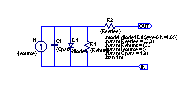
\includegraphics[width=\textwidth]{images/ltspice/singlecell.eps}
    \caption{%
        Schaltung        zur         Simulation        einer        Solarzelle
        gem\"ass        Abbildung       \ref{fig:circuit:solarCell}        von
        Seite     \pageref{fig:circuit:solarCell}. Die     Solarmodule     aus
        den     Abbildungen    \ref{fig:ltspice:module:cellBased:36x2}     und
        \ref{fig:ltspice:module:cellBased:72x1}  basieren auf  Zellen gem\"ass
        diesem Schaltschema.%
    }
    \label{fig:ltspice:solarCell}
\end{figure}

\begin{figure}[h!tb]
    \centering
    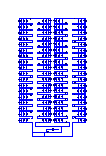
\includegraphics[width=\textwidth]{images/ltspice/module-72cells.eps}
    \caption{%
        Solarmodul     \"ahnlich     zu    Sunset     Solargenerator     AS150
        \cite{ref:solar:as150}, modelliert durch 2  parallele Str\"ange mit je
        36 Zellen gem\"ass Abbildung \ref{fig:ltspice:solarCell} in Serie.%
    }
    \label{fig:ltspice:module:cellBased:36x2}
\end{figure}

\begin{figure}[h!tb]
    \centering
    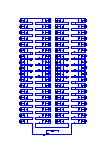
\includegraphics[width=\textwidth]{images/ltspice/module-72cells-series.eps}
    \caption{%
        Solarmodul   \"ahnlich   zu   Sunmodule  Pro-Series   XL   SW320   aus
        \cite{ref:solar:sunmodulePro},  modelliert durch  einen Strang  mit 72
        Zellen gem\"ass Abbildung \ref{fig:ltspice:solarCell} in Serie.%
    }
    \label{fig:ltspice:module:cellBased:72x1}
\end{figure}
\todo{Transistoren aus Schaltbildern entfernen, IN/OUT benennen, Abbildung sollte nur Modul sein}


% ---------------------------------------------------------------------------- %
\clearpage
\section{Vereinfachtes Modell f\"ur ein PV-Modul}
\label{app:models:develop:module:simple}
% ---------------------------------------------------------------------------- %

Zur  Reduktion des  Rechenaufwands im  Vergleich zu  dem im  vorigen Abschnitt
entwickelten Modell soll ein vereinfachtes Modell eines Solarmoduls entwickelt
werden.

Ausgangspunkt   ist   das   Eindiodenmodell    einer   Zelle   aus   Abbildung
\todo{reference}, f\"ur  welches die Parameter  so angepasst werden,  dass das
Verhalten des aus Zellen aufgebauten Modells aus dem vorigen Abschnitt und des
vereinfachten Modells zufriedenstellend \"ubereinstimmen.

Das Vorgehen ist dabei wie folgt: \todo{Eigentliche Werte}

\begin{itemize}
    \item
        Die parasit\"are  Kapazit\"at des  Moduls wird angepasst  gem\"ass dem
        Gesetz zur Serieschaltung von Kapazit\"aten:
        $C_{\mathrm{p, Modul}} = C_{\mathrm{p, Zelle}} \div \text{Anzahl Zellen}$
    \item
        Der Seriewiderstand des Moduls ist die Summe der Seriewiderst\"ande aller
        Zellen
    \item
        Der  Parallele   Widerstand  wird   entsprechend  der   Anzahl  Zellen
        hochgerechnet.
        \todo{kein Einfluss, verifikation}
    \item
        Der Reverse  Saturation Current  des Moduls ist  von der  Fl\"ache des
        Moduls abh\"angig und  wird als Startwert vorerst  gem\"ass der Anzahl
        Module hochgerechnet.
    \item
        Der  Idealit\"atsfaktor ist  ein Indikator  f\"ur den  Spannungsabfall
        \"uber   einer   Diode   bei   einem   bestimmten   Strom   \todo{ref:
        abbildung}. Bei  einer Serieschaltung  von Dioden  sollte entsprechend
        mehr   Spannung    \"uber   dem   gesamten   Strang    abfallen   (bei
        gleichbleibendem  Strom). Der Startwert  f\"ur den  Idealit\"atsfaktor
        des vereinfachten Modells wird  deshalb entsprechend der Anzahl Zellen
        im Modul skaliert.
\end{itemize}

Gem\"ass dieser Methodik werden die Startwerte festgelegt auf:

\begin{itemize}
    \firmlist
    \item
        $C_{\mathrm{p, Modul}} = \SI{167}{\nano\farad}$
    \item
        $R_{\mathrm{S}} = \SI{12}{\milli\ohm}$
    \item
        $R_{\mathrm{Shunt}} = \SI{60}{\kilo\ohm}$
    \item
        $I_{\mathrm{S}} = \SI{288}{\milli\ampere}$
    \item
        $n = 118$
\end{itemize}

Mit diesen  Werten werden verschiedene  Szenarien simuliert und  die Resultate
mit den  Ergebnissen des komplexeren Modells  verglichen. Durch Iteration wird
$I_{\mathrm{S}}$ schlussendlich  auf \SI{2.88}{\micro\ampere}  festgelegt, was
kurioserweise kleiner ist als der Wert einer einzelnen Diode.

Abbildungen
\ref{fig:model:simpel:verif:current:mosfet:freq},
\ref{fig:model:simpel:verif:voltage:mosfet:freq},
\ref{fig:model:simpel:verif:current:RL:freq} und
\ref{fig:model:simpel:verif:current:mosfet:time} stellen die Resultate
verschiedener Simulationen mit und ohne Last f\"ur das vereinfachte Modell und
das zellenbasierte  Modell graphisch dar.   Wie zu erkennen ist,  besteht eine
gute \"Ubereinstimmung.

%Parasit\"are Kapazit\"at: Kapazit\"at einer Zelle / anzahl Zellen \\
%Serie widerstand: widerstand einzelzelle * anzahl zellen \\
%shunt widerstand: widerstand einer zelle / anzahl zellen \\
%IS: IS einzelzelle * anzahl zellen (0.288m) -> anpassen, bis frequenzgang und zeitplot passend \\
%N: N einzelzelle * anzahl zellen \\
%Shockley diode model \\
\todo{Einheiten achsen, auflistung parameter, schaltkreise zu plots, LTspice diagramme}


\begin{figure}
    \begin{tikzpicture}
       \begin{scope}[x={(0mm,0mm)},y={(90mm,0.9\textwidth)}]
           \begin{axis}[%
                   xmode=log,
                   height=45mm,
                   width=0.9\textwidth,
                   at={(0,45mm)},
                   grid=both,
                   xlabel=Frequenz (\si{\hertz}),
                   ylabel=Strom (\si{\deci\bel}),
               ]
                \addplot[color=blue] table {data/simple-model-verification/module-72cells-series--reference--freq-sweep-over-mosfet-no-load--I--magn.dat};
                \addplot[color=magenta] table {data/simple-model-verification/module-simple-72x1--freq-sqeep-over-mosfet-no-load--I--magn.dat};
           \end{axis}
           \begin{axis}[%
                   xmode=log,
                   height=45mm,
                   width=0.9\textwidth,
                   at={(0,0)},
                   grid=both,
                   xlabel=Frequenz (\si{\hertz}),
                   ylabel=Phase (\si{\degree}),
               ]
                \addplot[color=blue] table {data/simple-model-verification/module-72cells-series--reference--freq-sweep-over-mosfet-no-load--I--phase.dat};
                \addplot[color=magenta] table {data/simple-model-verification/module-simple-72x1--freq-sqeep-over-mosfet-no-load--I--phase.dat};
           \end{axis}
       \end{scope}
   \end{tikzpicture}
    \caption{Frequenzgang des Stroms durch den MOSFET bei einer Beschaltung ohne zus\"atzliche Last}
    \label{fig:model:simpel:verif:current:mosfet:freq}
\end{figure}

\begin{figure}
    \begin{tikzpicture}
       \begin{scope}[x={(0mm,0mm)},y={(90mm,0.9\textwidth)}]
           \begin{axis}[%
                   xmode=log,
                   height=45mm,
                   width=0.9\textwidth,
                   at={(0,45mm)},
                   grid=both,
                   xlabel=Frequenz (\si{\hertz}),
                   ylabel=Spannung (\si{\deci\bel}),
               ]
                \addplot[color=blue] table {data/simple-model-verification/module-72cells-series--reference--freq-sweep-over-mosfet-no-load--U--magn.dat};
                \addplot[color=magenta] table {data/simple-model-verification/module-simple-72x1--freq-sweep-over-mosfet-no-load--U--magn.dat};
           \end{axis}
           \begin{axis}[%
                   xmode=log,
                   height=45mm,
                   width=0.9\textwidth,
                   at={(0,0)},
                   grid=both,
                   xlabel=Frequenz (\si{\hertz}),
                   ylabel=Phase (\si{\degree}),
               ]
                \addplot[color=blue] table {data/simple-model-verification/module-72cells-series--reference--freq-sweep-over-mosfet-no-load--U--phase.dat};
                \addplot[color=magenta] table {data/simple-model-verification/module-simple-72x1--freq-sweep-over-mosfet-no-load--U--phase.dat};
           \end{axis}
       \end{scope}
   \end{tikzpicture}
    \caption{Frequenzgang der Spannung \"uber dem MOSFET bei einer Beschaltung ohne zus\"atzliche Last}
    \label{fig:model:simpel:verif:voltage:mosfet:freq}
\end{figure}

\begin{figure}
    \begin{tikzpicture}
       \begin{scope}[x={(0mm,0mm)},y={(90mm,0.9\textwidth)}]
           \begin{axis}[%
                   xmode=log,
                   height=45mm,
                   width=0.9\textwidth,
                   at={(0,45mm)},
                   grid=both,
                   xlabel=Frequenz (\si{\hertz}),
                   ylabel=Spannung (\si{\deci\bel}),
               ]
                \addplot[color=blue] table {data/simple-model-verification/module-72cells-series--reference--freq-sweep-over-Rload--100ohm-100uF--I--magn.dat};
                \addplot[color=magenta] table {data/simple-model-verification/module-simple-72x1--freq-sweep-over-Rload--100ohm-100uF--I--magn.dat};
           \end{axis}
           \begin{axis}[%
                   xmode=log,
                   height=45mm,
                   width=0.9\textwidth,
                   at={(0,0)},
                   grid=both,
                   xlabel=Frequenz (\si{\hertz}),
                   ylabel=Phase (\si{\degree}),
               ]
                \addplot[color=blue] table {data/simple-model-verification/module-72cells-series--reference--freq-sweep-over-Rload--100ohm-100uF--I--phase.dat};
                \addplot[color=magenta] table {data/simple-model-verification/module-simple-72x1--freq-sweep-over-Rload--100ohm-100uF--I--phase.dat};
           \end{axis}
       \end{scope}
   \end{tikzpicture}
   \caption{Frequenzgang des Stroms durch den Lastwiderstand bei einer Last von \SI{100}{\ohm} parallel zu \SI{100}{\micro\farad}}
    \label{fig:model:simpel:verif:current:RL:freq}
   %\label{fig:freqresponse:module:simple}
\end{figure}


\begin{figure}
    \begin{tikzpicture}
       \begin{scope}[x={(0mm,0mm)},y={(60mm,0.9\textwidth)}]
           \begin{axis}[%
                   height=60mm,
                   width=0.9\textwidth,
                   at={(0,0)},
                   grid=both,
                   xlabel=Zeit (\si{\second}),
                   ylabel=Strom (\si{\ampere}),
               ]
                \addplot[color=blue] table {data/simple-model-verification/module-72cells-series--reference--time-domain-over-mosfet-10kHz--I.dat};
                \addplot[color=magenta] table {data/simple-model-verification/module-simple-72x1--time-domain-over-mosfet--10kHz--I.dat};
           \end{axis}
       \end{scope}
   \end{tikzpicture}
    \caption{Zeitlicher Verlauf des Stroms durch den MOSFET bei einer Beschaltung ohne zus\"atzliche Last}
    \label{fig:model:simpel:verif:current:mosfet:time}
\end{figure}


% ---------------------------------------------------------------------------- %
\clearpage
\section{DC-Leitung}
\label{app:models:develop:DCLine}
% ---------------------------------------------------------------------------- %

\todo{Induktivit\"at}
\todo{Kapazit\"at}
